\documentclass [PhD] {uclathes}
\usepackage{graphicx}
\usepackage[table]{xcolor}
\usepackage{epsfig}
\usepackage{cite}
\usepackage{verbatim}
\usepackage{caption}
\usepackage{subcaption}

% \input {mymacros}                         % personal LaTeX macros

%%%%%%%%%%%%%%%%%%%%%%%%%%%%%%%%%%%%%%%%%%%%%%%%%%%%%%%%%%%%%%%%%%%%%%
%
% Usually things live in separate flies.
%
% \input {prelim}                           % preliminary page info

%%%%%%%%%%%%%%%%%%%%%%%%%%%%%%%%%%%%%%%%%%%%%%%%%%%%%%%%%%%%%%%%%%%%%%%%
%                                                                      %
%                          PRELIMINARY PAGES                           %
%                                                                      %
%%%%%%%%%%%%%%%%%%%%%%%%%%%%%%%%%%%%%%%%%%%%%%%%%%%%%%%%%%%%%%%%%%%%%%%%

\title          {Communication Paradigms for Mobile Ad Hoc Networks}
\author         {Justin Scott Collins}
% Note: department is really your area of research.  I.e. leave out 'Department of'.
\department     {Computer Science}
% Note:  degreeyear should be optional, but as of  5-Feb-96
% it seems required or you get a year of ``2''.   -johnh
\degreeyear     {2014}

%%%%%%%%%%%%%%%%%%%%%%%%%%%%%%%%%%%%%%%%%%%%%%%%%%%%%%%%%%%%%%%%%%%%%%%%

\chair          {Rajive Bagrodia}
\member         {Co-chair 3 name}
\member         {Co-chair 2 name}
\member         {Co-chair 1 name}

%%%%%%%%%%%%%%%%%%%%%%%%%%%%%%%%%%%%%%%%%%%%%%%%%%%%%%%%%%%%%%%%%%%%%%%%

\dedication     {\textsl{}}

%%%%%%%%%%%%%%%%%%%%%%%%%%%%%%%%%%%%%%%%%%%%%%%%%%%%%%%%%%%%%%%%%%%%%%%%

\acknowledgments {(Acknowledgments omitted for brevity.)}

%%%%%%%%%%%%%%%%%%%%%%%%%%%%%%%%%%%%%%%%%%%%%%%%%%%%%%%%%%%%%%%%%%%%%%%%

%
% UCLA Policy on Vita
% For security reasons, UCLA policy specifies that your birth year and birth place should not be included in your vita.
%
\vitaitem   {2002--2006}
                {Law School Helpdesk Specialist,
                Seattle University, Seattle, Washington.}
\vitaitem   {2006}
                {B.S.~(Computer Science),
                Seattle University}
\vitaitem   {2007--2010}
                {Graduate Student Researcher, Computer Science Department, UCLA.}
\vitaitem   {2010-2012}
                {Security Engineer, AT\&T Interactive, Glendale, California}
\vitaitem   {2012--present}
                {Security Engineer, Twitter, Inc., San Francisco, California}

%%%%%%%%%%%%%%%%%%%%%%%%%%%%%%%%%%%%%%%%%%%%%%%%%%%%%%%%%%%%%%%%%%%%%%%%

\publication    {J. Collins and D. Joslin. "Improving genetic algorithm performance with intelligent mappings from chromosomes to solutions." In Proc. of the 8th Annual Conference on Genetic and Evolutionary Computation (GECCO '06) (Seattle, Washington, USA, July 08 - 12, 2006).}

\publication    {D. Joslin and J. Collins. "Greedy transformation of evolutionary algorithm search spaces for scheduling problems." IEEE Congress on Evolutionary Computation, 2007 (CEC 2007).}

\publication    {Justin Collins and Rajive Bagrodia. "Programming in Mobile Ad Hoc Networks." In Proceedings of the Fourth International Wireless Internet Conference (WICON 2008).}

\publication    {Justin Collins and Rajive Bagrodia. "A Quantitative Comparison of Communication Paradigms for MANETs." In Proc. of the 7th International ICST Conference on Mobile and Ubiquitous Systems: Computing, Networking and Services (MobiQuitous 2010).}

\publication    {Justin Collins and Rajive Bagrodia. "MELON: A Persistent Message-Based Communication Paradigm for MANETs." In Proc. of the 10th International ICST Conference on Mobile and Ubiquitous Systems: Computing, Networking and Services (MobiQuitous 2013).}

%%%%%%%%%%%%%%%%%%%%%%%%%%%%%%%%%%%%%%%%%%%%%%%%%%%%%%%%%%%%%%%%%%%%%%%%

\abstract {

}
%%%%%%%%%%%%%%%%%%%%%%%%%%%%%%%%%%%%%%%%%%%%%%%%%%%%%%%%%%%%%%%%%%%%%%%%



\begin {document}
\makeintropages

%%%%%%%%%%%%%%%%%%%%%%%%%%%%%%%%%%%%%%%%%%%%%%%%%%%%%%%%%%%%%%%%%%%%%%

\chapter{Introduction}

\section{Motivation}

Mobile ad hoc networks (MANET) comprised of small, mobile, wireless devices present a new and challenging area for the development and deployment of applications. As consumer devices equipped with WiFi capabilities such as smartphones become more widespread, the possibility of impromptu networks also increases. Mobile applications are no longer limited to stand-alone or client-server programs, but can interact and form useful networks directly with each other. Such networks are ideal for situations in which there is no time to set up a fixed access point, or when there is no fixed infrastructure available. Many new applications, particularly in the consumer space, are being applied to MANET, including collaborative software such as shared whiteboards, impromptu networks for communication and entertainment, and peer-to-peer applications for file sharing. While typical examples of MANETs include military units or disaster recovery scenarios, MANETs are also useful inside buildings where cellular reception might be unavailable, where censorship blocks free speech, or even for instant networked gaming between nearby friends.

In mobile ad hoc networks (MANET), high nodal mobility causes frequent topology and route changes, making it difficult to maintain network connections between nodes. Many routes in the network span multiple wireless hops and may experience dramatic and unexpected fluctuations in quality. The combination of mobility and wireless communication creates highly dynamic network topologies in which frequent, possibly permanent disconnections are commonplace, rather than exceptional events. The dynamics of the network and the wireless channel requires changes to the networking stack and alternative solutions at the application level.

While there has been a large amount of work focused on the network stack for MANETs, especially routing, the application layer is not insulated from the challenges faced at the networking layers. Mobile applications face several challenges when compared with programs intended for standard desktops: mobile devices are generally constrained in many ways: the screen size, processor power, memory, and battery power are often limited. Development platforms for mobile devices typically provide basic libraries for application support such as menus and access to data stored on the device. Networking, however, is generally limited to sockets, TCP/IP, and HTTP. In particular, applications are expected to either be stand-alone, like a calculator, or to only be using the network in a client-server manner, such as accessing websites or email servers.

However, most laptop computers are already equipped with WiFi which can operate in ad-hoc mode. Smartphones with WiFi are becoming ubiquitous. In 2013, surveys showed 91\% of adults in the United States had cell phones, and 56\% of those are smartphones\cite{cellphones}. Among teens, 78\% had a cell phone, of which 37\% are a smartphone\cite{teenphones}. Add smartphones to the proliferation of tablets and laptops and the ability for consumers to form mobile ad hoc networks (MANETs) is quickly becoming possible. However, applications designed for these networks remain in short supply.

One way to encourage creation of MANET applications is to simplify communication between devices. Given the challenges of distributed communication in such volatile networks, MANET applications often implement an abstraction layer for network communication. The majority of these abstraction layers are based on traditional distributed computing paradigms which were not designed for unreliable, rapidly-changing wireless networks. We have examined these paradigms and the performance of their implementation for MANETs and found them to be unsuitable for general purpose communication needs of MANET applications. Therefore, we have designed a new communication paradigm specifically to meet the challenges of MANETs, rather than modify an existing paradigm which was not originally intended for the MANET environment.

\section{Contributions}

The first contributions of this dissertation are two comparative studies of communication paradigms used in MANET applications. The first study is a survey of existing libraries and languages used to support MANET applications. Included in the survey is a quantitative comparison using a subset of the surveyed projects to examine how well they perform in a realistic MANET environment. This was the first such quantitative comparison of these projects in identical scenarios.

Once we had surveyed existing projects, it became clear the majority of projects rely on three traditional distributed computing paradigms: publish/subscribe, remote procedure calls, and tuple spaces. In the previous study, we compared performance of projects, but the implementations were in different languages with different levels of completeness and rigor. This made it difficult to conclude anything regarding the underlying communication paradigms. To directly compare the paradigms themselves and determine their suitability as the basis for MANET applications, we implemented canonical versions of the paradigms with as much shared code as possible. In the second contribution of this dissertation, we investigated the impact of wireless and mobility at the application layer for the different paradigms via an emulated network stack, detailed wireless models, and real applications.

After studying the traditional communication paradigms and their adaptations to the MANET context, we designed a new paradigm, MELON, to specifically to meet the challenges of distributed communication in MANETs. MELON provides message persistence, reliable FIFO multicast, read-only messages, simple message streaming, private messages, and efficient bulk operations. To operate well in the distributed and unreliable MANET environment, the design of MELON avoids any global state or locking and performs all operations on-demand. Thus, the third contribution in this dissertation is the design of the MELON communication language.

Our fourth contribution is a prototype implementation of MELON. In order to evaluate the practicality of using MELON in MANET applications, we implemented a prototype of MELON as well as implementing better versions of the three traditional paradigms from above. Again, the four paradigms share as much code as possible in order to eliminate performance differences caused by different implementations. We then compared the performance of MELON with the three traditional paradigms. Besides the quantitative comparison, we also implemented several example applications using MELON to demonstrate its utility in a number of scenarios.

Finally, while empirically evaluating all these paradigms, we created an experiment coordination framework implemented using MELON itself, which is presented as a case study in Section \ref{casestudy:coordinator}. The framework is responsible for managing the network emulator, running the applications under review, collecting output from the applications, and collating the results. It also coordinates the emulator and applications to start and stop at the same time, as well as communicating experiment parameters to the applications. This experiment coordination framework is the final contribution of this dissertation.

\section{Dissertation Organization}

The remainder of this dissertation is laid out as follows:

Chapter \ref{chapter:paradigms} reviews the challenges presented by MANETs and the fundamental communication paradigms which have been applied to MANET applications. In Chapter \ref{chapter:existing} we compare existing projects providing communication libraries for MANETs as well as canonical implementations of the underlying communication paradigms. We present both qualitative and quantitative analysis of the projects and paradigms. Chapter \ref{chapter:model} presents the design of MELON and its communication model, then covers the prototype implementation of MELON in Chapter \ref{chapter:implementation}.

Several case studes are presented in Chapter \ref{chapter:cases} using MELON in applications, including the experiment coordination framework used in our later evaluations. Chapter \ref{chapter:evaluation} includes performance comparisons between MELON and traditional communication paradigms and discusses the suitability of MELON as a basis for MANET applications. Finally, our results and future work are presented in Chapter \ref{chapter:conclusions}. Full MELON application code for a news server/reader and a chat room example may be found in Appendix A.
\chapter{Communication Paradigms for MANETs}

Describe here what is meant by "communication paradigms"

\section{Mobile Ad Hoc Network Characteristics}

Mobile ad hoc networks (MANETs) are composed of mobile nodes which may join or leave the network at any point. These nodes are typically small and battery-powered, such as smartphones, smart watches, PDAs, tablets, netbooks, or laptops. MANETs are not limited to such small nodes, however. They can include unmanned aerial vehicles (UAVs), passenger vehicles, buses, commercial trucks, and any other kind of mobile device. Typically, though, MANETs are expected to be mostly devices with limited battery, processing power, memory, and storage.

Besides being mobile, the other main characteristic of MANETs is their communication via an infrastructureless wireless network. In other words, nodes wirelessly communicate directly with each other or by using other nodes to relay messages. The networks are entirely self-organizing and, in the most general case, rely on no access points, cellular towers, or any other type of fixed wireless receiver.

Mobility and wireless are at the root of all of the challenges MANET applications face. The network topology can change rapidly with nodes joining and leaving at any time without warning, leading to lost information and broken network routes. Wireless communication can be disrupted in many ways, including competing broadcasts, physical obstacles, and nodal mobility.

\section{Requirements}\label{sec:manetrecs}

Based on the characteristics of MANETs, we have identified three key challenges when creating applications to operate in MANETs.

\subsection{Disconnection Handling}

Due to the unreliability of wireless communication and the ability of nodes to physically move, applications in MANETs can experience frequent disconnections. Unlike traditional distributed computing, which typically views disconnections as exceptional events and errors, applications in MANETs must be able to handle disconnections as part of their normal operation.

In a MANET, nodes are highly mobile and disconnections occur frequently, either due to channel condition variation or the mobility of destinations and intermediate nodes. Disconnections may be prolonged, brief, or intermittent and applications must handle all three. Traditional networking treats disconnections as failures, but a programming environment for MANETs needs to handle disconnections as a natural element of the environment.

\subsection{Addressing and Discovery}

The lack of infrastructure in a MANET requires a decentralized method for finding and addressing resources. Traditional approaches such as DNS cannot be maintained in a MANET, so alternative means of discovering and addressing resources must be provided. The spontaneous nature of MANETs also dictates that discovery be dynamic, as the network topology cannot be known ahead of time and may change rapidly.

Unlike a wired network with a fixed infrastructure, MANETs cannot depend on centralized look up services like DNS to find peers. Since devices are constantly joining and leaving the network and it is not possible to maintain IP addresses or URLs to locate resources, applications must be able to locate them dynamically.

\subsection{Flexible Communication}

Basic communication between devices in a wired network is generally accomplished in a one-to-one unicast manner. However, in a MANET, group communication is also common due to the broadcast nature of wireless networking and bandwidth limitations. Collaborative applications, networked games, and streaming media also benefit from group communication.

In order to support generic application development, any communication paradigm needs to support both unicast and multicast communication.

Both unicast and multicast communications are common in MANET applications, which are often group-based or collaborative. Providing flexible communication is crucial to developing applications for MANETs.

\section{Middleware and Languages for MANETs}

Work in this area has mostly focused on adapting existing distributed computing paradigms to the mobile ad hoc environment. Three such paradigms are publish/subscribe, remote procedure calls, and tuplespaces.

It is useful to describe these communication paradigms in terms of temporal and referential (or spatial) coupling~\cite{distbook}. When a paradigm is temporally coupled, it requires the sender and the receiver to both be present when the message is sent. If it is temporally decoupled, a message will be stored and then delivered when the receiver becomes available. Referential coupling indicates whether or not the sender and receiver need to be directly aware of each other. A referentially coupled system explicitly addresses receivers, while a referentially uncoupled system does not need to know with which nodes it is communicating. 

Both temporal and referential uncoupling are preferred in a MANET. If a paradigm is temporally uncoupled, it is more likely to be able to handle disconnections and changing network topologies. Referential uncoupling is useful, because it avoids the need for a centralized naming system and allows remote resources to be addressed using application-level semantics, rather than having to drop down to the network layer.

\subsection{Publish/Subscribe}

Publish/subscribe is a messaging system in which nodes may subscribe to various topics. Nodes publish messages to certain topics, which are then delivered to nodes subscribed to that topic. Typically, there is a system of fixed nodes which serve as \textit{brokers} which manage subscriber lists and delivery of messages. However, the brokering system is completely transparent to the application layer, which is only able to subscribe to topics and publish messages. This maintains the referential decoupling that publish/subscribe systems provide. Published messages may or may not be persistent, depending on the implementation.

Publish/subscribe is completely oriented towards group communication. The only method of communication is publishing a message to a topic. There may be zero or more subscribers to that topic, all of which will receive the message, provided the subscribers are available. One-to-one communication can only be achieved by coordination at the application layer. For example, two nodes may agree to communicate via a topic which they assume no one else will use.

STEAM (Scalable Timed Events and Mobility)\cite{steam} is an example of an event-based middleware which uses publish/subscribe for communication. REDS (REconfigurable Dispatching System) is a framework for building publish/subscribe systems in highly dynamic networks.

\subsection{Remote Procedure Call}

Remote procedure call (RPC) is a form of message passing in which remote procedures or method invocations are syntactically similar or identical to local function calls, but the code is actually executed on a remote machine. When the procedure is called, arguments are copied to the remote machine, which executes the requested method and sends the resulting value back to the local machine. Like publish/subscribe, RPC is temporally coupled, since remote methods must be available at the time of the call. However, RPC is referentially uncoupled, since the application does not know which node it is communicating with, only that it supports a given method.

RPC inherently supports one-to-one two-way communication. Arguments to a method can be considered sending a message, and the return value of the method can be thought of as sending a reply message. RPC can also support group communication by invoking a given method on multiple remote hosts.

Many-to-Many Invocation (M2MI)\cite{m2mi} is an RPC implementation for MANETs which avoids costly ad hoc routing and discovery by broadcasting messages. Messages are addressed by object type, so if a device hosts an object of the addressed type, it will pass the message to that object.

The advantage of M2MI is simplicity. As messages are simply broadcast without expectation of reply, there is no need to worry about return values or blocking while waiting for confirmation. At the language level, there is no difference on the sender's side between a message which is actually received and one which is not received by anyone. Though this provides simplicity, it also means more work for the programmer. As there is no guarantee of message delivery, any functionality beyond simple unidirectional message passing must be implemented on top of M2MI.

AmbientTalk\cite{ambienttalk} is a complete object oriented language inspired in part by M2MI's message passing. AmbientTalk implements a higher level abstraction of resource discovery and disconnection handling which is absent from M2MI, but retains the idea of object handles and remote method invocations. All remote events are handled asynchronously by AmbientTalk through the registration of callbacks. A block of code may be registered to be invoked when discovering a certain resource type. AmbientTalk also adds the ability to receive values from method invocations on remote objects through the use of futures. By default, messages sent to remote objects are buffered until they can be sent. The programmer can also choose to break the connection and recall buffered messages.

\subsection{Tuple Spaces}

Tuple spaces are a form of distributed shared memory. Conceptually, ordered tuples with typed fields are written out to a shared memory space. The tuples can then be read or retrieved by matching them to templates. Applications are associated with one or more tuple spaces, which allows them to access any tuples stored in that space. Three basic operations are defined to manipulate the tuple space: \textit{in()}, \textit{out()}, and \textit{rd()}, which take, write, and read tuples from the shared tuple space. \textit{in()} and \textit{rd()} use tuple templates which are matched against available tuples. There are also non-blocking versions of \textit{in()} and \textit{rd()} called \textit{inp()} and \textit{rdp()} which return immediately even if there are no matching tuples.

Tuple spaces are both temporally and referentially uncoupled. Tuples may be read any time after they have been written to the tuple space, provided they have not been removed in the meantime. Where a tuple may reside is completely unknown to the application; all communication is performed by requesting a tuple matching a particular template. Tuple spaces easily support group communication, since a single tuple may be read by any number of nodes. One-to-one communication can be achieved by agreement on a particular tuple field, although this does not guarantee unintended receivers will not read or even remove the tuple.

LIME (Linda in mobile environment)~\cite{lime} is a well-established implementation of tuple spaces\cite{linda} for mobile environments. Each device or agent has its own tuple space, which can merge with remote tuple spaces when they come into range of each other. Tuples can be read and written from specific locations, but can also be read or written to the ``federated" tuple space which includes the local tuple space and any tuple spaces which are currently merged with it. However, the tuple will reside in a particular tuple space, so when that device or agent moves away, the tuples in that tuple space will move with it and be out of reach. LIME does not currently have an implementation intended for mobile devices smaller than laptops, though there are variations of LIME intended for sensors.

MESH\textit{Mdl}~\cite{meshmdl}  is another tuple space implementation, but varies slightly from the LIME model. In MESH\textit{Mdl}, there is a single tuple space shared between all applications on a device. All communication between applications is performed via  this shared tuple space. Remote tuple spaces are not shared like in LIME, but are accessible for reads and writes only: it is not possible to remove tuples from a remote tuple space. MESH\textit{Mdl} supports mobile agents and recommends using them if actions need to be performed on a remote tuple space. MESH\textit{Mdl} also adds the idea of being able to automatically write, read, or block tuples from other tuple spaces.

Tuples on the Air (TOTA)~\cite{tota}  also implements a tuple space for MANETs, but differs from LIME and MESH\textit{Mdl}. Rather than storing tuples on a particular device, tuples in TOTA are propagated through the network according to rules specified per tuple. As the tuples move through the network, they can acquire context information about the network, such as how many hops they have traveled from the source.

\subsection{Mobile Agents}

Using mobile agents in MANETs allows programs to move code to data, rather than communicating the data to the running program. Code migrates to where data or resources are located, executes at that location, and then returns to its original location to report the results. This allows mobile devices, which usually have little processing power, to offload computationally intensive work to machines with more processing and power resources.

SpatialViews\cite{sv} is a language extension to Java ME which allows programs to iterate over groups of devices. The code inside the loop is executed on the initial device and then migrates to the next, eventually making its way back to the initial node. This allows for complex operations to be written easily, as the language has built-in support for such things actions as reduction operations. The iteration itself is generally done according to some physical layout, although it is possible to iterate over all objects or to use logical locations instead.

\chapter{Analysis of Existing Paradigms}

\section{Project-Based Comparison}\label{sec:proj_eval}

The current projects for developing software in MANETs fall into three broad categories: runtimes, languages, and middleware, which offer increasing levels of abstraction for the developer. They can also be combined: a middleware solution can be written in a language which uses one of the basic runtimes for mobile devices. In many cases projects also provide additional resources for software development such as debuggers and emulators for testing code. Table\ref{table:projs} summarizes the representative projects discussed in this section with respect to the requirements in Section \ref{sec:manetrecs}. Broader overviews focusing only on middleware for MANETs can be found in~\cite{middlewaresurvey} and \cite{newmiddlewaresurvey}.

\begin{table*}
\centering
\caption{Projects Summary}
\begin{tabular}{|c|p{2cm}|p{3cm}|p{4cm}|p{3.5cm}|} \hline
\textbf{Project} & \textbf{Category} & \textbf{Disconnection Handling} & \textbf{Addressing and Discovery} & \textbf{Communication} \\ \hline
LIME & Middleware & Tuple removal & Merged tuple spaces & Tuple space \\ \hline
MESHMdl & Middleware & Tuple removal & Tuple exchange & Tuple space \\ \hline
TOTA & Middleware & Connectionless & Tuple propagation & Tuple space \\ \hline
STEAM & Middleware  & Connectionless & Event content & Publish/subscribe \\ \hline
SyD & Middleware &  Object proxies &  Object type & Message passing \\ \hline
M2MI & Language & Connectionless &  Object type & Message passing \\ \hline
AmbientTalk & Language &  Flexible references &  Object type & Message passing \\ \hline
\begin{comment}YCab & Middleware &  State recovery &  Sessions, handles & Message passing \\ \hline\end{comment}
SpatialViews & Language & Connectionless & Object type & Code migration \\ \hline
.NET CF & Runtime &  None & URL & Sockets \\ \hline
Java ME & Runtime & None & URL & Sockets \\ \hline
\end{tabular}
\label{table:projs}
\end{table*}

\subsection{Project Overview}

\subsubsection{Runtimes}

Runtimes in this context are virtual machines for languages which are specifically intended for use on small, resource-constrained mobile devices. Runtimes are useful because they provide good portability for applications and thereby simplify some of the application development process.

Two common runtimes for mobile devices are Java ME~\cite{javame} and the .NET Compact Framework~\cite{dotnetcf}. A third runtime, BREW~\cite{brew}, is a proprietary product from Qualcomm. These runtimes focus on using few resources and providing libraries for application development, especially user interfaces. They do not provide much networking support beyond basic sockets and HTTP support. While it is possible to use these runtimes as foundations for better abstractions, they provide little on their own to support MANET applications and will not be considered in the following comparisons.

\subsubsection{Languages}

A language in this dissertation refers to any language, language extension, or library which provides new language constructs for programming in a MANET. Languages often include their own runtime or are built on top of existing runtimes. Libraries and language extensions are likely to be easier for developers to use if they are already familiar with the base language.

M2MI~\cite{m2mi}, AmbientTalk~\cite{ambienttalk}, and SpatialViews~\cite{nisv} are three language-based projects intended for MANETs. Many-to-Many Invocation (M2MI) avoids costly ad hoc routing and discovery by broadcasting messages. Messages are addressed by object type, so if a device hosts an object of the addressed type, it will pass the message to that object.

The advantage of M2MI is simplicity. As messages are simply broadcast without expectation of reply, there is no need to worry about return values or blocking while waiting for confirmation. At the language level, there is no difference on the sender's side between a message which is actually received and one which is not received by anyone. Though this provides simplicity, it also means more work for the programmer. As there is no guarantee of message delivery, any functionality beyond simple unidirectional message passing must be implemented on top of M2MI.

AmbientTalk is a complete object oriented language inspired in part by M2MI's message passing. AmbientTalk implements a higher level abstraction of resource discovery and disconnection handling which is absent from M2MI, but retains the idea of object handles and remote method invocations. All remote events are handled asynchronously by AmbientTalk through the registration of callbacks. A block of code may be registered to be invoked when discovering a certain resource type. AmbientTalk also adds the ability to receive values from method invocations on remote objects through the use of futures. By default, messages sent to remote objects are buffered until they can be sent. The programmer can also choose to break the connection and recall buffered messages.

SpatialViews takes a completely different approach than M2MI and AmbientTalk. SpatialViews is a language extension to Java ME which allows programs to iterate over groups of devices. The code inside the loop is executed on the initial device and then migrates to the next, eventually making its way back to the initial node. This allows for complex operations to be written easily, as the language has built-in support for such things actions as reduction operations. The iteration itself is generally done according to some physical layout, although it is possible to iterate over all objects or to use logical locations instead.

\subsubsection{Middleware}

Middleware is software which manages interaction and communication between applications, as well as providing various services which may be used by applications. Middleware may also include supporting libraries which can be used by applications.

LIME (Linda in mobile environment)~\cite{lime} is a well-established implementation of tuple spaces\cite{linda} for mobile environments. Each device or agent has its own tuple space, which can merge with remote tuple spaces when they come into range of each other. Tuples can be read and written from specific locations, but can also be read or written to the ``federated" tuple space which includes the local tuple space and any tuple spaces which are currently merged with it. However, the tuple will reside in a particular tuple space, so when that device or agent moves away, the tuples in that tuple space will move with it and be out of reach. LIME does not currently have an implementation intended for mobile devices smaller than laptops, though there are variations of LIME intended for sensors.

MESH\textit{Mdl}~\cite{meshmdl} is another tuple space implementation, but varies slightly from the LIME model. In MeshMdl, there is a single tuple space shared between all applications on a device. All communication between applications is done through this shared tuple space. Remote tuple spaces are not shared like in LIME, but are accessible for reads and writes only: it is not possible to remove tuples from a remote tuple space. MESH\textit{Mdl} supports mobile agents and recommends using them if actions need to be performed on a remote tuple space. MESH\textit{Mdl} also adds the idea of being able to automatically write, read, or block tuples from other tuple spaces.

Tuples on the Air (TOTA)~\cite{tota} also implements a tuple space for MANETs, but differs from LIME and MESH\textit{Mdl}. Rather than storing tuples on a particular device, tuples in TOTA are propagated through the network according to rules specified per tuple. As the tuples move through the network, they can acquire context information about the network, such as how many hops they have traveled from the source.

Haggle \cite{haggle} is a middleware for mobile networks which allows tagged data to persist in a publicly searchable storage space. The Haggle middleware focuses heavily on abstracting the network layers by implementing its own routing and naming schemes, which allows a single name to map to several addresses such as MAC addresses, phone numbers, or email. Haggle proposes folding in many routing protocols, MAC protocols, and application protocols into the middleware and dynamically selecting and combining them.

SyD (System on Mobile Devices)~\cite{syd} is a complete middleware solution for MANETs. The middleware centers around the idea of object registries which allows service registration and lookup. Methods can then be invoked on these remote objects. Disconnection is handled by allowing objects to also provide proxy objects. If an object is unavailable, the method invocation will be handled by the proxy object, which can then perform an action specific to that service. For example, the proxy may buffer the request and send it later, or send back a cached or default response.

STEAM (Scalable Timed Events and Mobility)~\cite{steam} is an event-driven middleware which uses a publish/subscribe\cite{psfaces} mechanism for propagating events. STEAM uses the concept of proximity groups for communication, limiting events to the local geographic area. Events are propagated by subscribers only when the subject and proximity match. Events are further filtered on the subscriber side by content, which determines if an event is delivered to the local application.

\subsection{Suitability for MANETs}

\subsubsection{Disconnection Handling}

The main challenge in MANETs is handling disconnections, which may be intermittent, prolonged, or permanent. For example, at a busy conference there may be many mobile devices in contact with each other, but distance and physical obstacles may cause intermittent disconnections. Routes may also break and reform due to mobility or channel variations, possibly causing prolonged disconnections, but connections are eventually regained. When the attendees all leave, it becomes unlikely their devices will ever be in contact with each other again, making the disconnection permanent. A programming environment for MANETs must be able to handle all three kinds of disconnections.

One solution, used in LIME, MESH\textit{Mdl}, and TOTA, is to use tuple spaces for communication. Tuple spaces exhibit both spatial and temporal decoupling, meaning that messages being sent do not need to be addressed to a particular recipient nor does the recipient need to be present when the message is sent. Tuple spaces generally operate by reading, writing, and taking tuples to and from a shared location. Rather than sending a message directly to a recipient, a tuple is written to the tuple space and can be read or taken from the tuple space by other clients. This allows the tuple space to withstand disconnections.

For example, a tuple may be written out to the tuple space and then retrieved by a different client an arbitrary amount of time later. The client which retrieves the tuple may not even be in existence when the tuple was written. However, there is still a problem if the writer of the tuple disconnects before the tuple is read by a receiver. For LIME and MESH\textit{Mdl}, where the tuple space is associated with a particular devices, the tuple space is only available when the sender and the receiver are able to communicate directly with each other. In TOTA, tuples are disseminated throughout the network and can survive even if the original sender disconnects.

A different approach, used by M2MI and STEAM, is to forgo connections completely. Messages in M2MI are sent with no expectation of reply. In the general case, messages are sent to a particular object type, to be processed by any device hosting an object of that type. Messages are broadcast with no buffering whether or not there is a receiver available. This provides even more decoupling than tuple spaces, but tuple spaces have the advantage of having some feedback about a tuple's status. The sender can check if a tuple has been removed from the tuple space or not. If it has, the sender can have some assurance the tuple was received by someone, otherwise it will be available until removed by the original sender or another client.

STEAM avoids connections by filtering events on the subscriber's side. This eliminates the need for publishers to keep track of subscribers and completely decouples the two. However, publish/subscribe in a MANET environment does not provide any message reliability. Any message reliability or disconnection feedback would need to be implemented on top of the publish/subscribe framework.

Code migration, the approach used by SpatialViews, does not maintain connections, but can be affected by disconnections if the device currently executing the mobile code fails or leaves the network before completion.  Most of the devices in the network will not be involved in executing code at any particular moment, in which case their failure or disconnection from the network would not have an effect. When it does have an effect, however, it may cause the entire iteration to fail. This can be mitigated by using a form of parallel iteration over the devices. Since the iteration order in SpatialViews is nondeterministic, it does not provide message reliability.

A third approach, implemented in AmbientTalk, relies on event handling and futures. Event handlers can be registered for various events, such as discovery of a service or disconnection of a remote object. Figure~\ref{fig:atpd} illustrates the use of two of these callbacks to discover a printer service. Once a printer is discovered, a document is sent to be printed and a status message is returned.  If a remote object is discovered and later moves out of range, AmbientTalk can call the disconnection code. By default, messages sent to a disconnected remote object will be buffered until it is possible to send them. This provides a solution for intermittent and even prolonged disconnections. If a remote object is disconnected for too long, the programmer can recall all buffered messages and close the connection.

\begin{lstlisting}[caption={Printer Discovery in AmbientTalk}, label={fig:atpd}]
 def print(doc) {
  when: Printer discovered: { |printer|
    when: (printer<-print(doc)) becomes: {|res|
      system.println("Status: " + res);
    };
  };
 };
\end{lstlisting}

AmbientTalk also offers AmbientReferences\cite{ambientrefs}, which are related to the M2MI model of object handles.  AmbientReferences have a specified flexibility which determines how disconnections are handled. Sturdy is the default model of using buffered messages which will be delivered upon reconnection. Elastic references wait a specified amount of time before severing the connection and rebinding to another object of the same type. Fragile references will break immediately upon disconnection and rebind to another object as quickly as possible.

The approach used by SyD is to offer the ability for the application designer to specify how to handle disconnections. In SyD, it is possible to provide proxy objects which will be called when the actual remote object is unavailable. These objects can then handle the invocation in an object-specific manner, such as buffering or returning a default value. \begin{comment}YCab provides an interface for storing application-specific data and restoring the state of the application upon reconnection to a given session.\end{comment}

\subsubsection{Addressing and Discovery}

Unlike a wired network with a fixed infrastructure, MANETs cannot depend on centralized look up services like DNS to find peers. Since devices are constantly joining and leaving the network and it is not possible to maintain IP addresses or URLs to locate resources, applications must be able to locate them dynamically.

The tuple space implementations of LIME, MESH\textit{Mdl}, and TOTA automatically discover neighboring tuple spaces. LIME will merge tuple spaces with the same name, while MESH\textit{Mdl} does not merge tuple spaces, but uses special tuples to provide a method of addressing a remote tuple space. Tuple spaces can be used for service discovery by writing out tuples which describe available services, or by writing out tuples intended for a specific service, which will read the tuples when it is available.

Addressing is not necessary in general in tuple spaces, as it can be assumed a given service and a client will have pre-agreed upon tuple template to use for communication. For example, a ubiquitous application used by a museum might have ``information points'' with information specific to a location. The information point does not need to even be aware of clients, nor do clients need to know any identifying information about the information point, as they will simply read available tuples from the information point's tuple space.

Object types for discovery and addressing is used by M2MI, AmbientTalk, and SpatialViews. This is based on the assumption that objects with the same name will implement the same services. M2MI and AmbientTalk use this with object handles which refer to a specific object type. When methods are invoked on a given handle, the remote object will correspond to the type of the object handle. M2MI, however, does not provide a method for discovery beyond manually sending out messages periodically and waiting for replies. AmbientTalk offers event handlers to be automatically called when objects of a specific type are discovered. These can be called exactly once or each time one is discovered.

SpatialViews uses object types along with spacial properties to define a ``view" of the network. Once a view is created containing a given object type, SpatialViews provides a method of iterating over the available nodes within that view. The code within the iterator is executed locally on the remote devices. After the code is run, the device locates another nearby node hosting an object of the correct type and the code migrates there. Within the iteration, the code can synchronously invoke methods on the local service through an object handle. In Figure~\ref{fig:svsm}, a simple SpatialView is created to broadcast a message in a chat application. The code within the \texttt{visiteach} block (line 4) is executed locally. Therefore, unlike the AmbientTalk printer example, \texttt{c.receive(...)} is a local method call, not a remote call.

\begin{lstlisting}[caption={Simple Messaging in SpatialViews}, label={fig:svsm}]
 spatialview v = ChatService;

 visiteach c : v {
   c.receive(sender, message);
 }
\end{lstlisting}

SyD also uses objects to invoke remote services, but it requires that these objects register themselves with neighboring devices, as well as locally. \begin{comment}YCab is interesting in that it allows applications to detect nearby sessions, then suggest a handle for themselves. If the handle is unique in the session, the client is allowed to join, otherwise the client is rejected. \end{comment}

The publish/subscribe model used by STEAM relies on subscribers knowing ahead of time what subscriptions are interesting to them. The publishers do not need to explicitly know who is subscribed, as messages are simply broadcast. However, it is possible to periodically send out messages describing available subscriptions.

\subsubsection{Flexible Communication}

Basic communication between devices in a network is generally accomplished in a one-to-one unicast manner. However, in a MANET, group communication is also common, due to the broadcast nature of wireless networking and the limitations of bandwidth. Collaborative applications, networked games, and streaming media also benefit from group communication. Having both one-to-one and group communication available in the programming environment is necessary, though it may be possible to implement one with the other.

Tuple spaces lend themselves naturally to group communication. Tuples are written to shared storage space, which is globally accessible. Since tuples can be read without being removed from the tuple space, tuples are inherently one-to-many. One-to-one communication is not as directly supported by tuple space. However, tuples can be sent to a specific recipient by setting one of the fields in the tuple to an agreed-upon address. The specified recipient can look for tuples addressed to itself and take them from the tuple space.LIME, MESH\textit{Mdl}, and TOTA support this type of communication. 

M2MI and AmbientTalk support object references which can refer to all objects of a type, a selected subset of those objects, or a particular object. These handles directly correspond to broadcast, multicast, and unicast. Since AmbientTalk expects return values from messages, it is possible to receive multiple replies when sending a multicast or broadcast message, resulting in event handlers running multiple times or the return value being set more than once.

Communication in SpatialViews is done through code and variable migration. This makes it very simple to perform complex group operations such as reductions over several devices, but it makes one-to-one communication difficult. Figure~\ref{fig:svpd} shows how it is necessary to set a variable to ensure a document is only printed by a single printer. There is also no method to provide reliable message delivery, other than iterating until a prearranged flag is set.

\begin{lstlisting}[caption={Printer Discovery in SpatialViews}, label={fig:svpd}]
 Container result = new Container();
 spatialview v = Printer;
 visiteach p : v {
    if(result.isEmpty()) {
       String result = p.print(document);
	    if(result == "success")
	       result.addElement(p.getName());
    }
 }
\end{lstlisting}

Similarly, publish/subscribe naturally supports group communication, but attempting to send a message to a particular recipient is not directly supported by the middleware. Publish/subscribe is intended to be used in situations with a single sender and multiple receivers and does not adapt well to sending a message to a single receiver. To do so would require the sender and receiver using a predefined addressing, similar to setting an agreed-upon tuple value in tuple spaces. Successful message delivery in the publish/subscribe is less likely than in a tuple space, since messages are not persistent in the way that tuples are.

\begin{lstlisting}[caption={LIME: Print Job Reaction}, label={fig:lpj}]
 LimeTupleSpace lts = 
   new LimeTupleSpace();
 lts.setShared(true);
 ITuple printjob = 
   new Tuple().addFormal(PrintJob.class);
 UbiquitousReaction ur = 
   new UbiquitousReaction(printjob, 
     this, Reaction.ONCEPERTUPLE);
 lts.addWeakReaction(new Reaction[] {ur});
\end{lstlisting}

\subsection{Applications}

To better understand the effect of using different programming approaches when developing applications, two separate applications were written using AmbientTalk, LIME, and SpatialViews. These projects were selected because they represent very different approaches and had publicly available implementations. For each application, we discuss issues with disconnections, discovery, and communication.

\subsubsection{Printer Discovery}

The printer discovery application illustrates how the different projects can be used to approach the problem of resource discovery in a changing network. The client needs to locate a device offering a printer service. Next it sends the print job to a printer it has found, then waits for a reply. The printer processes the job and sends back a success or failure message.

Disconnection can occur at different points in this process. The printer may go out of range after the client has discovered it, but before the job is sent, or it may go out of range after the job is sent, but before the result is returned. In AmbientTalk, the default way of handling both cases is to wait until the printer can be contacted again and then resume the connection. The print job or result message will be buffered until the connection can be made again and then the message will be delivered. This works well in the case where there is only transient disconnection, but if a client has permanently left the area of the printer the application may wait forever unless the programmer explicitly uses a timeout.

In SpatialViews, the only way to communicate between nodes is to visit them in the course of an iteration over all nodes which offer a given service. With the SpatialViews implementation of printer discovery, disconnection after discovery and before sending back the success message are essentially the same. The iteration will never complete and the originating node will eventually timeout.

One of the strengths of tuple spaces is temporal decoupling. The sender and receiver do not both need to be present at the same time for a message to be sent. The LIME version of printer discovery does not face the disconnection issues above, partially because a print job remains in the tuple space until a result tuple is received. A printer which reads the print job and then goes out of range does not affect the operation. If the client is not in range when the result tuple is sent, but reconnects later, the result tuple will still be available for it to read. Even if the client permanently leaves an area, a different printer can pick up the print job instead. The downside of this approach is that multiple printers may process the same job, wasting resources.


In this example, addressing and discovery are needed to find a printer service and also to send the result message. AmbientTalk and SpatialViews handle addressing with interface types. The printer offers a service with a typed interface and the client is able to find nearby services of a given type. Discovery is also built into both AmbientTalk and SpatialViews. In AmbientTalk, a callback function is set up to be called when the printer service is discovered, as shown previously in Figure~\ref{fig:atpd}. SpatialViews uses the idea of an iterator which loops over objects of a certain type nearby. In this respect, AmbientTalk is more reactive, while SpatialViews is proactive. The disadvantage to the SpatialViews approach is the service must be available at the time of the iteration, otherwise it will complete without a result. It will then be up to the programmer to retry the iteration until it is successful.

Discovery in LIME merely requires the registration of reactions to tuple templates. Addressing the printer is not necessary, but the result message contains a print job identifier so the client knows which job it represents.

Printer discovery does not really involve group communication, but there is one-to-one communication in the sending of the print job and the result message. In AmbientTalk, an object handle to the remote printer service is created when the the printer is found. The print job is then sent by invoking a method on the handle and waiting for a return value. On the printer side, it only needs to return a value, it does not require any knowledge of the client.

For SpatialViews, care must be taken to make sure the print job only goes to a single printer. Since the only method of communication is to visit every printer available, it is necessary to set a flag in a shared variable indicating the print job was already successfully printed and subsequent printers do not need to address it, as seen in Figure~\ref{fig:svpd}. Again, the printer does not need to know anything about the client.

In LIME, all communication is also inherently group communication, so the result tuple needs to be explicitly addressed to the client using a some sort of identification. The client will be waiting for a tuple with that specific ID.

\subsubsection{Chat}

The second example is a chat application. Clients can send out public or private messages. Public messages are delivered to all other chat clients nearby, while private messages are directed to a specific recipient. As in most chat applications, there is no history and clients do not expect to receive messages sent earlier or when disconnected. Disconnection can occur at any time while clients are exchanging messages.

Disconnection has less effect in this application than with printer discovery, as the clients do not depend on the delivery of messages to continue operating. However, the AmbientTalk implementation does buffer both public and private messages and delivers them when the client reconnects, as this is built into the language. LIME also handles disconnection well in this case, since there is no need to guarantee message delivery. 

SpatialViews suffers from the same issue in the printer discovery example: if the code migrates to a section of the network which then becomes disconnected from the rest of the network, or the current node goes down, the iteration just stops. Since each message is a separate iteration, it will not affect the overall operation of the application.

Addressing is handled similarly to the printer discovery example, except the user needs to know the names of other users when sending private messages. The AmbientTalk version notifies the user when other clients come into range and adds their name and object handle to a list. Figure~\ref{fig:svchat} shows the implementation of the methods for sending out messages. Public messages are sent out to an AmbientReference, defined in line 1, which only needs to know the interface name and implicitly tracks individual clients.

\begin{lstlisting}[caption={Chat in SpatialViews}, label={fig:svchat}]
def all := ambient: Chatter 
    withCardinality: omni 
    withElasticity: fragile;

def sendAll(message) {
  all<-send(message, name);
};

def send(buddy, message) {
  def b := buddy_list.get(buddy);
  b<-send_private(message, name);
};
\end{lstlisting}

SpatialViews, like in the printer discovery application, iterates over all nodes with the chat interface, delivering the message to each as it visits. This is shown in Figure~\ref{fig:svchat}. For private messages, it still must iterate in the same manner, but the recipient is encoded in the message. Unfortunately, this means private messages still require visiting every node, possibly without even reaching the recipient in the case of disconnection. Likewise, LIME must rely on encoding the recipient in the message tuple and assuming no one but the intended client will read the message.

Group communication is natural for public messages and one-to-one communication for private messages. All three projects handle group communication well. AmbientTalk has omni-handles which refer to all interfaces of a given type and will broadcast the message to all nearby clients. The only communication in SpatialViews and LIME are essentially group communication, so for one-to-one communication, SpatialViews and LIME require the programmer to implement an addressing scheme on top of the group communication. The client side of the application needs to pick out private messages intended for it and ignore the rest.

\subsection{Experimental Results}

This section compares the performance of AmbientTalk, LIME, and SpatialViews in a regular wired LAN and in a MANET context using EXata.

The wired LAN environment provides a nearly ideal network in which the cost of communication is very low, there is little contention for the communication channel, all nodes are connected directly to each other, and collisions are minimal. By minimizing these factors, it is possible to focus the experiment results on the overhead of the programming environments. In these experiments, all nodes were directed connected to a 100Mb/s switch, providing essentially an independent, one hop channel for each pair of nodes

The results using EXata more accurately reflect the MANET environment. For these experiments, all communication was performed through EXata, which emulated an 802.11b ad hoc wireless network with an available bandwidth of 11Mb/s.

\begin{figure}
\centering
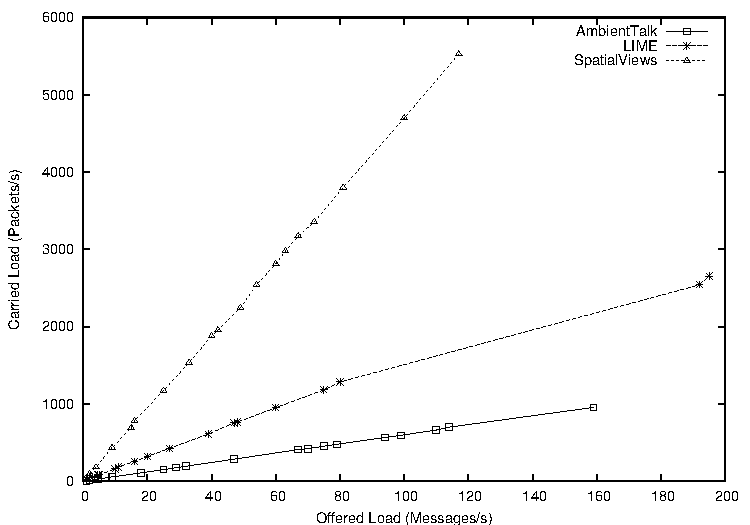
\includegraphics{figures/overhead-wired.pdf}
\caption{Communication Overhead with Wired Links}
\label{fig:overhead-wired}
\end{figure}

\begin{figure}
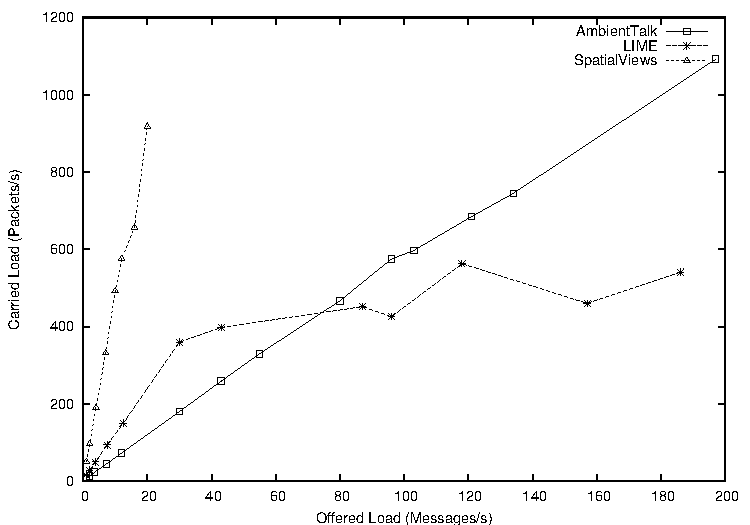
\includegraphics{figures/overhead-qualnet.pdf}
\caption{Communication Overhead with Simulated Wireless Links}
\label{fig:overhead-qualnet}
\end{figure}

\subsubsection{Communication Overhead}

AmbientTalk, LIME, and SpatialViews use very different messaging systems. This experiment demonstrates the overhead for each using a client-server setup as the simplest base case. Messages are sent out from the sever to the client at an increasing rate. The number of IP packets generated by doing so include control and discovery packets. Each node is within wireless range of the others so all communication is performed over single hop routes. Figure~\ref{fig:overhead-qualnet} and Figure~\ref{fig:overhead-wired} show the results from wired LAN and QualNet, respectively.

AmbientTalk has the lowest overhead, as it is simply performing a method call on a remote object and there is no return value. LIME requires some communication to alert merged tuple spaces of the messages' presence and then more communication to actually transfer the tuple. SpatialViews shows the highest amount of overhead, which is expected since it is migrating code and data to communicate a simple message. 

Although the results were similar in the wired LAN and EXata, the performance of SpatialViews was considerably slower, peaking at 20 msgs/s, while in the wired LAN it was possible to reach 117 msgs/s. This is due to contention for the wireless channel. It is also worth considering that LIME and AmbientTalk use asynchronous messages while SpatialViews uses a blocking synchronous message send. This allows LIME and AmbientTalk to take advantage of system level buffers, while SpatialViews cannot.

\begin{figure}
\centering
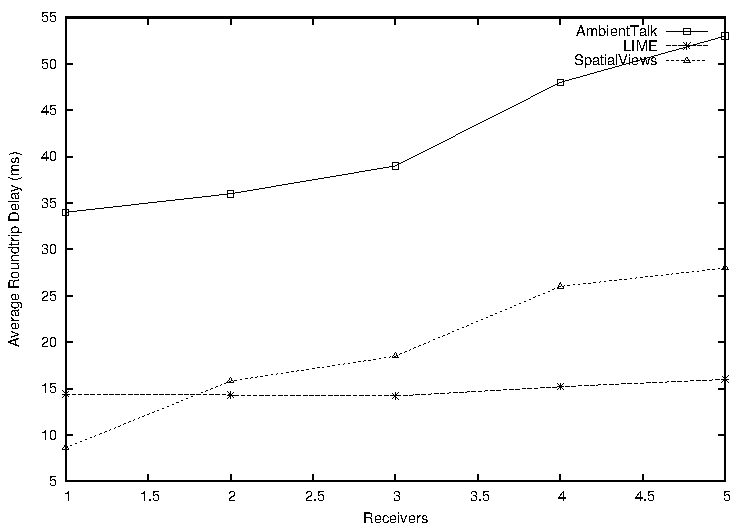
\includegraphics{figures/multicast-wired.pdf}
\caption{Group Communication with Wired Links}
\label{fig:multicast-wired}
\end{figure}

\begin{figure}
\centering
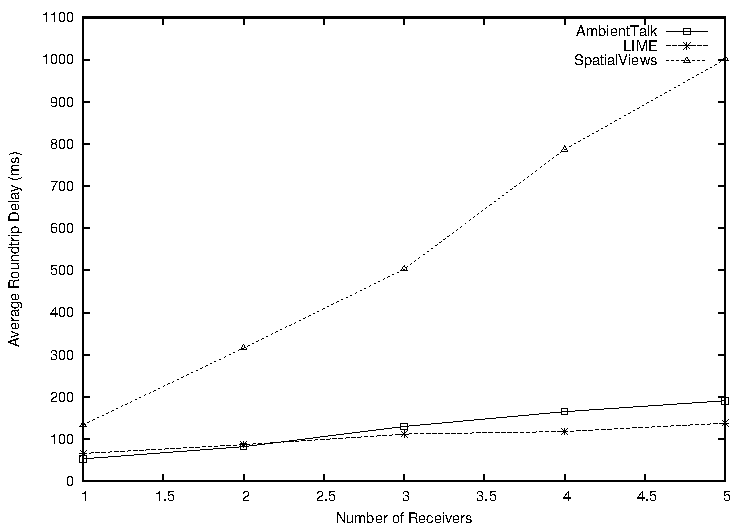
\includegraphics{figures/multicast-qualnet.pdf}
\caption{Group Communication with Simulated Wireless Links}
\label{fig:multicast-qualnet}
\end{figure}

\subsubsection{Group Communication}

In this experiment we consider the common situation where one node needs to request information from the rest of the network and then collect the results, with increasing numbers of receivers. The application sends out a message then measures the time elapsed for responses.  For SpatialViews, this involves visiting each node and that node then visiting the sending node. The AmbientTalk version uses an omnihandle, as in the chat application, to broadcast the handle of the sender and then the receivers use the handle to send a return message. For LIME, each message is sent as a tuple, to which the receivers send a response tuple. Again, the network is set up so that no node is farther than one hop from any other node. Figures~\ref{fig:multicast-qualnet} and ~\ref{fig:multicast-wired} show the results.

In the wired LAN, LIME shows the least variation as the number of receivers increases. This is because the sender writes out a single tuple and each receiver can respond independently and in parallel. SpatialViews slows down considerably as the number of receivers increases, since SpatialViews visits each receiver in turn and waits on a response before continuing. The delay for AmbientTalk is the highest but does not increase quite as quickly as SpatialViews. Although AmbientTalk uses a single send at the application level, messages to individual receivers are sent serially, causing the delay for the last receiver to be higher than the first. 

When run using EXata, the effect of using the wireless channel is seen again. The delay with AmbientTalk and LIME increases, but not as dramatically as SpatialViews, which reaches a delay of about 1 second with 5 receivers, while a single receiver averages 134 ms. As in the previous experiment, the traffic generated by SpatialViews quickly creates conflicts in the wireless channel, causing retransmission and delay at the MAC layer.

\subsubsection{Mobility and Disconnection}

\begin{figure}
\centering
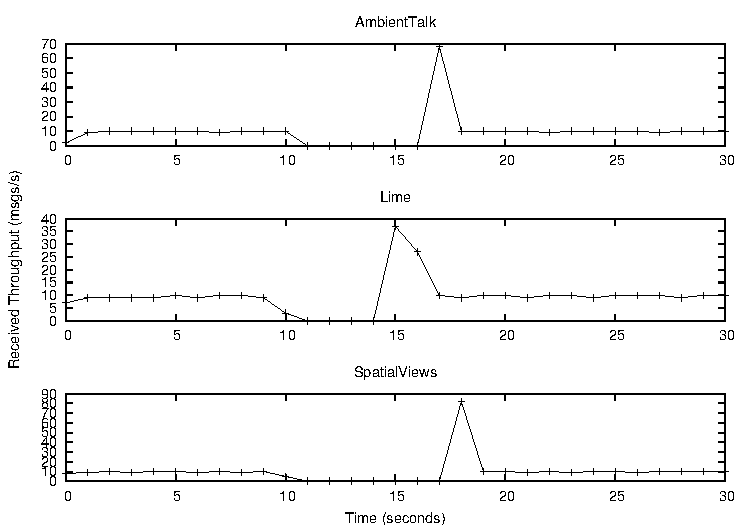
\includegraphics{figures/disconnection.pdf}
\caption{Disconnection Recovery}
\label{fig:disconnection}
\end{figure}

\begin{figure}
\centering
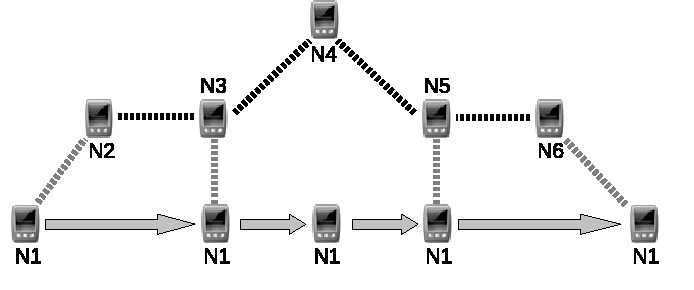
\includegraphics{figures/network.pdf}
\caption{Simulated Mobility Scenario}
\label{fig:network}
\end{figure}

\begin{figure}
\centering
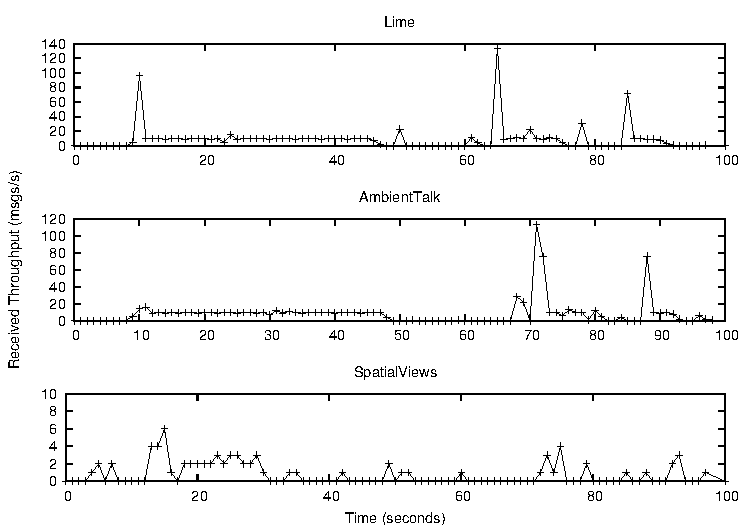
\includegraphics{figures/mobility-results.pdf}
\caption{Client-Server Throughput with Mobility}
\label{fig:mobility-results}
\end{figure}

In order to isolate and examine disconnection recovery, a simpler experiment in a wired LAN was performed, still using the same client-server application. In this case, a 5 second disconnection was caused by turning the network interface off and then turning it back on. Each project reacted similarly, as shown in Figure~\ref{fig:disconnection} though LIME showed the fastest recovery time. Interestingly, SpatialViews exhibited delivery of buffered messages. As SpatialViews does not buffer messages itself, this buffering was the result of the operating system attempting to locate the remote node.

Using EXata, it was possible to evaluate the projects in a mobile environment which provided disconnections, routing changes, and multi-hop communication. For this experiment, the network layout and mobility pattern shown in Figure~\ref{fig:network} was used. Node 1 user the same client-server application as in the first experiment and is attempting to send messages to Node 4. The distance between the two nodes forces a multi-hop route through the intermediate nodes. Node 1 moves from left to right at a constant rate during a time period of 100 seconds. This experiment again measures message delivery rate. Results are shown in Figure~\ref{fig:mobility-results}. 

The large spikes for the AmbientTalk and LIME results indicate the delivery of buffered messages. For AmbientTalk, the sender did not begin until the receiver was discovered, while LIME began sending messages immediately. The flat part of the graphs indicates when Node 1 was in between Node 3 and Node 5 and was outside the range of both. SpatialViews did not perform well in this experiment because it lacks the sophisticated disconnection handling and message buffering of the other two experiments. Also, the code migration was difficult, more time consuming, and more susceptible to disconnections. As in the previous experiments, this demonstrates the difference between experiments using a wired LAN compared to a simulated wireless network. 

\section{Paradigm-Based Comparison}\label{sec:para_eval}

\subsection{Suitability for MANETs}

\subsubsection{Disconnection Handling}

In the unreliable MANET environment, disconnections frequently occur during the exchange of messages. Since disconnections can be prolonged, the networking layers will assume the connection is entirely lost and cease retrying. By having a message persist in some way, a paradigm can overcome these disconnections and deliver the message at a later time.

Publish/subscribe allows message publication without any consideration for the state of the subscribers. Publish/subscribe itself does not specify how ``missed'' publications should be handled. A publish/subscribe system can utilize ``brokers'' which manage subscriptions and facilitate delivery of publications. Brokers can then serve as message buffers and provide more reliable message delivery in the face of disconnections. In distributed publish/subscribe systems, however, the brokers must be self-organizing, and in MANET this is complicated by how quickly the network can change. It is common for distributed publish/subscribe systems not to provide message persistence. If a subscriber is not available at the time of publication, the message will not be received.

Since RPC requires a connection for communication, disconnections typically cause RPC to block a process entirely until a remote node hosting an appropriate method is available. Messages themselves only exist briefly during the RPC transaction. Messages cannot be sent if a connection cannot be made to a remote host.

In tuple spaces and MELON, message persistence is inherent in the paradigms. In both paradigms, exchange of messages is achieved by storing the messages in a shared storage space. Any amount of time may elapse between the storage of a message and its retrieval. This allows reliable communication even in the face of prolonged disconnections and is the reason we have chosen it for MELON.

\subsubsection{Addressing and Discovery}

All of the paradigms discussed here provide indirect addressing of resources separated from the physical machines. Publish/subscribe uses topics or content to deliver message to subscribers, RPC uses class and method names, and tuple spaces and MELON retrieve messages by matching content to templates. While all three traditional paradigms originally relied on centralized services (brokers from publish/subscribe, service directories for RPC, and a centralized database for tuple spaces), simple distributed versions may be implemented by having each node act as part of a distributed service.

\subsubsection{Flexible Communication}

A general purpose communication paradigm for MANET applications should have the flexibility to support both unicast and multicast communication.

Publications in publish/subscribe are inherently multicast, since any number of nodes can subscribe. Unicast communication is much less comfortable in publish/subscribe, as it involves negotiating which topics should be used to identify which nodes. Publish/subscribe also does not provide any mechanism for ensuring or even acknowledging message delivery to any given subscriber, especially since publishers and subscribers are intended to be unaware of each other.

Since RPC mimics local method calls, it is natural that RPC is best suited for unicast communication, in which the message is the argument to the method and the return value is the response from the remote host. Assuming multicast RPC functions in the same manner, then a multicast RPC invocation would expect multiple return values, one from each remote host. In a MANET, it is likely not every remote host would reliably return a response, further complicating the semantics. A typical RPC invocation would block waiting for a response, but it is not practical to wait for all responses to a multicast RPC invocation when some responses may never be received. The use of futures or asynchronous callbacks can improve the situation, but causes semantics to differ even more from unicast RPC.

Tuple spaces are naturally multicast, since any number of nodes may read a given tuple. Unicast communication can be achieved by using a field in the tuple as the recipient?s address. The recipient then performs in operations on tuples with their address in order to receive the tuples.

Networked applications also commonly require private, unicast communication. For example: SMS services, direct messaging in social networks, or communication of sensitive data. For our purposes, private communication is the exchange of messages between two parties which cannot be disrupted or eavesdropped upon by a third party from within the context of the paradigm itself. In other words, concerns such as encrypting data or sniffing network traffic would be outside the paradigm context.

RPC is unicast by default and there is no method in the paradigm for eavesdropping or disrupting RPC between two nodes. However, RPC has a different complication: remote hosts are generally identified by their exposed methods and there is no mechanism for attaching identity to the hosts. RPC will connect to any remote method with the expected API. So while private communication is the default in RPC, there is an addressing issue which makes it complicated to communicate with a specific recipient.

Communication in publish/subscribe is public and multicast by nature. Any subscriber can subscribe to any set of publications, making it simple to eavesdrop on communications. Bidirectional communication is also difficult in publish/subscribe, since there is no information attached to a publication indicating the identity of the publisher. This is by design, but it complicates situations in which two hosts need to dialog.

In tuple spaces, tuples are public and available to any recipient. Not only can any node read any communications without detection, any node can also disrupt communications by removing tuples intended for a specific recipient.

\subsubsection{Multiple Read Problem}

The multiple read problem \cite{mrdp} is specific to tuple spaces: in a situation where the tuple space contains many tuples of interest, how do multiple readers read \textit{all} relevant tuples? In tuple spaces, the non-destructive \textbf{rd} operation returns a copy of a matching tuple, but it may return the same tuple any number of times since the tuple is chosen nondeterministically between all matching tuples. In many tuple space implementations, this occurs because the tuples are stored sequentially and so the first matching tuple is always the same\cite{de2012new}.

One solution is to use a single tuple as a mutex, lock the tuple space, remove all matching tuples with \textbf{in}, then replace them in the tuple space. However, this ruins any concurrency the tuple space could have had with multiple readers.

Another solution is to provide a bulk \textbf{rd} operation to return all matching tuples. However, once a ``snapshot'' of the tuple space has been taken with a bulk \textbf{rd}, new matching tuples may be introduced. A second bulk \textbf{rd} would return both the old (already seen) tuples and the new tuples. A similar suggestion from \cite{edwards2001jini} is to remove all matching tuples inside a transaction, then abort the transaction in order to actually leave the tuple space unmodified. However, this again leaves the problem of separating new tuples from previously-read tuples.

\subsection{Paradigm Implementation}

\subsubsection{Publish/Subscribe}

As stated in Section \ref{sec:pubsub}, it is not reasonable to expect any nodes to be reliable enough to serve as message brokers. Therefore, our publish/subscribe implementation assumes each node can serve as its own broker, which is not uncommon in MANET publish/subscribe systems\cite{psbrokers, psvsts}. Subscription requests are broadcast to all available nodes, which maintain lists of subscribers corresponding to a particular topic. For simplicity, topics are specified as simple strings in a flat address space. When an application publishes a message, it sends a copy of the message to all subscribers to the specified message topic. As is common in distributed publish/subscribe systems \cite{psfaces}, published messages are not persistent.

\subsubsection{RPC}

Our RPC implementation uses a simple reflection-based mechanism for invoking methods on remote objects. An application may enable remote availability for any Java object. Remote nodes can then search for an object by its class. When found, the application is given a handle to that object which the application can use to call a generic \textit{invoke()} method with the desired method name and parameters. The RPC library handles communication with the remote object and returns the resulting value from the method. This implementation avoids requiring any method stubs or compile-time knowledge of remote objects or method names.

The library provides both synchronous and asynchronous remote invocations. Synchronous invocations will block until a remote object of the expected type is found and a return value is received. Asynchronous calls register a callback to handle the return value when it arrives.

Our implementation also supports group communication. Group invocations attempt to invoke a given method on all known remote objects of the specified class. This must be done asynchronously, since multiple return values must be handled and it is not possible to know how many hosts will respond. The registered callback will be invoked each time a return value is received.

\subsubsection{Tuple Space}

Our tuple space implementation is largely modeled on LIME~\cite{lime} and uses the same local tuple space library called LighTS~\cite{lights}. This library provides storage of local tuples and matching of templates against the local tuple space. This allowed us to implement the communication features separately.

While the tuples are logically located in a shared tuple space, they are actually stored locally. For example, an \textit{out()} operation does not actually involve any communication (unless there are existing requests for the output tuple). Operations on the tuple space, however, operate across the entire shared tuple space. When a \textit{rd()} or \textit{in()} is requested, a search is first performed on the local tuple space. If the request can not be completed locally, a request is sent to all known remote tuple spaces. The remote nodes then return a message indicating how many matching tuples they contain. The requesting node then chooses from the nodes with existing matches and requests the matching tuple itself.

Requests which do not match any tuples are handled differently depending on whether the request is blocking or non-blocking. If a blocking request cannot be fulfilled, the request is stored and a reply will be sent if any future tuples match the request. A non-blocking request, on the other hand, will immediately return a message indicating zero matches.

In our implementation, blocking requests will block the requesting application until the request can be filled. If no matching tuples exist at the time of the original request, the request will be periodically repeated until it is met. Non-blocking requests require a callback to be registered, which will be called when a matching tuple is received. 

We also provide a \textit{reaction} mechanism\cite{lime}. An application may register a tuple template and a callback. The callback will be invoked when a matching tuple is added to the tuple space. This is equivalent to either periodically using a non-blocking request or making a blocking request in a separate thread, but is provided as a convenience.

An application may also perform group requests. These are always asynchronous, due to the possibility of multiple matching tuples, but can still be considered blocking or non-blocking. A non-blocking group request will not be saved on remote nodes to be served later, while a blocking request will be.

\subsection{Experimental Results}

In the following sections, we present measurements of message delay and message delivery reliability for unicast and group communication, as well as for a non-trivial whiteboard application. We also examine the message overhead and the influence of routing algorithms. These experiments demonstrate the impact of the wireless network and mobility at the application level.

We compared application-level metrics using unicast and group communication in three network scenarios which are used throughout the experiments: a single hop, static network; a multi-hop, static network; and a fully mobile network. Each node in the emulated network is equipped with an 802.11b wireless interface. The two-ray model is used for path loss. Based on preliminary results, we used DSR\cite{dsr} as the routing protocol for the static scenarios and AODV\cite{aodv} for the mobile scenario.

The mobile scenario uses random waypoint mobility with a pause time of 30\textit{s} and maximum speed of 1 meter/second, representing pedestrians carrying handheld devices. The nodes move within a 1500\textit{m} x 1500\textit{m} indoor space where transmission range is limited to 50m. To avoid network segmentation, the scenario ensures there are always possible routes between any two nodes by having four fixed nodes. However, the remainder of the nodes are highly mobile and routes between nodes change frequently. .The mobility pattern in each experiment is identical.
 
The emulation environment is provided by EXata\cite{exata}, a network emulator which allows actual applications to run on an emulated wireless network in real time. EXata provides a high fidelity emulation of the entire network stack and detailed simulation of the wireless channel. This provides the realistic environment required for accurate assessment of the paradigms while also facilitating repeatability and fairness\cite{fidelity1,fidelity2}. Rather than comparing the utility and performance of the paradigms theoretically, the emulation approach allows them to be evaluated within actual applications. This more closely reflects their eventual purpose: the development of applications which will execute on a MANET.

The first application used for these experiments is a simple client-server application which can send messages between hosts. This provides a baseline for the performance results and allows us to easily test performance with varying message sizes and frequency. The second application is a shared whiteboard. Collaborative applications are often cited as use cases for MANETs and the shared whiteboard is a common example\cite{wb1, wb2, wb3, wb4}. This provides a non-trivial, realistic test case for each of the three communication paradigms. 

Each application has three functionally equivalent implementations, one for each of the communication paradigms.

\subsubsection{Unicast Communication}

\paragraph{Message Overhead}

\begin{table}
\centering
\caption{Message Sequence Overview}
\small
\begin{tabular}{|c|c|c|c|c|} \hline
Paradigm & Sender & Receiver & Size (bytes) & Overhead (bytes) \\ \hline
\rowcolor[gray]{.80}
Publish/Subscribe & & & & \\ \hline
& & Subscribe & 175 & \\
\rowcolor[gray]{.80}
& Publish & & 1182  & \\ \hline
& & \textit{Total} & 1357 & 357  \\ \hline
\rowcolor[gray]{.80}
RPC & & &  & \\ \hline
& Search & & 146 &  \\ 
\rowcolor[gray]{.80}
& & Search Reply & 187 &  \\
& Invoke & & 1238 & \\ 
\rowcolor[gray]{.80}
& & Return Value & 152 &  \\ \hline
& & \textit{Total} & 1571 & 571  \\ \hline
\rowcolor[gray]{.80}
Tuple Space & & &  & \\ \hline
& & Search & 608  & \\ 
\rowcolor[gray]{.80}
& Search Reply & & 133  & \\ 
& & Tuple Request & 588 &  \\ 
\rowcolor[gray]{.80}
& Tuple Reply & & 1586  & \\ \hline
& & \textit{Total} & 2915 & 1915  \\ \hline
\end{tabular}
\label{fig:messages}
\end{table}

\subparagraph{Application Overhead}\label{sec:app_overhead}

The first step of our experimental evaluation of these three paradigms is discovering the basic cost of communication. Table~\ref{fig:messages} provides an overview of the sequence of messages involved when using each of the communication paradigms in the simple case of a single sender and a single receiver sending a 1KB payload. The total size includes the 1KB payload.
%The message sizes in Table~\ref{fig:messages} indicate the number of bytes sent from the application to the network layer.
Publish/subscribe requires only two messages to be sent: one to subscribe to a topic and one to publish. Since publish/subscribe only needs to add a string indicating a topic, there is very little overhead added to the original message.

RPC first sends out a query to find the desired remote object. Once found, it sends a second message to invoke the method and transfer any arguments. The final message in the sequence is the return value from the method, which is dependent on the size of the return value.

%In Table we present the simplest case, which is returning a null value.

Tuple spaces require the same number of messages as RPC, but the overhead is 2.3 times higher. Except for the search reply messages, all messages include a tuple object, making them larger than the simple messages exchanged in RPC.


\begin{figure}
\centering
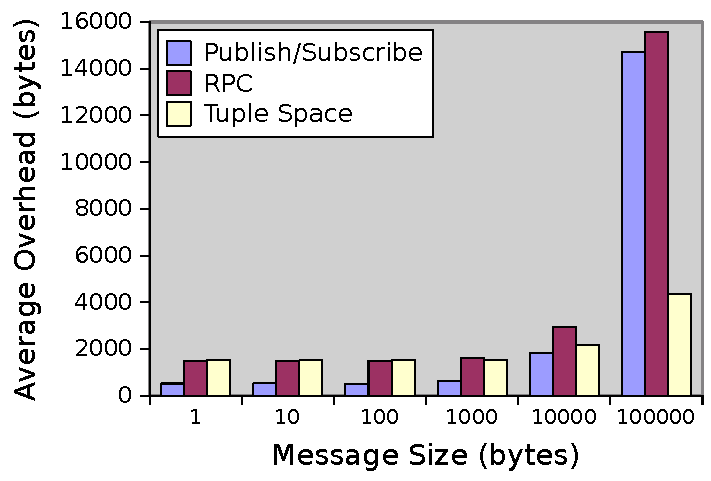
\includegraphics[width = .48\textwidth]{figures/message-overhead-bytes.pdf}
\caption{Bytes per Message}
\label{fig:overhead-bytes}
\end{figure}

\begin{figure}
\centering
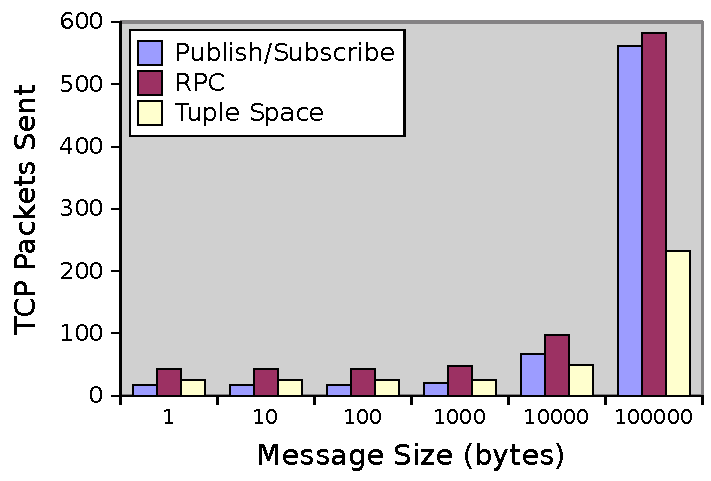
\includegraphics[width = .48\textwidth]{figures/message-overhead-packets.pdf}
\caption{TCP Packets per Message}
\label{fig:overhead-packets}
\end{figure}

\subparagraph{Network Overhead}

While Table~\ref{fig:messages} indicated the overhead added at the application layer, Figure~\ref{fig:overhead-bytes} shows the average amount of TCP traffic which is sent over the network for a single message, calculated as \textit{bytes sent} - \textit{message size}. These results use the single hop static scenario and are averaged from 50 messages.

The results are fairly constant until the packet size is exceeded. There is some increase at 10KB, and a dramatic increase at 100KB. Figure~\ref{fig:overhead-packets} shows the same data in terms of TCP packets and indicates the cause of the sharp increase in traffic at 100KB is the result of packet fragmentation.

Despite having large message sizes, tuple spaces have much lower overhead in terms of TCP traffic. This difference arises from a side issue related to TCP send window sizes. For tuple spaces, where the receiver initiates the connection, the TCP send window size grows to accommodate larger packet sizes. With RPC and publish/subscribe, the send window size remains constant, causing the large messages to be split into many more packets. For RPC and publish/subscribe, the sender initiates the TCP session, while in tuple spaces it is the receiver (of the tuple) which initiates the TCP session.

\paragraph{Message Reliability}

How reliably a communication paradigm handles message delivery has a direct impact on the application layer. The more reliable the communication paradigm, the less responsible the application is for handling lost messages. We measured reliability in terms of message delivery. In the single hop scenario, all paradigms achieved 100\% delivery and figures~\ref{fig:mgdel} and \ref{fig:mgdel} indicate nearly perfect message delivery for all the paradigms in the unicast scenario. Publish/subscribe performed the worst and still only lost 4 messages. However, this is not unexpected, since publish/subscribe sends out publications immediately, whether or not any subscribers are present.

\paragraph{Message Delay}

Message delay is another important application-level metric, as it determines how quickly information is transferred and the freshness of the application's information. Figures \ref{fig:shgps}, \ref{fig:shgrpc}, and \ref{fig:shgts} show delay in terms of round trip times for each paradigm in a single hop scenario. The majority of the messages in each paradigm are under the 200\textit{ms} mark, with just a few wayward messages taking longer. Even for tuple spaces, 80\% of the messages take less than 400\textit{ms} to complete their round trip. However, some messages take much longer, up to 8\textit{s}. For tuple spaces, this is partially due to the complexity and overhead of the messages required to perform the round trip message delivery.

However, the time delay for tuple spaces in the single hop scenario is also related to the pull (rather than push) nature of the paradigm. A tuple is time-stamped when it is output, but the tuple is not actually sent to the receiver until the receiver requests it. The same situation happens on the return trip, when the tuple must be pulled back to the original sender. Any delays in this process cause the round trip time to increase.

On the other hand, publish/subscribe messages are sent out almost immediately after being timestamped. Nearly all the delay is caused by the network itself. RPC has more potential for delays since it must find the remote method before invoking it. However, the return message can reuse the existing TCP connection, which appears to provide an advantage over tuple spaces.

The multi-hop scenario introduces more message latency, as seen in Figures \ref{fig:mhgps}, \ref{fig:mhgrpc}, and \ref{fig:mhgts}. Again, most messages complete the round trip very quickly ($<$300\textit{ms}), but the maximum times for publish/subscribe and RPC increased from 383\textit{ms} and 110\textit{ms} to 1537\textit{ms} and 902\textit{ms}, respectively. Not only does it take longer due to the packets needing to traverse multiple hops, there is also delay introduced by the time to find routes. In the single hop scenario, routes are set up at the beginning of the scenario and there is virtually zero routing activity after that. On the other hand, the multi-hop scenario performs routing updates throughout the run time of the scenario.

The mobile scenario introduces even greater delays. Routes are changing frequently and may be several hops long. While the publish/subscribe and RPC results are clustered around 100\textit{ms} and remain under 500\textit{ms}, the tuple space values are considerably higher with a median at 256\textit{ms} and a high of nearly 20\textit{s}. This is again due to the pull nature of tuple spaces and the overhead seen in Section \ref{sec:app_overhead}.

\subsubsection{Group Communication}

Group or multicast communication is a useful but more complex part of MANETs, where information and resources are often disseminated in a peer-to-peer manner. Group communication differs significantly from unicast communication. Given the mobile characteristics and decentralized nature of MANETs, a group's membership may be in constant flux, so it is unlikely a sender has perfect knowledge of the members of the group. The time difference between replies from members of the group may vary greatly, and the initiating node cannot know how many replies to expect.
%Consider an application which makes a request for some information from all nearby nodes. It is difficult to know how long it should wait to receive all replies, because it is not known how many replies should be expected, yet it is entirely possible that an application will receive multiple replies from the group. It is also possible to have a large time difference between replies from different nodes.

We have investigated how well each paradigm handled group communication by again evaluating message delay and message delivery reliability, but with multiple receivers.

\paragraph{Round Trip Application}\label{sec:rtapp}

The method for achieving group communication is slightly different for each paradigm. In publish/subscribe, there are two topics: one for outgoing messages and one for incoming messages. The sending node publishes a message containing a timestamp to the outgoing topic. When an outgoing message is received, the receiving node republishes the message to the incoming topic. The round trip time is then calculated when the sending node receives the incoming copy of the original message.

In RPC, a group method call is asynchronously invoked with a timestamp as the parameter. A group invocation will attempt to invoke all available copies of the remote method and register a callback to handle the return values. In this case, that callback will receive the original timestamp and calculate the round trip time from it.

Since tuple spaces only support pull operations, the situation is inverted. Receivers request an outgoing tuple, which will contain a timestamp. The sender outputs a proper tuple with a timestamp, which is then sent to the requesting receivers. The sender then requests a reply tuple and registers a callback to handle the tuple when it arrives. Upon receiving the tuple with a timestamp, the receiver will output a reply tuple containing the same timestamp. This tuple will be sent back to the original sender, which can then compute the round trip time. This is illustrated in Figure \ref{fig:tuple-failure}.

\begin{figure}
\centering
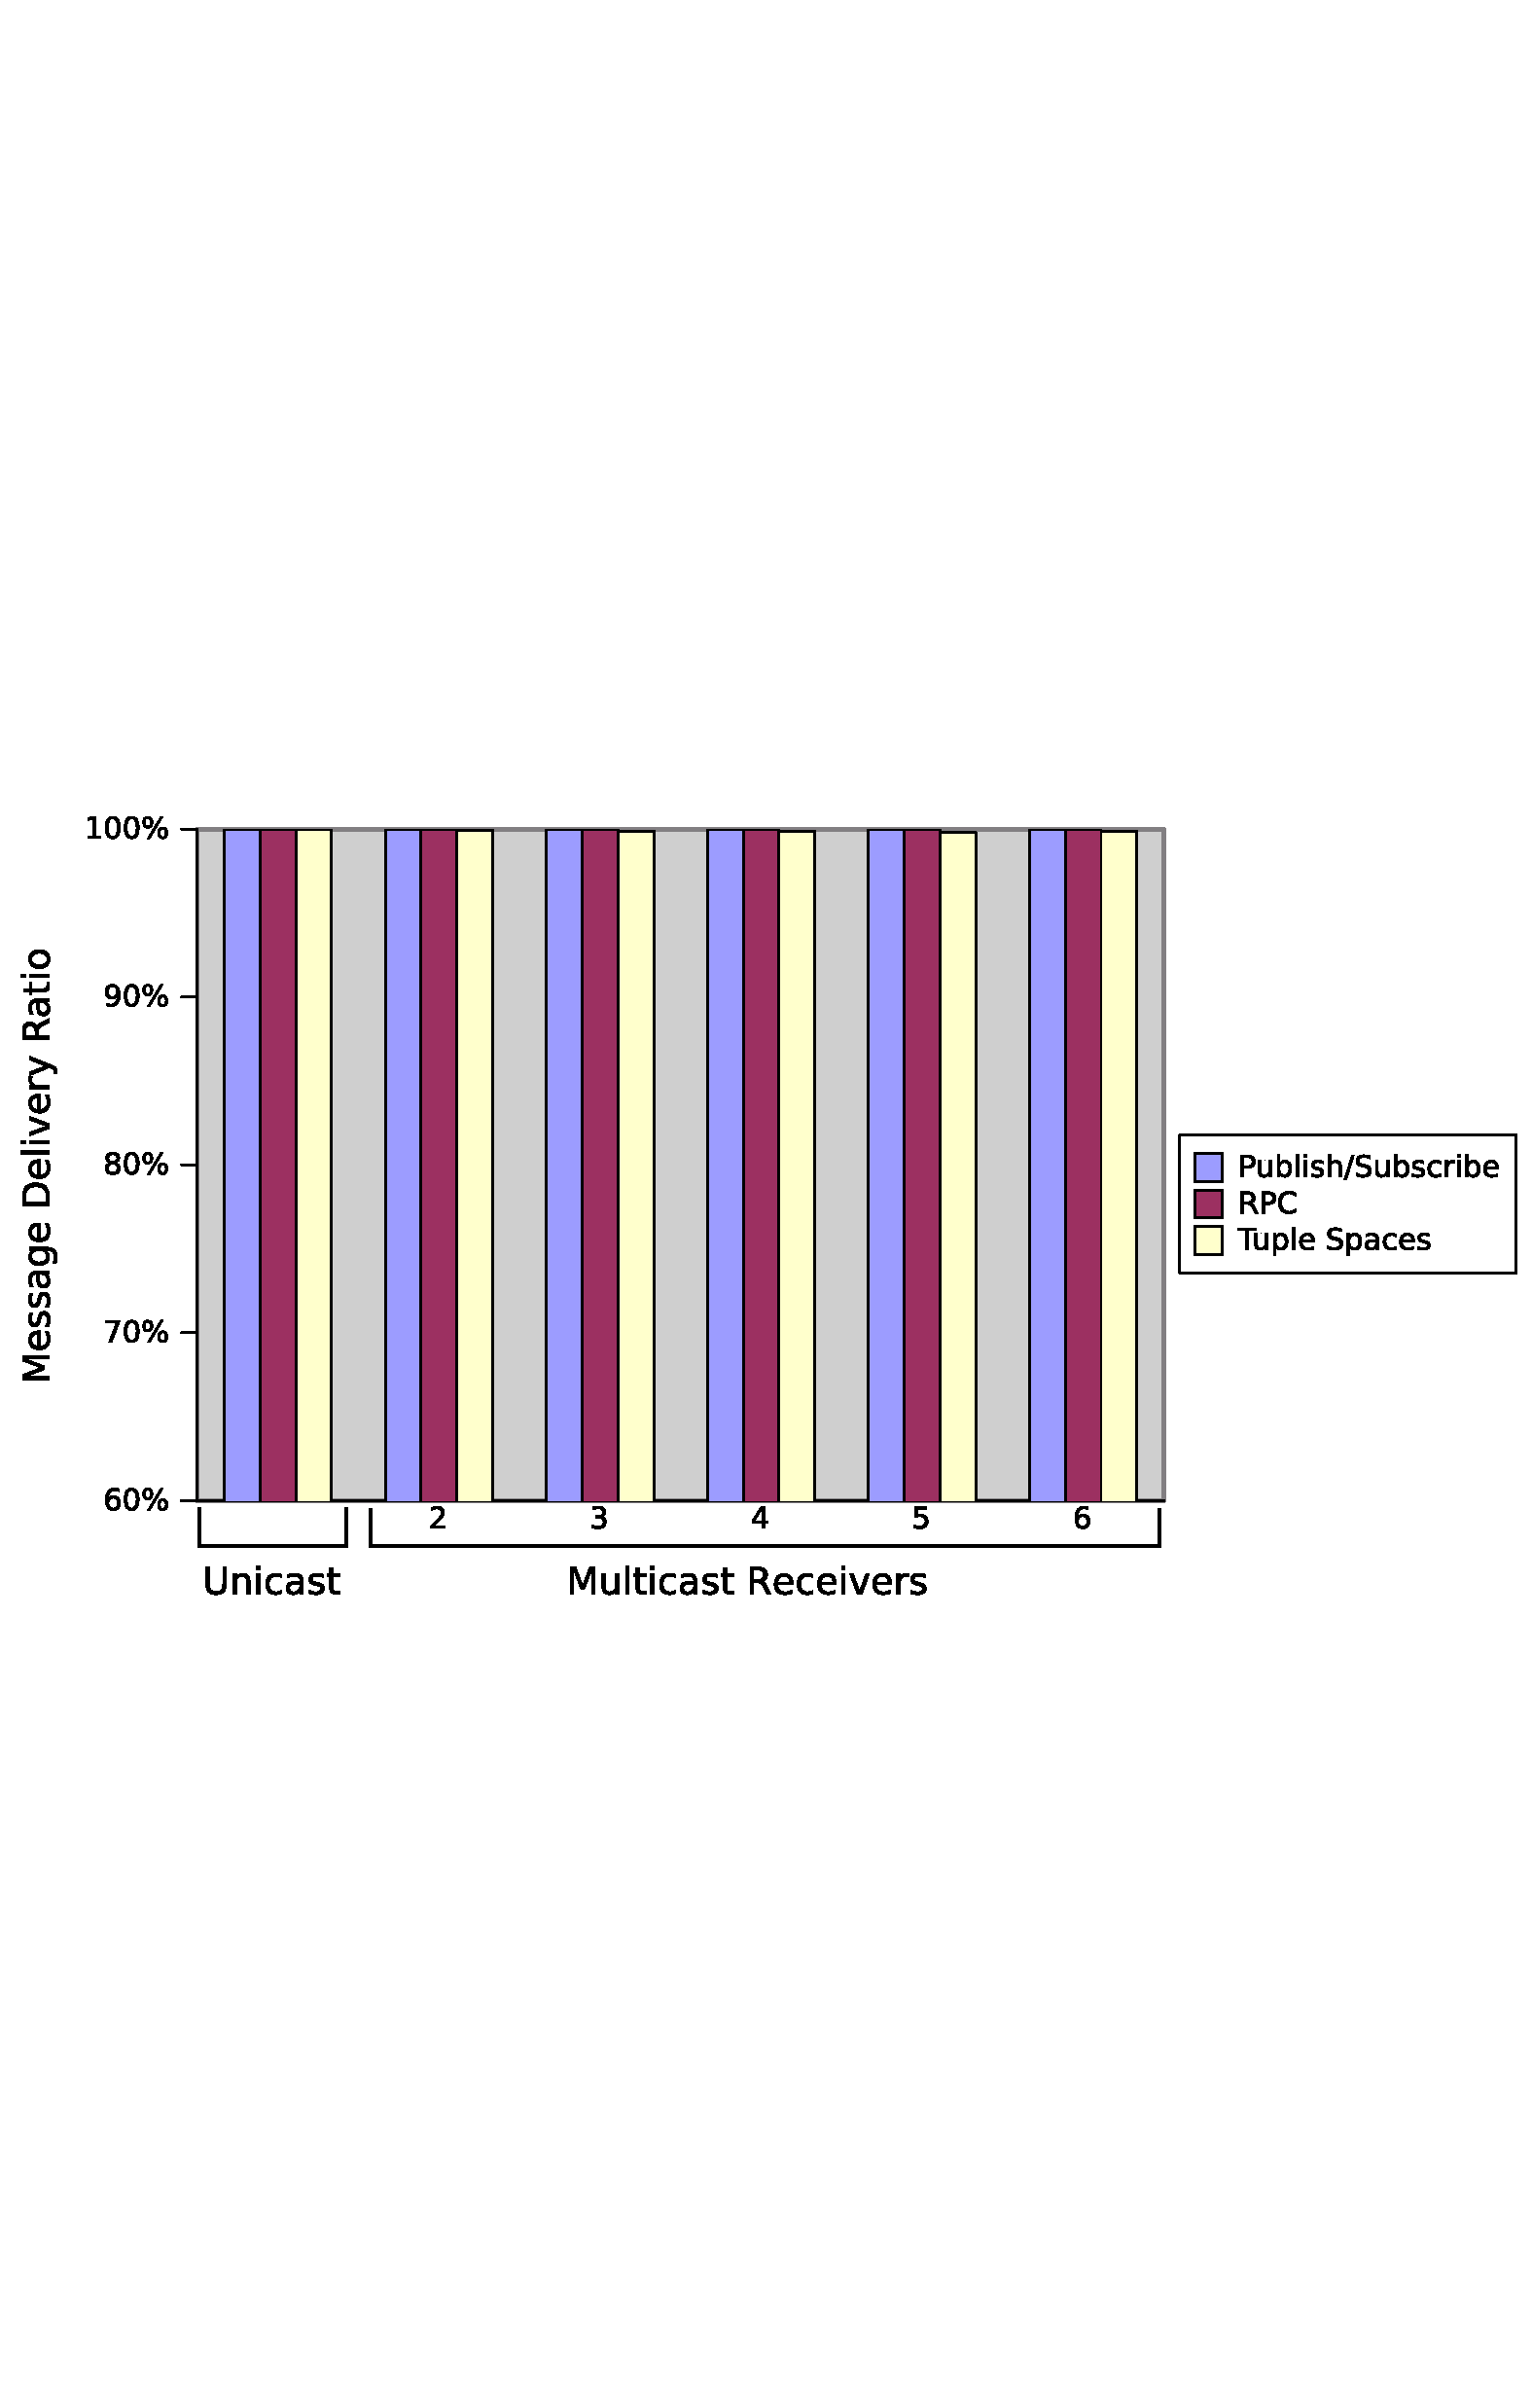
\includegraphics[width = 0.49\textwidth, clip, trim = 0px 400px 0px 400px]{figures/single-hop-group-delivery.pdf}
\caption{Message Delivery - Single Hop}
\label{fig:sgdel}
\end{figure}

\begin{figure}
\centering
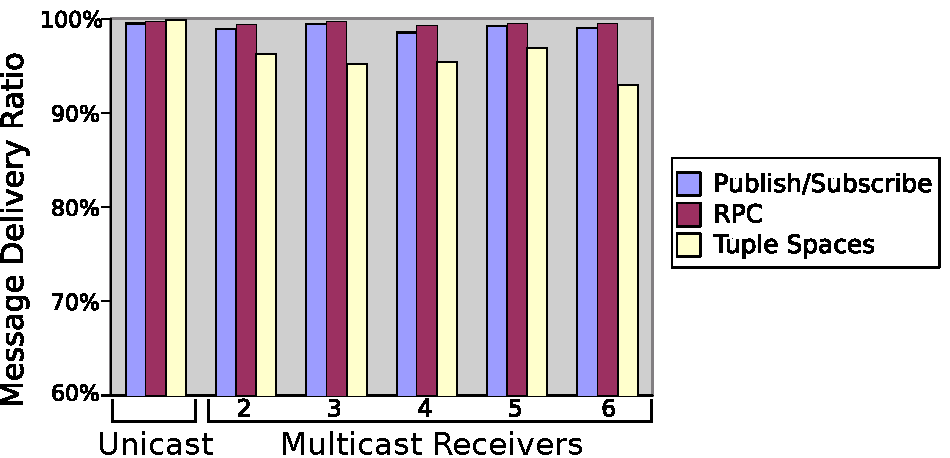
\includegraphics[width = 0.59\textwidth, clip, trim = 0px 0px 0px 0px]{figures/multi-hop-group-delivery.pdf}
\caption{Message Delivery - Multihop}
\label{fig:mhgdel}
\end{figure}

\begin{figure}
\centering
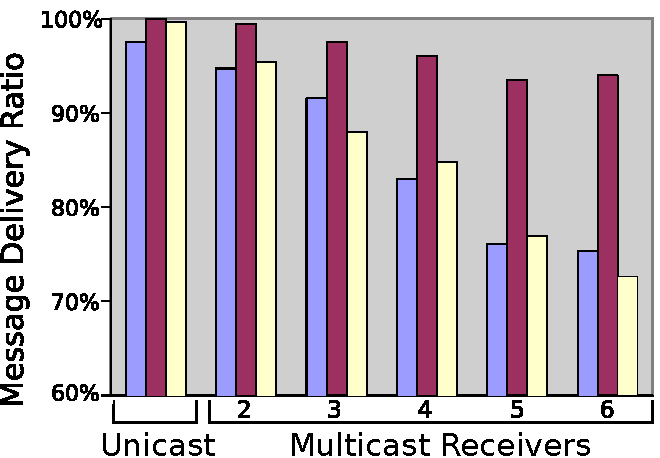
\includegraphics[width = 0.40\textwidth, clip, trim = 0px 0px 0px 0px]{figures/mobile-group-delivery.pdf}
\caption{Message Delivery - Mobile}
\label{fig:mgdel}
\end{figure}


\paragraph{Message Reliability}\label{sec:group_reliability}

With this application, message reliability refers to messages which make the circuit from the sender to the receiver and back to the sender. This is useful, for example, in situations where a sink node aggregates information from other nodes.

Figures \ref{fig:mhgdel} and \ref{fig:mgdel} show the percentage of messages successfully completing the round trip. The single hop scenario is not shown, as all paradigms achieved $>$ 99\% reliability in that scenario. In the multi-hop scenario, there are more losses even without mobility, but there is no significant trend as the number of receivers increases.

RPC has a slight advantage with this metric, as it will wait until at least one receiver is available. Publish/subscribe and tuple space will send out messages whether or not any receivers are available at the time. However, none of the communication paradigms will retry a message which is lost in transit. A message lost anywhere in the circuit causes the entire attempt to be reported as a failure. For example, if RPC is able to connect to a remote method and invoke it, but never receives a return message, it will not attempt to invoke the method again. Since these results require a message to complete the round trip circuit, there are multiple opportunities for message delivery to fail. 

This contributes to tuple spaces showing the lowest delivery ratio (93\%) in the multi-hop scenario and a low delivery ratio (72.6\%) in the mobile scenario. While tuple spaces can easily handle the delivery of the outgoing tuple, it is more difficult to guarantee the return of the reply tuple. If a node is not available to receive the request broadcast for a reply tuple, then the reply will never be sent even if the original outgoing tuple is received.

Figure \ref{fig:tuple-failure} illustrates why this is the case. The interaction in the ideal scenario assumes the sender and receiver are present for the entire interaction. In the second scenario, however, the receiver moves away from the sender after sending the initial request for an outgoing tuple. In step 3, the sender sends the reply request, but it cannot be delivered. When the receiver returns, it repeats its request for an outgoing tuple, because it is a blocking request which has not yet been satisfied. The sender satisfies the request, but the reply is never sent since the receiver never receives the reply request.

\begin{figure}
\mbox {
	\subfigure[Ideal Scenario] {
		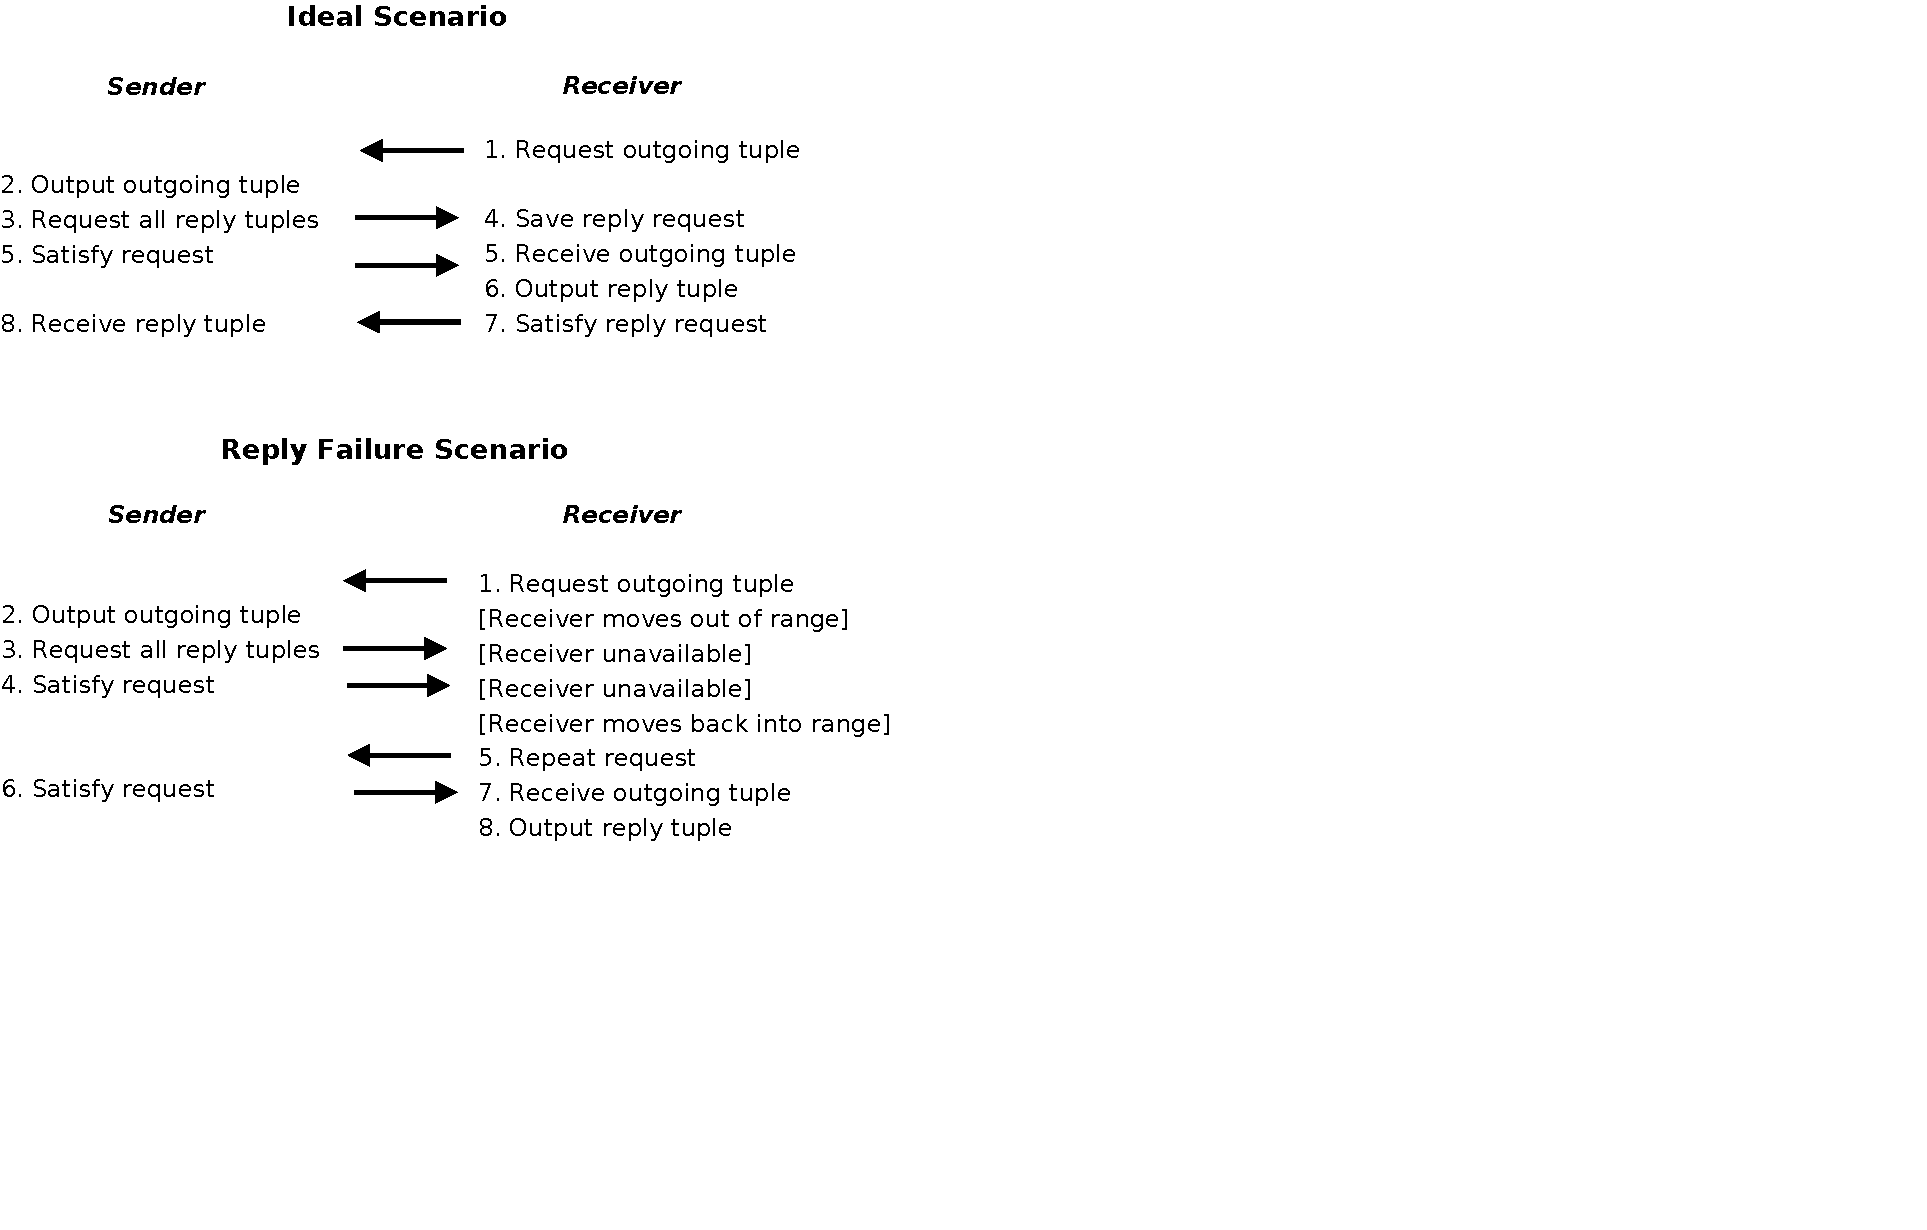
\includegraphics[scale = .40 , clip, trim = 0px 400px 500px 35px]{figures/tuple-failure.pdf}
	}
	
	\subfigure[Failure Scenario] {
		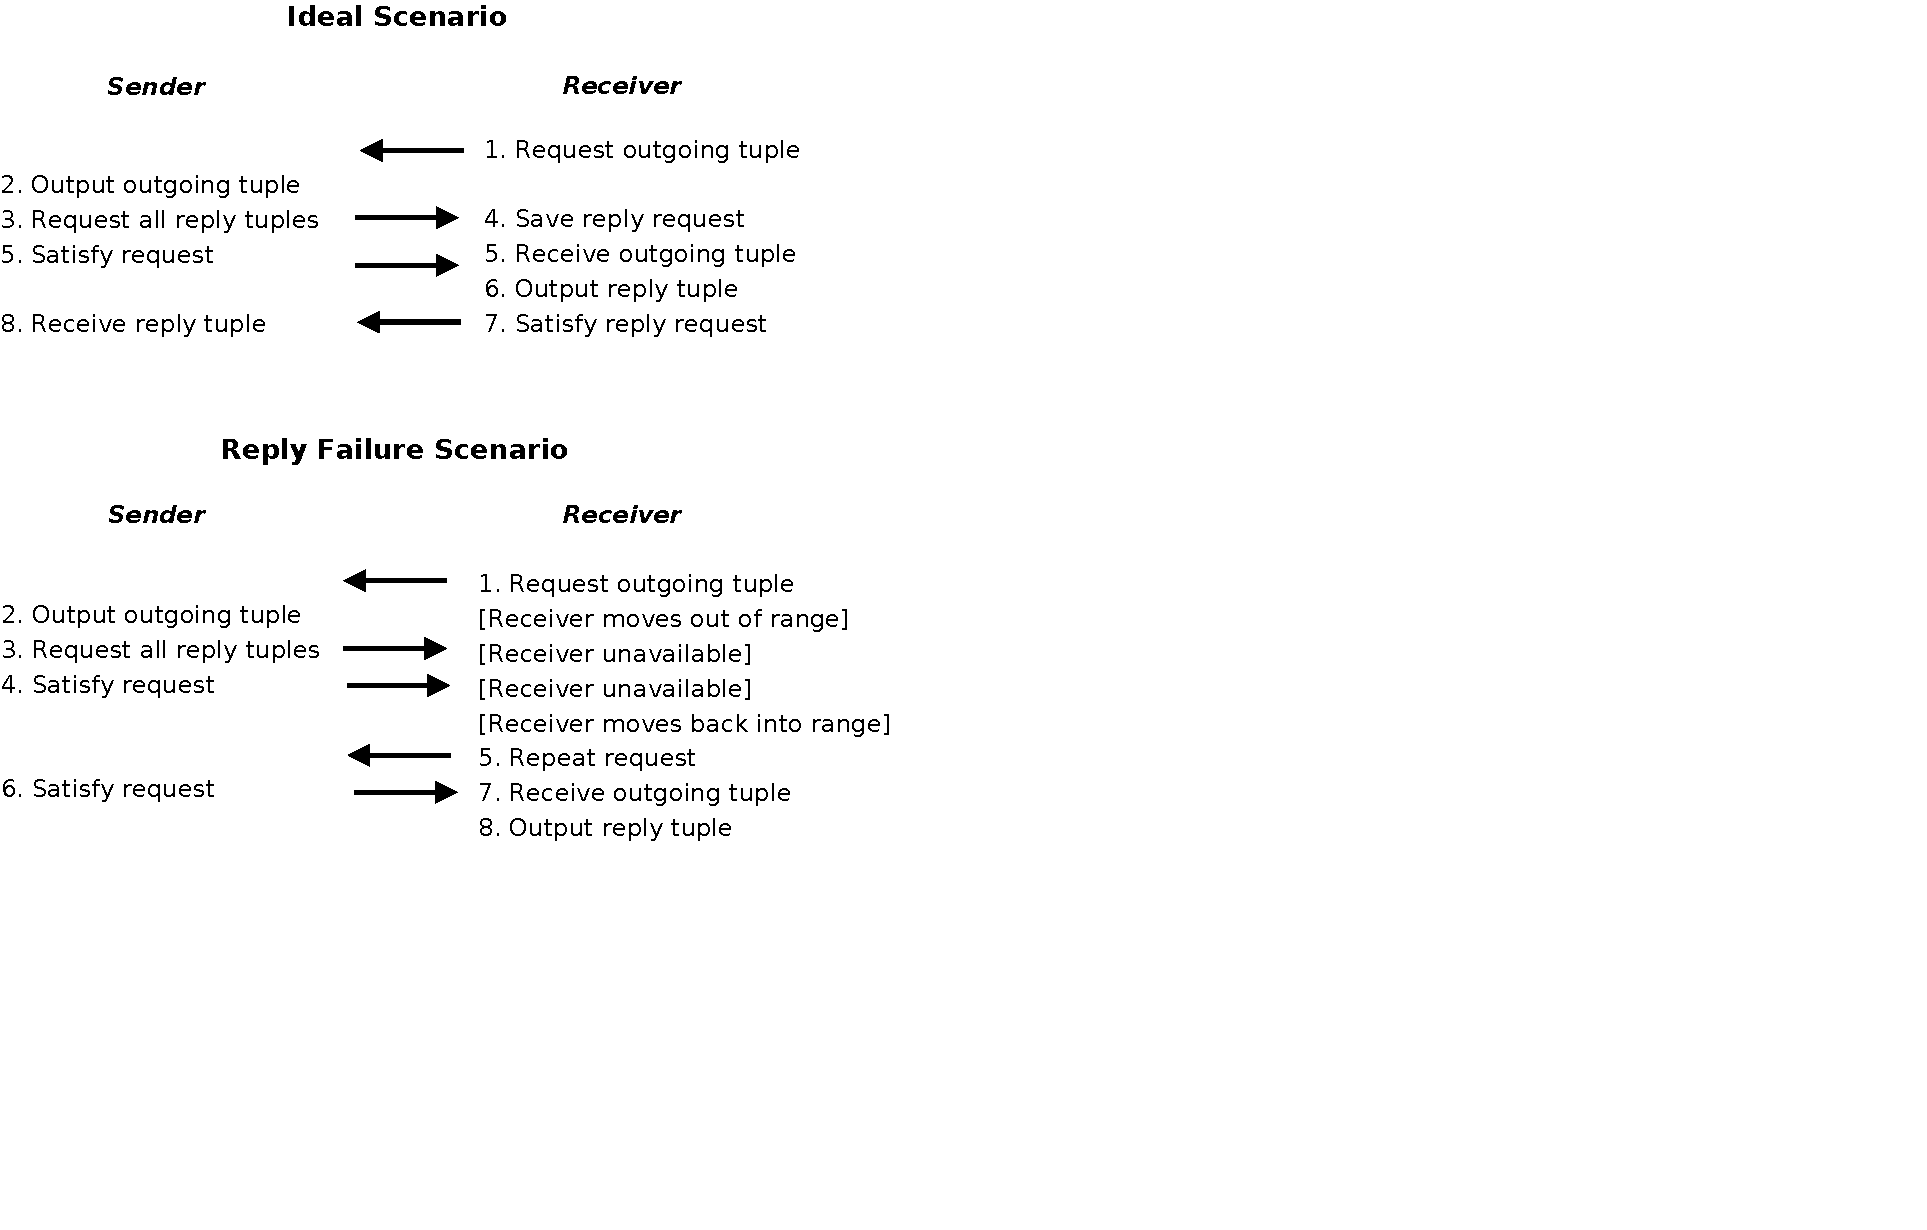
\includegraphics[scale = .40 , clip, trim = 0px 180px 450px 230px]{figures/tuple-failure.pdf}
	}
}
\caption{Tuple Space Round Trip Application}
\label{fig:tuple-failure}
\end{figure}

The solution to this situation would be to repeat the request for the reply tuples. However, the reply request is a group request. Retries are problematic for group requests, because it is unclear when a group request has been completely satisfied. While a normal \textit{rd()} \textit{or in()} operation is satisfied by a single tuple, there is no upper bound on how many tuples may be available to satisfy a group request, so the requester cannot know when to cease retrying. The LIME\cite{lime} project defines a group request as non-blocking and only operating on the current state of the tuple space. This solution would fail in \textit{both} exchanges shown in Figure \ref{fig:tuple-failure}, as the reply request may be received before the original request is satisfied. Therefore, we compromised by using blocking group requests, but without retries.

\begin{figure}
\centering
\mbox {
	\subfigure[Publish/Subscribe - Single Hop] {\label{fig:shgps}
	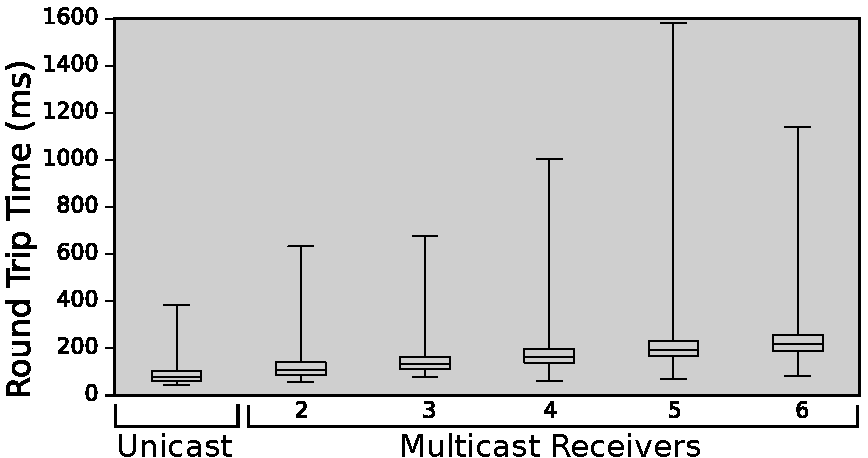
\includegraphics[width = .49\textwidth]{figures/single-hop-group-ps.pdf}
	}

	\subfigure[Publish/Subscribe - Multi-hop] {\label{fig:mhgps}
	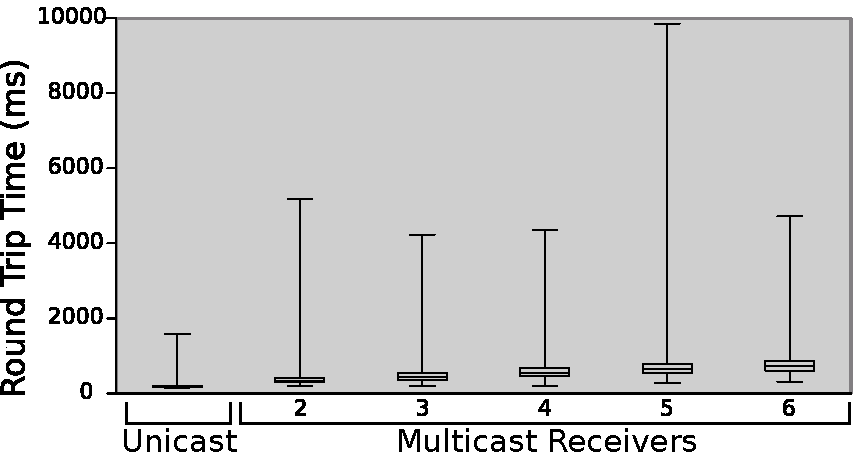
\includegraphics[width = .49\textwidth]{figures/multi-hop-group-ps.pdf}
	}
}
\mbox {
	\subfigure[RPC - Single Hop] {\label{fig:shgrpc}
	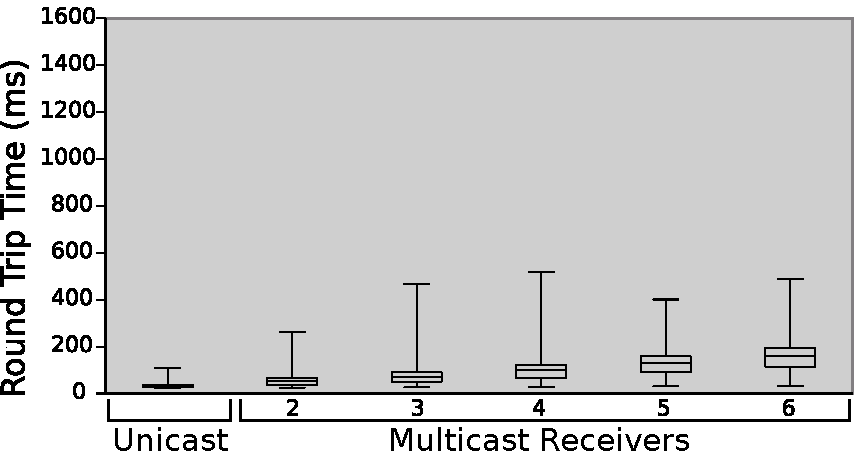
\includegraphics[width = .49\textwidth]{figures/single-hop-group-rpc.pdf}
	}
	
	\subfigure[RPC - Multi-hop] {\label{fig:mhgrpc}
	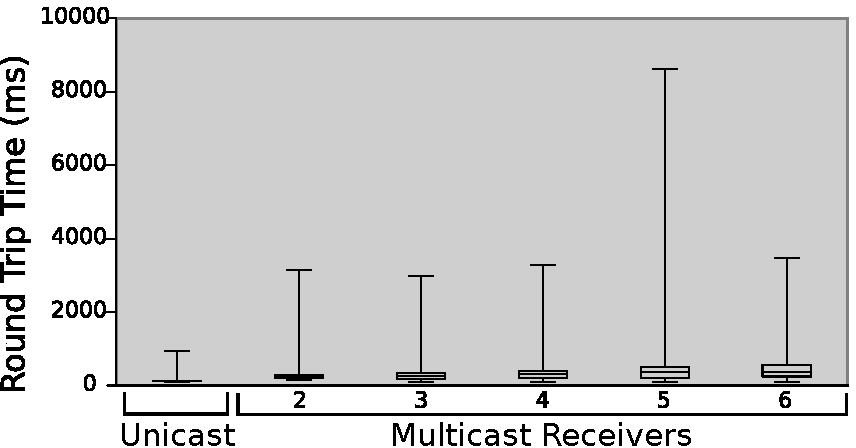
\includegraphics[width = .49\textwidth]{figures/multi-hop-group-rpc.pdf}
	}
}
\mbox {

	\subfigure[Tuple Space - Single Hop] {\label{fig:shgts}
	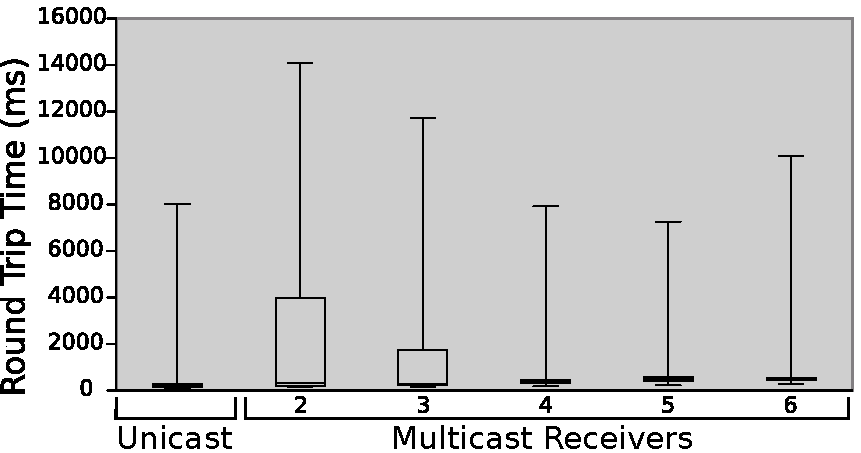
\includegraphics[width = .49\textwidth]{figures/single-hop-group-ts.pdf}
	}

	\subfigure[Tuple Space - Multi-hop] {\label{fig:mhgts}
	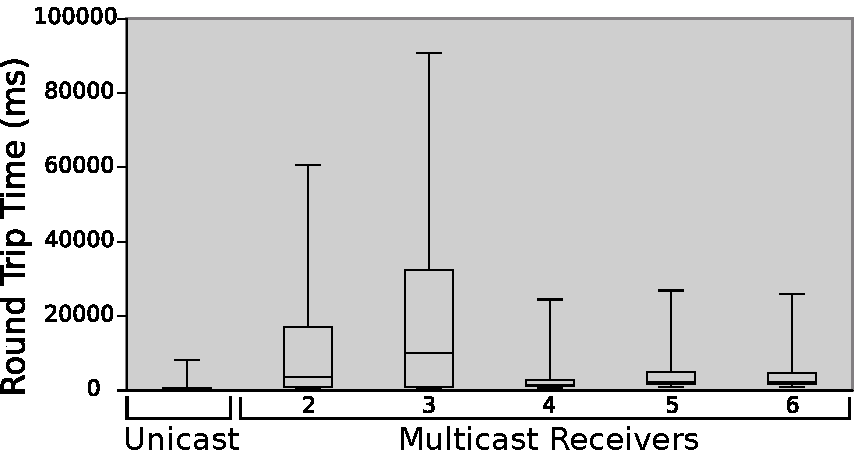
\includegraphics[width = .49\textwidth]{figures/multi-hop-group-ts.pdf}
	}
}
\mbox {
	\subfigure[Publish/Subscribe - Mobile] {\label{fig:mgps}
	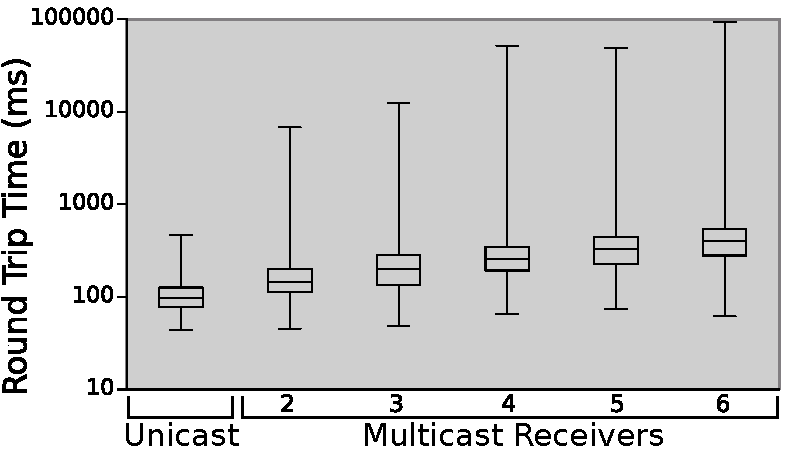
\includegraphics[width = .49\textwidth]{figures/mobile-group-ps.pdf}
	}
	
	\subfigure[RPC - Mobile] {\label{fig:mgrpc}
	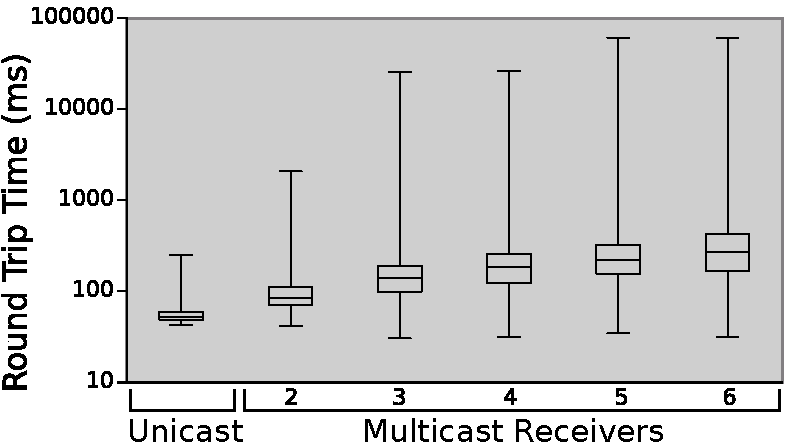
\includegraphics[width = .49\textwidth]{figures/mobile-group-rpc.pdf}
	}
}
	\subfigure[Tuple Space - Mobile] {\label{fig:mgts}
	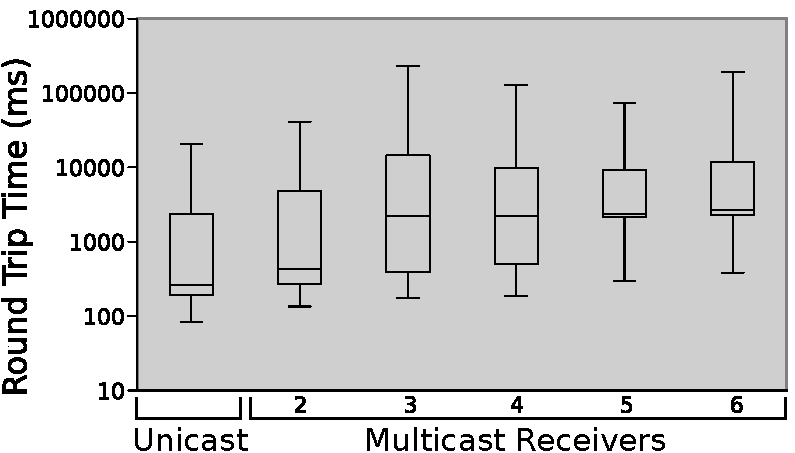
\includegraphics[width = .49\textwidth]{figures/mobile-group-ts.pdf}
	}

\caption{Round Trip Times}
\end{figure}

\paragraph{Message Delay}\label{sec:group_delay}

We again consider round trip time for each of the paradigms, but this time with an increasing number of receivers. Figures \ref{fig:shgps} - \ref{fig:mgts} show the results for each paradigm and scenario.

For the single hop and multi-hop scenarios, where there is no mobility, the majority of the round trip times are fairly fast. The bottom 75\% of the messages have very similar results, while the top 25\% varies much more. This indicates that an application can expect most messages to be delivered quickly or not at all, but about a quarter of the messages may arrive up to minutes later.

The median delay does increase as receivers are added, especially in the mobile scenario. In the static scenario, the median delay publish/subscribe increased 121\textit{ms} from two receivers to six receivers. RPC increased 147\textit{ms}, and tuple spaces increased 140\textit{ms}. For the mobile scenario, the median times for publish/subscribe increased 255\textit{ms}, RPC increased 237\textit{ms}, and tuple spaces increased by 2035\textit{ms}. The maximum delay values varied much less predictably. For tuple spaces, the static scenarios have unusually long delays with two and three receivers. In the static scenarios, the first three receivers are located in close proximity. One node would dominate the channel for several seconds before relinquishing it. Once again, this shows how influential the wireless channel is on the performance and behavior of applications in MANETs.

The median and maximum tuple space results are much longer than the other two paradigms. The median delay for tuple spaces ranges from twice as much as publish/subscribe in the single hop scenario up to 6 times as high in the mobile scenario. For publish/subscribe and RPC, the majority of delays can only be caused by the network, since they do not attempt to retransmit messages. Tuple spaces, on the other hand, can have very large delays due to the paradigm itself. Note that steps 1 and 2 in Figure \ref{fig:tuple-failure} can be reversed: the outgoing tuple can be timestamped before it is even requested by the receiver.

If a receiver is ``behind" it may spend time receiving older tuples before the newest tuple is requested. This causes the round trip times to increase while only improving one-way message delivery. While it does improve one-way message delivery, it does not improve the round trip message delivery ratio, due to the reasons discussed in Section \ref{sec:group_reliability}.

\subsubsection{Shared Whiteboard Application}

When testing the whiteboard application, we considered the metrics which a user might care about at the application level: how reliably and quickly users receive updates.
This models a classroom or presentation setting where the instructor or presenter is the only one writing on the shared whiteboard, but the contents of the whiteboard are shared out to the class or audience. As in the group communication experiments, in each scenario Node 1 is the sender, with the other nodes marked with triangles as the receivers.
In the results below, a single user is updating the whiteboard and the updates are propagated to 6 receivers. We used traffic traces from  Coccinella\footnotemark to ensure our implementation accurately represented a typical whiteboard application. For these experiments, 250 whiteboard update messages of varying sizes were sent out over a 10 minute period at varying intervals.

\footnotetext{http://thecoccinella.org/}

Furthermore, we tested the whiteboard application under the two different routing protocols we have been using, AODV and DSR. This is not meant to be an exhaustive comparison of the routing protocols themselves, but is intended to show how the choice in routing protocols might affect the performance of the communication models in a nontrivial application.

\begin{figure}
\centering
\mbox {
	\subfigure[DSR] {\label{fig:wbdeliverydsr}
	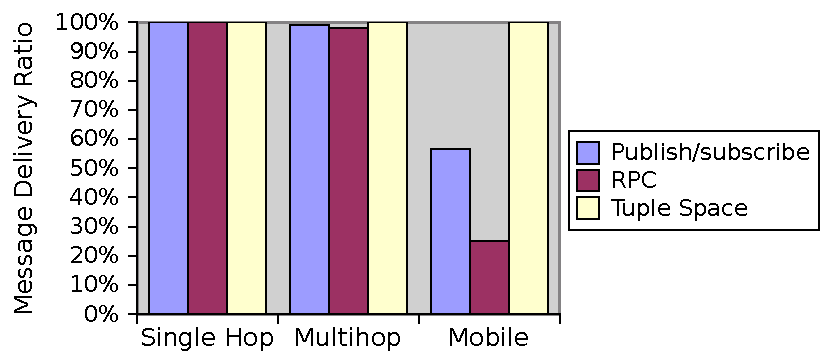
\includegraphics[width = .55\textwidth, clip, trim = 6px 0px 4px 0px]{figures/wb-dsr-delivery.pdf}
	}

	\subfigure[AODV] {\label{fig:wbdeliveryaodv}
	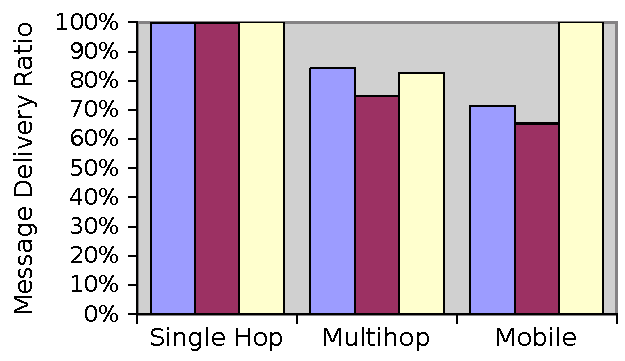
\includegraphics[width = .41\textwidth, clip, trim = 6px 0px 2px 0px]{figures/wb-aodv-delivery.pdf}
	}
}
\caption{Whiteboard Message Delivery}
\end{figure}

\paragraph{Message Reliability}

Unlike the previous results, these represent one-way communication from the whiteboard user to the receivers. Message reliability determines how accurately the receivers' views reflect the state of the shared whiteboard.

Figures~\ref{fig:wbdeliverydsr} and ~\ref{fig:wbdeliveryaodv} show the percentage of whiteboard messages delivered for DSR and AODV, respectively. As before, the results are nearly 100\% for all paradigms and both protocols in the single hop network. AODV performs poorly on the multi-hop scenario, while DSR achieves nearly 100\% delivery for all paradigms. On the other hand, DSR performs much worse in the mobile scenario, with the delivery ratio for RPC only reaching 25\%.

The reliability of tuple spaces is considerably better in these experiments than in the round trip scenario, with 100\% delivery in all but the AODV multi-hop scenario. The difference between these results and Section \ref{sec:group_reliability} is the lack of a return message. Each receiver is responsible for requesting the whiteboard updates, so the blocking request will be retried until the tuples are received. The only exception is the multi-hop scenario with AODV, in which all three paradigms perform much worse. Since all three paradigms are affected equally, these results must be directly due to the behavior of AODV in this scenario. Investigation of this phenomenon is outside the scope of this paper.

While the choice of routing protocol can have a significant effect on the paradigm performance, it appears to affect each paradigm in the same manner. In other words, neither routing protocol improves the performance of one paradigm while causing a different paradigm to perform worse.

\begin{figure}
\centering

\mbox {
	\subfigure[DSR] {\label{fig:wbdelaydsr}
	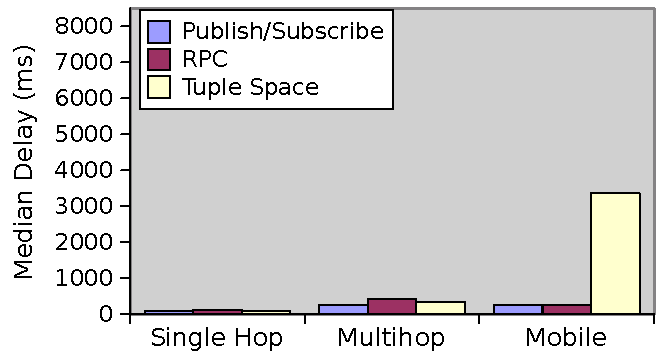
\includegraphics[width = .49\textwidth, clip, trim = 6px 0px 4px 3px]{figures/wb-dsr-delay.pdf}
	}

	\subfigure[AODV] {\label{fig:wbdelayaodv}
	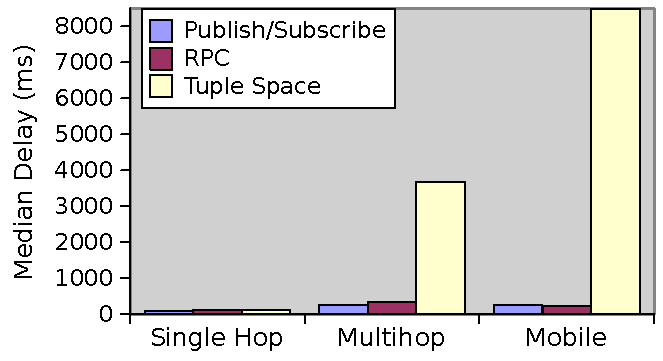
\includegraphics[width = .49\textwidth, clip, trim = 6px 0px 2px 3px]{figures/wb-aodv-delay.pdf}
	}
}
\caption{Whiteboard Message Delay}
\end{figure}


\paragraph{Message Delay}

Message delay is measured as the time from when a whiteboard update is sent by the application until it is delivered to the receiver's whiteboard. Update delays are very noticeable in a shared whiteboard application, so the delay time should be minimized.

Figure~\ref{fig:wbdelaydsr} shows the results when using DSR and Figure~\ref{fig:wbdelayaodv} shows the AODV results. Not unexpectedly, tuple spaces have the highest median latencies of 8,486\textit{ms} with AODV and 3,357\textit{ms} with DSR. For publish/subscribe and RPC, the median delay remained under 400\textit{ms}. As noted previously, there is an obvious direct relationship between reliability and the message delay time. If a message cannot be delivered immediately, the communication paradigm can either drop the message or retry later. Dropping the message decreases reliability, but the median message delay will be low. However, attempting to deliver the message later increases both reliability and message delay.

With DSR, tuple spaces report a nearly 100\% delivery ratio in every scenario, yet the delay times are $<$400\textit{ms} in the static scenarios. In contrast, AODV causes long delays for tuple spaces in both the multi-hop and mobile scenarios. Since tuple spaces will repeatedly attempt to deliver messages, retries are expected to contribute to the majority of the delays. This is supported by the long delay times experienced by tuple spaces with AODV in the multi-hop scenario. However, in the mobile scenario tuple spaces achieve 100\% delivery with AODV and DSR, but the median delay with DSR is less than half as with AODV.

From the mobile reliability results, we can infer that DSR does not maintain viable routes, because the results of publish/subscribe and RPC are poor. However, the delay results suggest DSR is faster than AODV at finding new routes when they become available.


\subsubsection{Routing Overhead}\label{sec:routing}

\begin{figure}
\centering
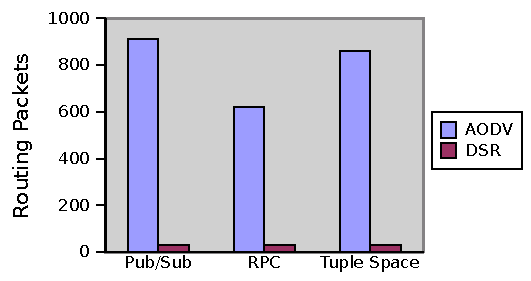
\includegraphics[scale = .75]{figures/single-hop-routing.pdf}
\caption{Whiteboard Routing Overhead - Single Hop}
\label{fig:wbrouting-sh}
\end{figure}

\begin{figure}
\centering
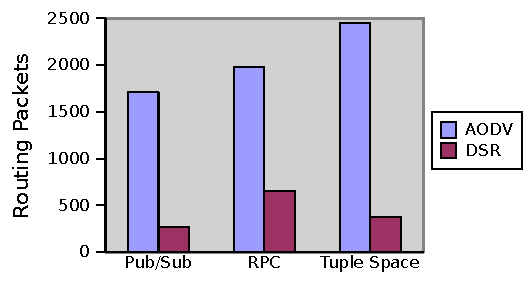
\includegraphics[scale = .75]{figures/multi-hop-routing.pdf}
\caption{Whiteboard Routing Overhead - Multihop}
\label{fig:wbrouting-mh}
\end{figure}

\begin{figure}
\centering
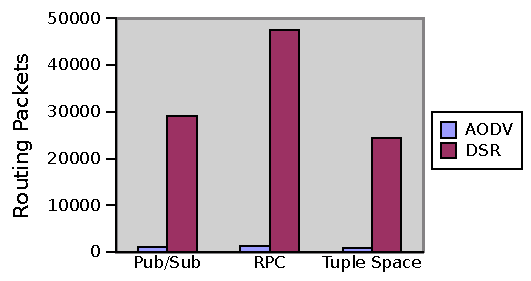
\includegraphics[scale = .75]{figures/mobile-routing.pdf}
\caption{Whiteboard Routing Overhead - Mobile}
\label{fig:wbrouting-m}
\end{figure}

Above, we investigated application and transport layer overhead for each paradigm. In this section, we look at the routing overhead incurred for each paradigm when used in the whiteboard application. Ideally, the amount of routing overhead should be as small as possible in order to conserve bandwidth.

Figures \ref{fig:wbrouting-sh}, \ref{fig:wbrouting-mh}, and \ref{fig:wbrouting-m} show the number of routing packets generated in each scenario. For the single hop and multihop scenarios, DSR has much lower overhead. Once mobility is introduced, however, the routing packets from DSR dwarf the number used by AODV. This appears to correspond to the low message delivery in Figure \ref{fig:wbdeliverydsr}, although the message delay remains low for the messages which are actually delivered.

From these results, no clear correlation can be drawn between the paradigms and the amount of routing overhead. It varies according to both the network scenario and which routing protocol is used.


\chapter{MELON Coordination Model}\label{chapter:model}

MELON\footnote{Message Exchange Language Over the Network} is a practical approach for distributed communication in MANET applications that provides persistent messages, reliable FIFO-ordered multicast, efficient bulk retrieval, and simple message streaming. MELON is intended to be a general purpose MANET communication paradigm, as opposed to focusing on a specific use case such as context-aware applications, pervasive computing, or sensor networks. 

\section{Design Overview}

The design of MELON is centered around a distributed shared message store. Each device in the network may host any number of applications which access and contribute to the shared message store. Each application hosts a local message store which may be accessed by any other local or remote application. Applications request messages (which may be stored locally or remotely) using message templates.

By communicating through a shared message store, the concept of a connection between hosts is eliminated and thus disconnections are no longer an issue at the application layer. A host suddenly leaving the network does not disrupt an application and applications do not need to handle a communication operation returning an error or failing due to intermittent network connectivity or physical wireless interference. The application is effectively insulated from these issues by the nature of the paradigm and the semantics of the operations.

Since messages are exchanged through a shared message store, messages are sent and received asynchronously with no need for a persistent connection. This provides temporal decoupling between hosts, since messages can still be delivered even after prolonged disconnections.

Due to the dynamic network topology of MANETs, maintaining any type of logical or overlay network structure becomes challenging, so MELON does not rely on a particular network structure. Discovery of available messages is performed dynamically for each operation. While this does increase the amount of communication required for each operation, it removes the need for global state and allows the network to change at any time.

MELON also provides spatial decoupling (where the sender and receiver need not be aware of each other) by matching messages based on content, rather than by a host address or location. The messages themselves may physically reside on any host in the network. The sender of a message is not aware of the receivers' identities nor even how many receivers might read a message. This frees applications from tracking remote addresses or contacting a directory service to find remote resources.

The shared wireless communication medium in MANETs is well-suited to group or multicast communications. MELON supports multicast communication by allowing any number of receivers to read the same message. MELON also provides bulk receives, which allow applications to efficiently receive multiple messages from multiple hosts in a single operation.

Applications often require point-to-point or unicast communication as well. While unicast communication can be accomplished through by storing regular messages in MELON, this communication can easily be disrupted by a process removing a message intended for a different receiver. Additionally, it is possible to eavesdrop on messages unnoticed by reading a message and not removing it. For applications such as instant messaging, it is important to have private unicast communication. In MELON, messages may be directed to a specific receiver when stored to ensure the messages are only taken by the intended recipient.

MELON also includes features uncommon to shared message stores to further simplify application development in MANETs. First, messages are returned in first-in first-out order per host. When a host receives a message request, it returns the oldest matching message in its local storage. In applications where a single host generates the majority of the messages, this eliminates the need to order messages on the receiver side.

Secondly, MELON provides operations to only read messages which were not previously read by the same process. This enables an application to read all matching messages currently in the message store, then read only newly-added messages in subsequent operations. It also prevents an application from reading the same message twice.

Lastly, MELON differentiates between messages which are meant to persist and be read by many receivers versus messages intended to be removed from the message store. For example, messages in a news feed would have many readers, but the messages themselves should not be removed. On the other hand, a job queue expects each job to be removed by exactly one worker. MELON provides operations to support both of these scenarios.

\section{MELON Operations Overview}

\begin{table}
\centering
\caption{Operations Summary}
\begin{tabular}{|c|c|c|c|} \hline
& Add single message & Retrieve single message & Retrieve many messages \\ \hline
Nondestructive retrieval & \textbf{write} & \textbf{read} & \textbf{read\_all} \\ \hline
Destructive retrieval & \textbf{store} & \textbf{take} & \textbf{take\_all} \\ \hline
\end{tabular}
\label{table:opsummary}
\end{table}

Messages can be copied to the shared message store via a \textbf{store} or \textbf{write} operation. A \textbf{store} operation allows the message to later be removed from the storage space. Messages saved with a \textbf{write} operation cannot be explicitly removed from the storage space, only copied.

Messages added via \textbf{store} may be retrieved by a \textbf{take} operation using a message template which specifies the content of the message to be returned. A \textbf{take} operation will remove a message with matching content from the message store and return it to the requesting process. \textbf{take} operations are atomic: a message may only ever be returned by a single \textbf{take} operation.

A \textbf{read} operation will also return a message matching a given template, but does not remove the original message from the shared storage. Any number of processes may read the same message. However, repeated applications of a \textbf{read} operation in the same process will never return the same message. Only messages stored with \textbf{write} can be returned by a \textbf{read} operation.

The basic \textbf{take} and \textbf{read} operations return a single message per invocation. To facilitate the exchange of multiple messages, MELON includes the bulk operations \textbf{take\_all} and \textbf{read\_all}. The bulk versions operate the same as the basic operations, except all available matching messages will be returned instead of a single message. For \textbf{read\_all}, only messages which were not previously returned by a \textbf{read} or \textbf{read\_all} in the same process will be returned.

By default \textbf{take}, \textbf{take\_all}, \textbf{read}, and \textbf{read\_all} will block the process until a matching message is available. MELON also provides non-blocking versions of these operations. The non-blocking operations will return a null value if no matching messages can be found.

When a message is saved with a \textbf{store} operation, it may optionally be directed to a specific receiver. In a directed message, the identity of a receiver is included in the message as the addressee. Only the addressee may access a directed message through a \textbf{take}.

Due to the limited resources of most devices in a mobile network, storage space in MELON is explicitly bounded. Any message may be garbage collected prior to being removed by a \textbf{take} if capacity is reached.

\subsection{Operation Details}

Processes in MELON communicate by storing messages to a distributed shared message store and retrieving the messages based on templates. In this paper, we assume messages consist of an ordered list of typed values and optionally an addressee. However, nothing in the paradigm itself limits how messages might be constructed (e.g., they could be an unordered tuple with named values instead).

A message template is similar to a message, except it may contain both values and types. For example, a message containing \texttt{[1, "hello"]} could be matched by a template containing \texttt{[1, String]} or \texttt{[Integer, "hello"]} or \texttt{[Integer, String]}. A type will also match any subtypes.

Each operation is implemented as a separate function call. \textbf{store} and \textbf{write} operations have null return values and return as soon as the saved message is available in the message store. \textbf{take} and \textbf{read} operations block by default until a matching message is returned, but may be set to non-blocking on a per-call basis.

\begin{table}
\centering
\begin{tabular}{|c|c|}
\hline
\textbf{Operation} & \textbf{Return Type} \\ \hline
\textbf{store}(\textit{message}, \textit{[address]}) & \textit{null} \\ \hline
\textbf{write}(\textit{message}) & \textit{null} \\ \hline
\textbf{take}(\textit{template}, \textit{[block = true]}) & \textit{message} or \textit{null} \\ \hline
\textbf{read}(\textit{template}, \textit{[block = true]}) & \textit{message} or \textit{null} \\ \hline
\textbf{take\_all}(\textit{template}, \textit{[block = true]}) & \textit{array} \\ \hline
\textbf{read\_all}(\textit{template}, \textit{[block = true]}) & \textit{array} \\ \hline
\end{tabular}
\caption{MELON Operations}
\end{table}

The \textbf{store} operation takes a message as an argument and optionally an address. When called, \textbf{store} saves a copy of the message in the message store. Messages saved with \textbf{store} may only be retrieved with a \textbf{take} or \textbf{take\_all} operation. If an address is provided, then only the host with a matching identity can remove the message. Since storage space is bounded, messages may be automatically garbage collected from the storage space prior to explicit removal by a \textbf{take} or \textbf{take\_all} operation.

The \textbf{write} operation also stores a single message in the message store, but the message may only be copied from the storage space with a \textbf{read} operation, never explicitly removed. Messages written with the \textbf{write} operation may be automatically garbage collected.

A \textbf{take} operation requires a message template as the first argument and an optional boolean for the second argument.

The message template is matched against available messages in the message store which were added with a \textbf{store} operation. If a matching message is found, it will be removed from the message store and returned.

The block argument, which defaults to true if no argument is given, controls behavior of the operation if no matching message is available. If \textit{block} is true, the operation will wait until a matching message is available, then return it. If \textit{block} is false, the operation will return a null value.

Once a message has been returned by a \textbf{take} operation, it is removed from the message store and may not be returned by a subsequent operation in any process.

The \textbf{read} operation accepts the same arguments as \textbf{take}. A \textbf{read} operation will only return messages stored with a \textbf{write} operation which have not already been read by the current process.

If a message matching the given message template is available, it will be copied and returned, but not removed from the message store. Once a message has been returned to a process, the message is considered to have been read by that process and will not be returned by any subsequent read or read\_all operations in the same process.

When a matching unread message is not available, behavior of \textbf{read} depends on the \textit{block} argument. If the argument is true or unspecified, the operation will block until a matching message is available, then return that message. If the argument is false, the operation will return a null value.

A message may be \textbf{read} by any number of processes, but each process may only read each messages at most once.

\begin{table}
\centering
\caption{Read from multiple processes}
\begin{tabular}{|c|c|c|} \hline
\textbf{Process A} & \textbf{Process B} & \textbf{Process C} \\ \hline
\texttt{write([1, "hello"])} & \texttt{m = read([Integer, String])} & \texttt{m = read([Integer, String])} \\ \hline
\end{tabular}
\label{fig:readprocesses}
\end{table}

Table \ref{fig:readprocesses} illustrates one process writing a single message containing the integer \texttt{1} and the string \texttt{"hello"}. Processes B and C each perform a \textbf{read} operation with the template \texttt{[Integer, String]} which matches the message stored by process A. Since \textbf{read} does not modify the storage space, the value of \textit{m} for both process B and C will be a copy of the message \texttt{[1, "hello"]} from Process A.

The \textbf{take\_all} operation performs a bulk \textbf{take} on the given message template. The return value of \textbf{take\_all} is an array of matching messages. As with \textbf{take}, messages returned by a \textbf{take\_all} are removed from the shared storage and may not be returned by any subsequent operation in any process. A \textbf{take\_all} operation will not return a directed message unless the addressee matches the current process. Only messages stored by a \textbf{store} operation will be returned by \textbf{take\_all}.

When there are no matching messages and the value of \textit{block} is \textit{true} or unspecified, the operation will block until at least one matching message is available and then return an array of available messages. If \textit{block} is \textit{false}, \textbf{take\_all} will return an empty array.

\textbf{read\_all} performs a bulk read on the given message template and returns an array of matched messages. \textbf{read\_all} only returns messages which have not been previously returned in the same process by a read or \textbf{read\_all}. A \textbf{read\_all} operation will only return messages written by a \textbf{write} operation.

When there are no matching messages and the value of \textit{block} is true or unspecified, the operation will block until at least one matching message is available and return an array of available messages. If \textit{block} is false \textbf{read\_all} will return an empty array.

\section{Message Store Model}

MELON's operates through a semi-persistent shared message store. The message store must match message templates to actual messages, provide concurrent access for multiple clients, manage returning messages in per-host FIFO order, implement basic access control as required by MELON operations, and of course be reasonably fast.

MELON's message store is only \textit{semi}-persistent because it does not attempt to reliably retain all stored messages, and because the MELON paradigm explicitly acknowledges space limitations on mobile devices and will perform garbage collection of messages if necessary to store newer messages. Given the turbulent nature of MANETs, it is not practical for the message store to reliably retain all messages. Nodes will unexpectedly disconnect from the network, taking with them any hosted messages. If some global data structure were used for the message store, nodes moving from one network to another would need to explicitly disconnect from one shared message store, then explicitly join the next. This is not a practical constraint with the fluid and unpredictable nature of MANETs.

From the perspective of an application, the message store is a single entity and it is not necessary or possible for an application to determine where a message physically resides. But in reality the message store is distributed across hosts, with each host being responsible for the messages stored by applications running locally on that host. MELON's message store is designed so each host may operate independently and without coordination between hosts. The only necessary communication originates from an application requesting a message to each remote host. Some coordination may be added for more advanced features (in particular, message replication in Section \ref{sec:replication}), but is not necessary to support MELON's operations.


\chapter{MELON Implementation}\label{chapter:implementation}

This chapter describes a prototype implementation of MELON we developed in order to validate our design and obtain empirical performance data.

\section{Architecture}

\begin{figure}
\centering
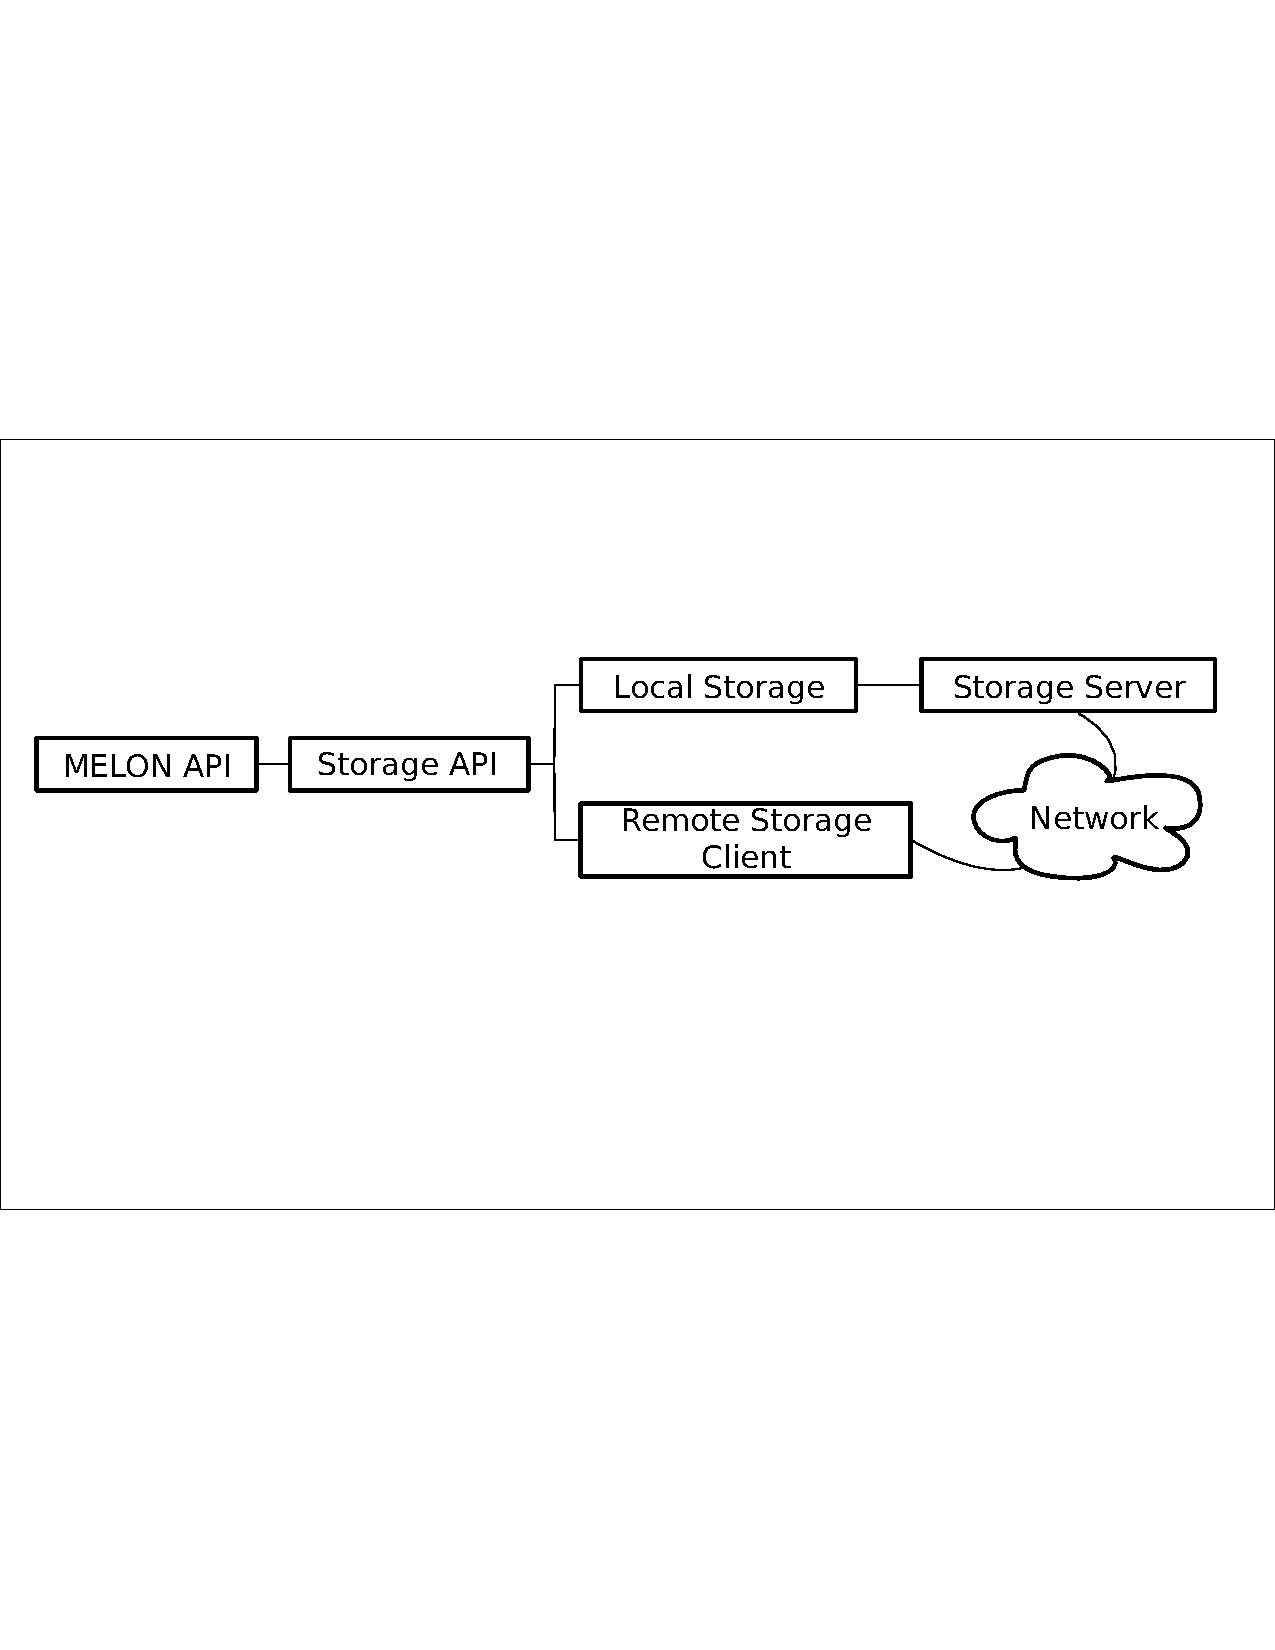
\includegraphics[scale = .70, clip, trim = 10px 280px 10px 250px]{figures/paradigm_arch.pdf}
\caption{Paradigm Architecture}
\label{fig:architecture}
\end{figure}

The architecture of our MELON implementation illustrated in Figure \ref{fig:architecture} is divided into five parts. The MELON API is the only interface exposed to the application and provides the six operations described above. The MELON API interacts with the distributed message storage through the storage API, which provides the same interface for both local and remote storage. The storage server proves a network interface to a local storage space and accepts connections made through the remote storage stub.

\section{MELON API}

The MELON API as provided to the application is very simple. It only provides the six MELON operations, plus the ability to manually specify remote hosts. The API implementation does very little except interact with either local or remote storage. Both local and remote storage offer the same API, so they can be accessed uniformly.

The prototype library tracks the local storage, remote servers, and read messages. \textbf{write} and \textbf{store} operate on the local storage only. \textbf{read} and \textbf{take} make no distinction between local and remote storage but simply iterate through the list of stores and invoke operations on them until the operation is satisfied. Each operation accesses the stores in a random order to spread the load and also provide a variety of sources.

\section{Storage API}

The storage API is an interface between the MELON API and either local or remote storage. In practice, however, the MELON API calls methods on the local storage directly. The API offers exactly the same six operations as MELON.

Remote storage is accessed through the remote storage client which implements the same API as local storage, except without \textbf{write}/\textbf{store} since those are only performed locally. Each remote host is represented with its own remote storage client. Internally, the remote storage clients manage connections with the remote storage servers.

\section{Local Message Store}\label{impl:localstore}

While applications view the message store as a single entity, it is actually the federation of local message stores hosted by each node running MELON. Each message in the network is by default stored on exactly one node, which is the node on which the application is running which performed the \textbf{store} or \textbf{write} operation. In other words, storing a message is a local operation. This allows MELON to provide atomicity for message removal with \textbf{take} and to ensure per-host FIFO ordering when returning matched messages.

Local storage is implemented simply as two dynamic arrays, one for \textbf{write}/\textbf{read} messages and the other for \textbf{store}/\textbf{take} messages. For atomic updates, the \textbf{write}/\textbf{read} array uses a readers/writer lock to allow multiple \textbf{read} operations to access the array in parallel, but locks the array for \textbf{write} operations. The \textbf{store}/\textbf{take} array does not permit concurrent operations, since both \textbf{store} and \textbf{take} modify the store. The two arrays may be accessed and modified independently.

Implementation of \textbf{store}/\textbf{write} is simple: exclusive access is obtained for the appropriate array and the message is appended  to the end. 

For \textbf{take}, the lock is obtained for the \textbf{store}/\textbf{take} array and the message store starts at the oldest message and linearly scans until a matching message is found. When a matching message is found, the message is removed from the array and the elements shift appropriately to fill the gap.

When performing a \textbf{read}, a readers lock for the \textbf{write}/\textbf{read} array is obtained. The message store starts at the oldest message and linearly searches the array for a matching message. If a message is matched, it must also be checked to not exist in the provided read message set (see Section \ref{sec:readmessages} below). If it is in the read message set, the search continues. Otherwise, the matching unread message is returned.

In the architecture described here, the local message store is unaware of the location of the requesting or storing client, although it is assumed \textbf{store}/\textbf{write} operations are local. The storage server provides an API for remote applications to connect to and query the local storage.

\section{Storage Server}

Each local storage is accompanied by a storage server which allows remote hosts to connect and query the local storage. The storage server handles incoming connections, converts queries into calls to the local storage, and converts messages from local storage into responses back to the remote hosts. Each storage server can handle multiple concurrent requests.

\section{Networking}

Network communication is handled using ZeroMQ\cite{hintjens2013zeromq}, a high performance, high level networking library. For the prototype, the network communication was intentionally kept simple. For example, a \textbf{read} request queries remote hosts in a random order and stops when a matching result is returned. For bulk operations, the prototype implementation also queries remote hosts in random order, but continues fetching results until all hosts have either returned a response or a timeout is reached.

While it is possible to improve upon this approach using multicast, it would greatly complicate the implementation by requiring the client to handle multiple asynchronous responses, choose between them, request the actual matching message, and then handle failure scenarios if the matching message cannot be returned. Our approach was to trade off potential performance gains for simplicity.

\section{Read Message Tracking}\label{sec:readmessages}

When a messages is stored, it is given a unique identifier [\textit{P}, \textit{M}], where \textit{P} is a globally unique integer identifier for the storing process, and \textit{M} is an integer identifier for the stored message. Each process maintains an integer ID which is incremented for each store. Messages stored from the same process with sequential \textbf{store} or \textbf{write} operations will have consecutive \textit{M} values and share the same \textit{P} value.

In order to prevent \textbf{read} from returning a message more than once in the same process, each process maintains a sparse bit set for each process from which a message has been read. The identifier [\textit{P}, \textit{M}] is condensed into a single unique integer \textit{Q} using the ``elegant pairing function''\cite{szudzikelegant} shown in Equation \ref{eq:elegantpairing}. Since the values of \textit{Q} will be consecutive integers for all consecutive values of $M < P$, it is helpful to set \textit{P} to be higher than the number of expected messages. The value \textit{Q} is then stored in a sparse bit set with a hash table using integer keys and bit field values.

 \begin{equation}
   f(M,P) = \left\{
     \begin{array}{lr}
       M^{2} + M + P & : M \geq P \\
       P^{2} + M & : M < P
     \end{array}
   \right.
   \label{eq:elegantpairing}
\end{equation}

The index \textit{i} in the sparse bit set indicates the range stored in the bit set. If \textit{w} is the number of bits for each bit set, then each bit field can store up to \textit{w} values of \textit{n}, where $w \times i \leq n < w \times (i + 1)$. A message with ID \textit{n} will be stored in index $n/w$ by setting the bit at $n \bmod w$ in the bit field to \texttt{1}.

If the index value is of size \textit{l} bits and the bit field contains \textit{w} bits, then the cost for storing a single value is $l + w$. For storing a set of consecutive values of length \textit{m}, the cost is $\lfloor \frac{m \times l}{w} \rfloor + m$ bits. In other words, the total cost is one bit per message, plus the cost of one index per \textit{w} messages.

\begin{table}
\centering
\caption{Sparse bit set example}
\begin{tabular}{|c|c|} \hline
Index & Bit Field \\ \hline
0 & 01100001 \\ \hline
4 & 00010000 \\ \hline
15 & 10100100 \\ \hline
\end{tabular}
\label{fig:bitset}
\end{table}

Consecutive messages (from any starting value) are the best-case scenario for sparse bit sets. In the worst case, the message IDs differ by at least \textit{w}, causing each message to incur a $l + w$ cost for storage and a total cost of $m \times (l + w)$ bits.

Determining if a message [\textit{P}, \textit{M}] is in the set is accomplished by first computing \textit{Q}. If there is no key at index $Q/w$, the message has not been read. Otherwise, retrieve the bit field \textit{b} at index $M / w$. If $b \wedge 2^{M \bmod w} \neq 0$ then the message has been read, otherwise the message is unread.

\subsection{Sparse Bit Set Performance}

For matching read-only messages, the read message data structure will need to be fast and small. In this section we are using a sparse bit set implementation developed for MELON\footnote{Source available at https://github.com/presidentbeef/dumb-numb-set} based on Ruby hashes and using 64-bit integers. Testing is performed using Ruby 2.1.2.

\begin{figure}
\centering
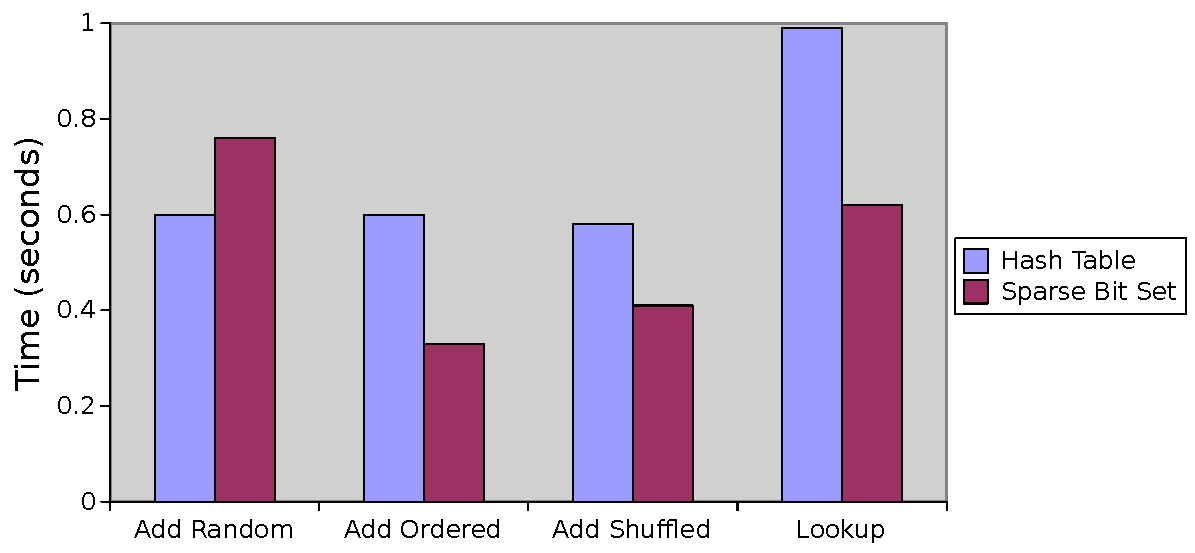
\includegraphics[width = \textwidth, scale = 0.75]{figures/bitset-speed.pdf}
\caption{Sparse Bit Set Operation Speed}
\label{fig:bitsetspeed}
\end{figure}

In Figure \ref{fig:bitsetspeed} we compare the speed of the sparse bit set implementation to the standard Ruby hash table implementation. The times reported for each operation are per 1 million records. The sparse bit set outperforms the hash table for each experiment except adding random numbers to the set. For the sparse bit set, adding an integer involves creating and storing two values: the index and the bit field. For the random values, this occurs more frequently. For sequential integers, the cost of creating the index and bit field is amortized over several stores (essentially the number of bits in the bit field).

\begin{figure}
\centering
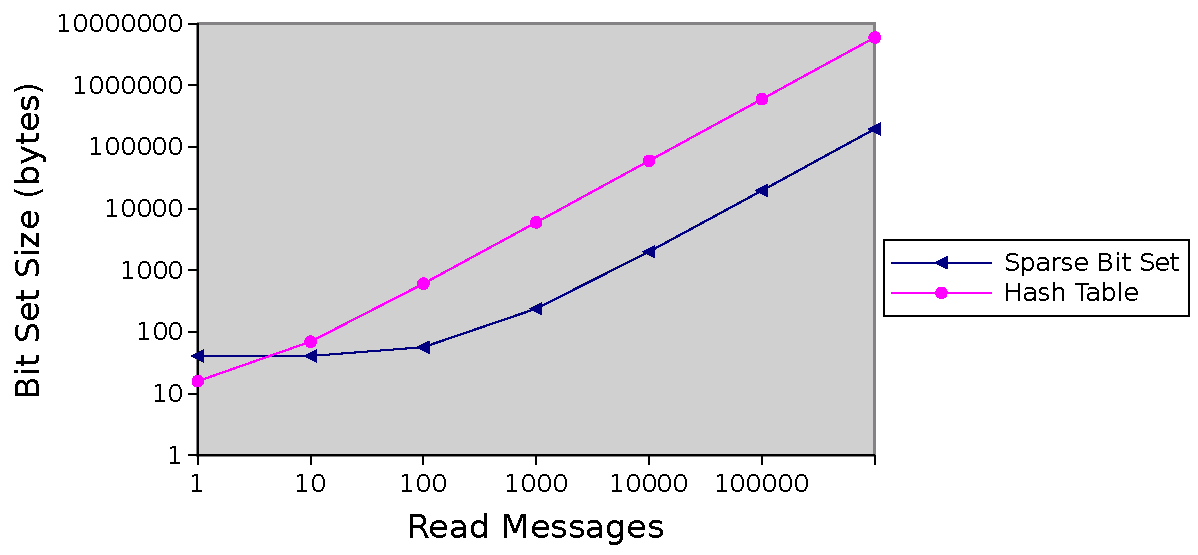
\includegraphics[width = \textwidth, scale = 0.80]{figures/bitset-size.pdf}
\caption{Sparse Bit Set Size}
\label{fig:bitsetsize}
\end{figure}

Figure \ref{fig:bitsetsize} shows the increase in the size of the bit set as the number of read messages increases. This is the actual serialized size of the data structure as it is sent over the network. After about 1,000 messages, the size grows linearly and averages 1.6 bits per message. At 1 million records, the data structure is about 192 KB. However, this is about 96\% smaller than the standard Ruby hash table.

Without pruning, the read message data structure will grow unbounded. There are some potential solutions to this. One solution would be to track read messages per host. When requesting a read-only message from a given host, only the read messages from that host are sent. Unfortunately, this ties applications to hosts and assumes messages will only be on the host which output them. This would prevent message replication as discussed in Section \ref{sec:replication}.

Since read messages may be garbage collected, hosts may provide feedback about which messages have been garbage collected. These messages may then also be garbage collected from the read data structure, essentially pruning it. This could be returned as optional data when a request for read-only messages is made, thereby avoiding any extra communication.

\section{Message Replication}\label{sec:replication}

Distributing copies of messages to multiple hosts can increase message availability when a host is temporarily unavailable, under heavy load, or even in the face of network partitioning. Additionally, it can improve performance if messages can be fetched from a nearer host or from multiple hosts in parallel. While not a requirement of the MELON paradigm, message replication may be implemented as an additional feature of MELON without adding any new operations although it does add complexity.

Take-only messages are generally not eligible for replication since their removal must be atomic. Coordinating removals for all replicated copies is not only impractical, it is impossible if a node containing a replicated message leaves the network. Read-only messages, however, are expected to be read many times and cannot be explicitly removed, making them a candidate for replication.

FIFO order (per host) must be maintained no matter which host may actually return the messages. When each host manages its own stored messages, ordering is easily accomplished. When messages are distributed and multiple copies of the same message are available from different hosts the problem is more challenging. However, each host is still aware of the order in which the messages should be returned.

Instead of sending a request for matching messages, a process requests a list of message IDs which would have fulfilled the request, in order. Each host responds with a list of matching message IDs, but only for messages output by that host. The requesting process can then request messages by ID rather than message templates. Any host may return the actual messages, either the original message or replicas. Since the requesting process will be aware of the correct ordering, it can ensure the FIFO ordering is maintained when returning messages to the application.

This approach still requires the original host to be available when the first request is sent, and it is limited to fetching messages which have already been output at the time of the request. As such, it is best fitted to bulk retrieval (\textbf{bulk\_read}) of messages.

One other type of message may be replicated. Take-only messages which are addressed to a specific receiver may also be safely replicated since they may only be removed by that receiver. The receiver can track which directed messages it has already taken and simply discard duplicates. Replicating messages which will only be needed once seems wasteful, though, except in the case where delivery of private messages is critical.

In any scenario, replicated messages would need to be kept in a separate storage from regularly output messages. Replicated messages would only be returned to requests by message ID or for directed take-only messages. A background process would be needed to replicate the messages out to different hosts. A mechanism would also be needed to determine when to replicate the messages, and when to garbage collect replicas. Overall, message replication requires a considerable amount of added complexity and overhead to MELON.

\section{Garbage Collection}

The MELON model explicitly acknowledges memory and storage are especially limited on mobile devices. For simplicity, in this section we consider this to be an absolute limit on the number of messages to be stored at any time. This is inexact in relation to the actually memory used since messages may vary in size.

Since MELON persists messages and read-only messages cannot be removed by applications, it would not be difficult for an application to exhaust available space on a device. This is an issue for any paradigm which persists its messages but most proposals do not address it. When there is no more space to store a message, a communication paradigm implementation may crash, raise an exception, simply drop the message, or perform garbage collection to remove existing messages and free space for new ones.

To offset its otherwise permanent storage of read-only messages, MELON implementations should have a mechanism to remove old messages. MELON's requirements for garbage collection straddle memory management garbage collection and cache eviction. In memory management, any references to a value in memory will require it to be kept, but MELON messages do not have direct references and we cannot know which messages may be needed in the future. This is similar to maintaining a cache, in which the same limitation of knowledge applies. Unlike a cache, there are generally no other copies of the message available to fall back upon. Once evicted from the MELON store, the message is lost.

First-in first-out (FIFO) and least-recently used (LRU) are basic strategies for choosing which messages to replace in storage. For MANET applications, there is often a few messages which are expected to be available for extended periods of time - for example, messages containing identity of nodes or other static data. This suggests simply discarding the oldest messages might not be the best approach. When evicting by LRU, it is necessary to track the last access time for each message. When deciding which messages to remove, the LRU policy drops the messages with the oldest access time. This is probably a good fit for MELON, but there are also more sophisticated variants on LRU which may be useful. Determining what replacement strategy is best for MELON is a topic for future work.

Besides determining which messages should be removed from storage, it is also necessary to have a policy for when to perform garbage collection. Unlike memory garbage collection, MELON garbage collection is not expected to have a significant impact on performance. MELON garbage collection does require locking the store to actually remove the messages, but the determination of which messages to remove may be performed without locking since it does not need to be exact. One approach is to only perform garbage collection when the message limit is actually reached, then to remove either a single message or a percentage of messages. Removing more messages reduces frequency of garbage collection, but increases the time spent removing messages each time.

Since MELON messages need to be stored in FIFO order, garbage collection does require some form of compacting to ensure new messages may be added at the end of the queue.

Fitting the best garbage collection strategy to MELON remains as future work.

\chapter{Case Studies}

\section{News Server/Reader}

\section{Chat Application}

\section{Experiment Coordinator}

\begin{figure}
\centering
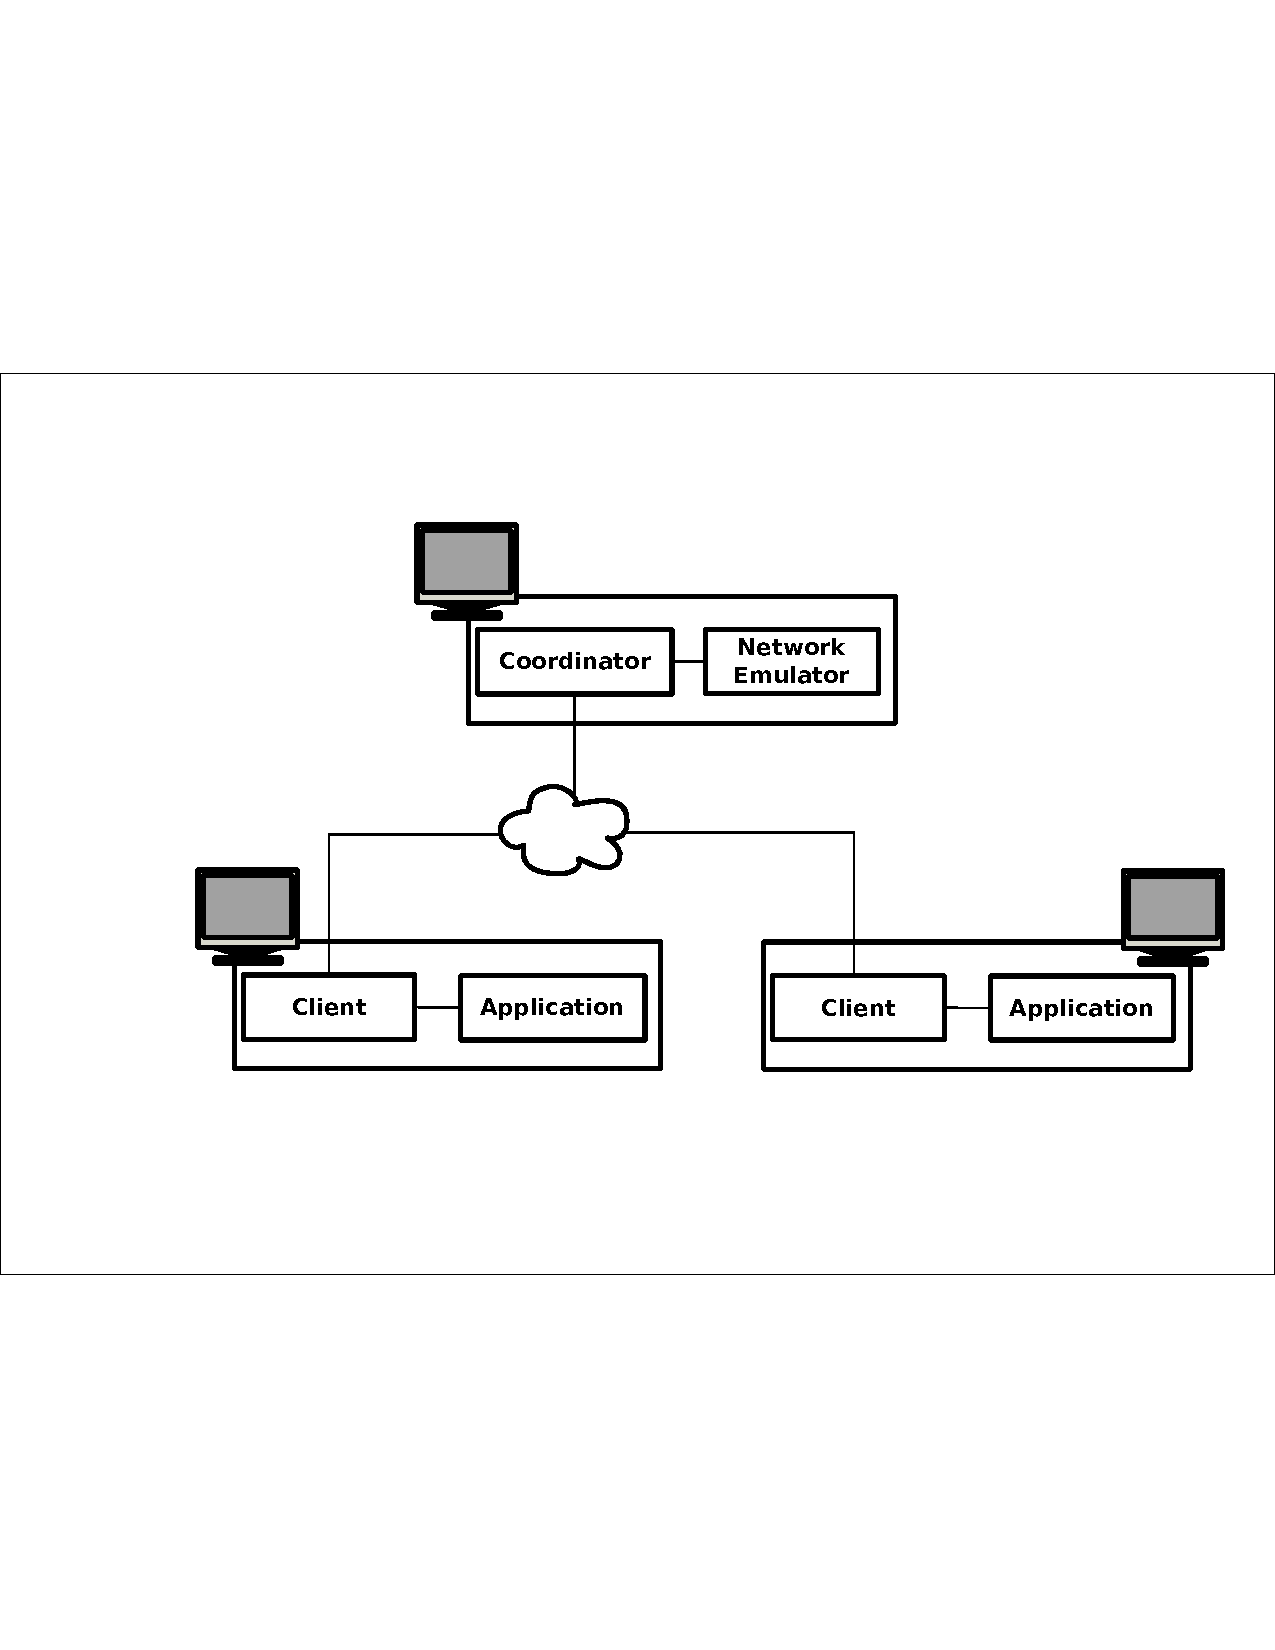
\includegraphics[scale = .34, clip, trim = 94px 279px 24px 252px]{figures/experiment_arch.pdf}
\caption{Coordinator Architecture}
\label{fig:coordarchitecture}
\end{figure}

To ease the process of repeatedly setting up experiments, we developed an experiment coordination framework written with MELON. The application handles running real applications on multiple hosts, executing the network emulator, and gathering results into a single location.

The architecture of the framework is illustrated in Figure \ref{fig:coordarchitecture}. For simplicity, the coordinator resides on the same host as the network emulator. The coordinator sends out commands to clients which reside on each host. The clients are responsible for executing programs on their local host and sending resulting output to the central coordinator.

The coordinator first writes a job containing the command to execute and any relevant options. Each client reads the job, starts the command, then stores a confirmation once the application is initialized and ready to begin. When the coordinator has taken a confirmation from each host, it starts the network emulator, then writes a ``go'' message. Upon reading the go message, each client signals the application to begin.

As the application runs, the client gathers output and stores it. When the application finishes, it signals that it is done and then awaits a kill signal from the client. The client also stores a ``done'' signal. When the coordinator has taken a ``done'' message from each client, it collects the results and then sends a ``stop'' message. The clients then stop the applications and the framework is ready to start the next experiment.

\section{Shared Whiteboard}

\section{Shared Whiteboard Example}\label{sec:wb}

A shared whiteboard is a digital document which may be edited and viewed by multiple users concurrently and is commonly proposed as an example of an application well-suited to MANETs\cite{wb5}\cite{wb6}. Shared whiteboards are distributed, real-time, and interactive, which presents some interesting characteristics. Since many participants may be updating the whiteboard, ordering of changes is very important to maintain a consistent document. It is also important that changes be propagated quickly so that each user is working with the latest document.

We have implemented a shared whiteboard in MELON, publish/subscribe, RPC, and tuple spaces using JRuby (a Java implementation of the Ruby language) in order to compare their features and performance.
Each version shares common code related to the actual whiteboard itself, which is implemented in the \texttt{Whiteboard} class.
Changes to the shared whiteboard are encapsulated in a \texttt{Figure} object. Each version implements an \texttt{add\_local\_figure} method which is called when the user modifies the shared whiteboard.
The MELON and tuple space versions also implement an \texttt{add\_remote\_figures} method which is used to retrieve updates from remote nodes.

\subsection{Publish/Subscribe}

The publish/subscribe paradigm divides processes into publishers and subscribers. In topic-based publish/subscribe, publishers simply publish messages tagged with a topic identifier. Subscribers receive the messages by subscribing to one or more topics and specifying a callback to handle the publications asynchronously and separately from the main process thread. It is also possible to handle multiple incoming publications concurrently. Publish/subscribe does not guarantee any ordering of publications nor does it specify how to deliver messages if the subscribers is not available at the time of publication. In distributed publish/subscribe such as MANETs, it is generally not expected that publishers would persist and deliver messages at a later time\cite{psfaces}.

The publish/subscribe whiteboard in Table \ref{fig:pswb} sets up a subscription to the ``whiteboard" topic and a callback to add remotely published figures to the whiteboard. This allows the whiteboard to receive updates at any time in a separate thread, which is precisely what would be desired. To output a new figure, the whiteboard simply publishes the figure to the ``whiteboard" topic.

\begin{table}
\centering
\begin{tabular}{c c}
\begin{minipage}{2.75in}
\begin{verbatim}
require "ps"
require "whiteboard"

class PSWhiteboard < Whiteboard
  def initialize
    @ps = PS.new
    
    @ps.subscribe("whiteboard") do |figure|
      add_figure(figure)
    end
  end

  def add_local_figure(figure)
    @ps.publish("whiteboard", figure)
  end
end
\end{verbatim}
\caption{Publish/Subscribe Whiteboard}\label{fig:pswb}
\end{minipage}
&
\begin{minipage}{2.5in}
\begin{verbatim}
require "rpc"
require "whiteboard"

class RPCWhiteboard < Whiteboard
  def initialize
    @rpc = RPC.new
    @rpc.export(self)
  end

  def add_local_figure(figure)
    wbs = @rpc.find_all("RPCWhiteboard")
    wbs.add_figure(figure)
  end
end


\end{verbatim}
\caption{RPC Whiteboard}\label{fig:rpcwb}
\end{minipage}
\end{tabular}
\end{table}


\subsection{RPC}

Remote procedure calls (RPC) is a distributed programming paradigm which disguises remote communication as local method calls. A host can ``export" an object to be accessed remotely. Remote hosts discover these remote objects by name and then invoke methods on them. Arguments may be passed to the remote method and the return value of the method is returned to the local process. A variation of this used in our example is group RPC, which allows us to invoke the same method with the same arguments on all known remote objects of the requested type. These calls are performed asynchronously. Typically the return values would be handled by a callback, but this functionality is not used in our example.

A shared whiteboard implementation using RPC is listed in Table 5. When the whiteboard is initialized, it exports itself as a remote object. This allows other hosts to remotely invoke the \texttt{add\_figure}. Like publish/subscribe, this allows the whiteboard to accept remote figures asynchronously from the main process thread and is a natural feature of RPC. Distribution of remote figures is performed by first finding all remote instances of \texttt{RPCWhiteboard}, then invoking the \texttt{add\_figure} method (defined on the parent class) directly, passing in the new figure as an argument. Since the group RPC is asynchronous, it is possible that a call might complete before a prior call.

\subsection{Tuple Spaces}

Tuple spaces operate on a distributed shared memory space of ordered tuples. Tuples may be output using the \textbf{out} operation, then retrieved using \textbf{rd}, which copies the tuple, or \textbf{in}, which removes the tuple from the tuple space based on matching templates. If multiple tuples match a template, one of the matching tuples is chosen nondeterministically to be returned.

Table \ref{fig:tswb} shows the tuple space version, which is very similar to MELON. To send an update, it outputs a tuple containing just the new figure. Unlike MELON, a misbehaving or misconfigured client could remove the messages from the tuple space, disrupting the shared whiteboard communication. Retrieval of remote messages uses a \textbf{bulk\_rd} operation to read all messages containing a figure. To continuously retrieve messages asynchronously, this method can be called inside a loop in a separate thread. Once a group of figures is retrieved, each individual figure is added to the local whiteboard.

Tuple spaces suffer from the multiple read problem\cite{mrdp}: repeated nondestructive read operations (\textbf{rd}) may return any matching tuple, including the same tuple. As discussed in \cite{mrdp}, one solution is to use a mutex tuple to gain exclusive access to the tuple space, remove all the desired tuples using \textbf{in}, then replace all the tuples and release the mutex. However, this approach prevents concurrent access and is dangerous in a MANET where the node holding the mutex may disappear. Another solution is to use a counter in each tuple, then read tuple 0, then tuple 1, and so on. Then each process can request tuples by the counter value. However, if multiple processes are producing tuples they must coordinate to produce consistent counters, essentially resulting in a producer-side mutex.

Finally, \cite{mrdp} proposes a \textbf{copy-collect} operation, which copies all matching tuples. We have implemented this as the \textbf{bulk\_rd} operation as used in Table \ref{fig:tswb}. However, this does not solve what might be termed the ``multiple multiple read problem": since our tuple space is not static, reading all matching tuples once is not sufficient. We need to be able to perform multiple \textbf{bulk\_rd}s to get all figures added to the whiteboard. Without \textit{a prior} knowledge of remote hosts in the system, the only option which allows concurrent access to the tuple space is to read \textit{all} matching tuples. Naturally, this becomes quite expensive as the number of tuples grows.

\begin{table}
\centering
\begin{tabular}{c c}
\begin{minipage}{2.75in}
\begin{verbatim}
require "melon"
require "whiteboard"

class MelonWhiteboard < Whiteboard
  def initialize
    @melon = Melon.new
  end
  
  def add_local_figure(figure)
    @melon.write([Figure])
  end

  def add_remote_figures
    figures = @melon.read_all([Figure])

    figures.each do |figure|
      add_figure(figure[0])
    end
  end
end
\end{verbatim}
\caption{MELON Whiteboard}\label{fig:mwb}
\end{minipage}
&
\begin{minipage}{2.5in}
\begin{verbatim}
require "tuplespace"
require "whiteboard"

class TSWhiteboard < Whiteboard
  def initialize
    @ts = Tuplespace.new
  end

  def add_local_figure(figure)
    @ts.out([Figure])
  end

  def add_remote_figures
    figures = @ts.bulk_rd([Figure])

    figures.each do |figure|
      add_figure(figure[0])
    end
  end
end 
\end{verbatim}
\caption{Tuple Space Whiteboard}\label{fig:tswb}
\end{minipage}
\end{tabular}
\end{table}

\subsection{MELON}

The MELON whiteboard in Table \ref{fig:mwb} writes out each figure in a tuple containing just the new figure. It uses the \textbf{write} operation since every remote node needs to be able to read the figures. To retrieve remote figures, MELON uses \textbf{read\_all} to nondestructively read all messages containing a \texttt{Figure}. Like tuple spaces, the \texttt{add\_remote\_figures} method should be called in a separate thread to provide asynchronous updates. Unlike tuple spaces, MELON's \textbf{read\_all} operation only retrieves unread messages, eliminating the ``multiple multiple read" problem.

MELON directly provides three features which are helpful to the whiteboard application: persistent messages, reading only unread messages, and returning messages in a per-host ordering. Message persistence is crucial in MANET applications, where communication with remote nodes is often disrupted and delayed. For a shared whiteboard, every message must be delivered to keep the document synchronized between users. By managing read versus unread messages, MELON easily allows the whiteboard to efficiently fetch only newly-added figures. Finally, MELON guarantees the updates from each host will be retrieved in the order that host initiated them. While this does not provide a global ordering, it does ensure updates from a single host will be in order.


\chapter{Evaluation}

\section{Performance Analysis}

\subsection{Operation Speed}

\begin{figure}
\centering
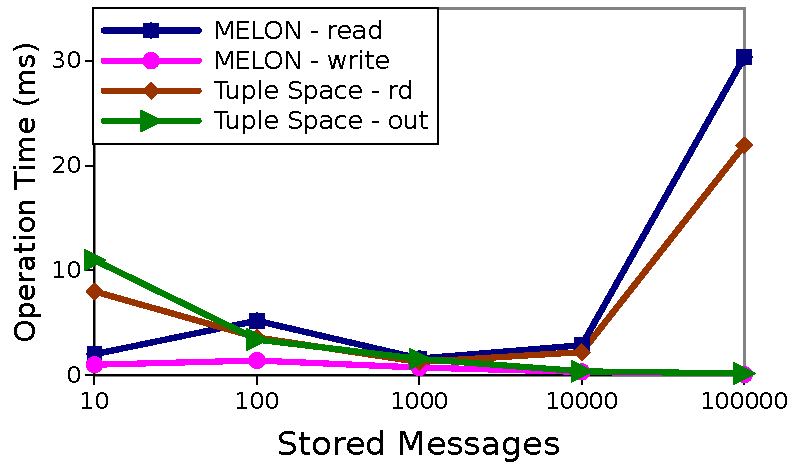
\includegraphics[width = \linewidth, clip, trim = 0px 0px 0px 0px]{figures/read_speed.pdf}
\caption{Read Speed}
\label{fig:readspeed}
\end{figure}

\begin{figure}
\centering
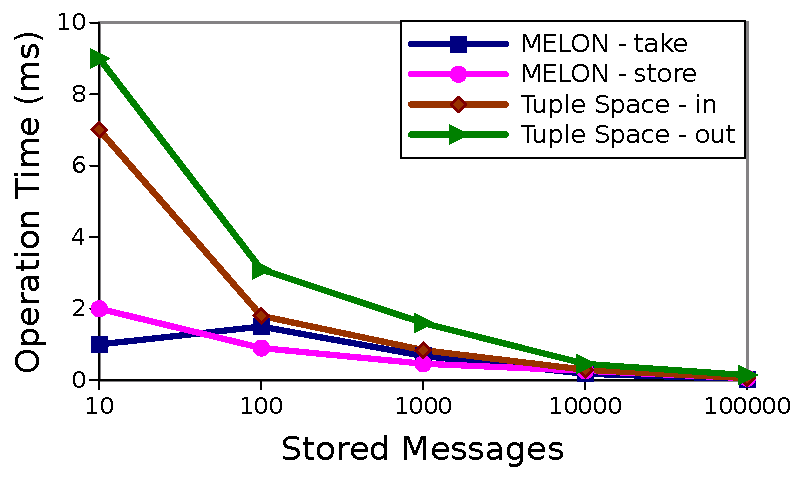
\includegraphics[width = \linewidth, clip, trim = 0px 0px 0px 0px]{figures/in_speed.pdf}
\caption{Take Speed}
\label{fig:takespeed}
\end{figure}

To establish a baseline for performance, we measured the time for the \textbf{write}, \textbf{read}, \textbf{store}, and \textbf{take} operations directly on a local message storage and compared the results to the LighTS\cite{lights} local tuple space implementation used by LIME. In these experiments, all messages are first stored, then either read or removed from the local storage. No network communication is involved.

When comparing \textbf{read} and \textbf{rd}, we simulate the MELON's feature of only returning unread messages by using a sequential integer ID in the tuples and performing a \textbf{rd} operation for each ID. If we did not do this, LighTS would return the same tuple for each \textbf{rd} operation.

In both LighTS and MELON, messages are stored in what is essentially an array. Since we are not removing messages, each operation must linearly search the array taking O(\textit{nm}) time, where \textit{n} is the length of the message or tuple and \textit{m} is the number of stored messages or tuples. Naturally, operations returning messages near the beginning of the array are faster, while the slowest operation returns the last message in the array. In our experiments, this cost did not become apparent until searching 100,000 messages. The average time per operation from 10,000 to 100,000 increased \~9x for LighTS and \~10x for MELON, with total read time taking just under a minute. It is unsurprising MELON is slightly slower, since it must also check that a message is not in the ``read'' list before returning it.

On the other hand, removing messages is naturally quite fast, since the matching message is always the first message in the store. All \textbf{take}/\textbf{in} operations require less than 8\textit{ms} to execute on average. MELON is slightly faster here due to differences in how removal is implemented, although average speed per operation converges as the number of operations performed increases.

Storing messages is faster than removing them for both implementations. In LighTS there is slightly more constant overhead for adding new tuples, so \textbf{out} operations are a little slower than \textbf{write} and \textbf{store} in MELON.  However, in reality both implementations are plenty fast for typical applications, since storing a message takes less than 10\textit{ms} on average, and usually less than 4\textit{ms}.

Overall, MELON performs roughly the same or better than LighTS when performing serial operations.

\subsection{Communication Overhead}

\begin{figure}
\centering
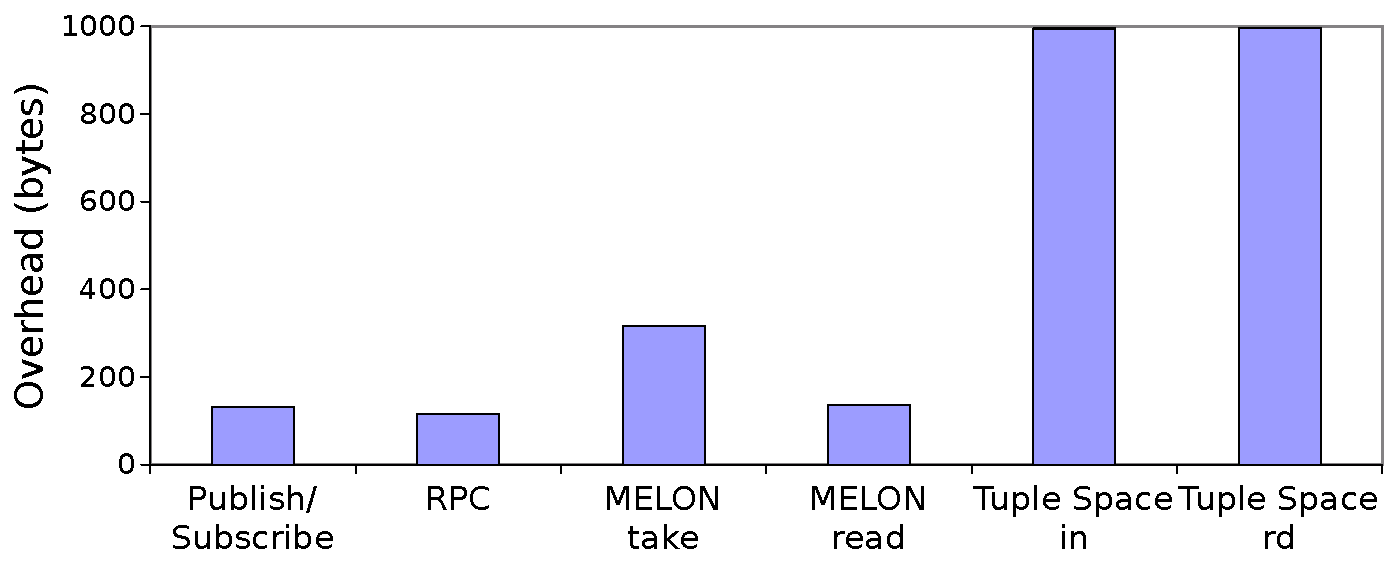
\includegraphics[scale = .50, clip, trim = 0px 0px 0px 0px]{figures/overhead.pdf}
\caption{Message Overhead}
\label{fig:overhead}
\end{figure}

For any communication library or framework, the message size added by use of the library is an important factor in determining its usefulness. In these experiments, we measure the number of bytes actually sent over the network, divide by the number of messages sent (in this case, 1000) and subtract the 1KB application payload. This leaves us with the overhead introduced by the paradigm. We compare the overhead of MELON to canonical implementations of publish/subscribe, RPC, and tuple spaces in Figure \ref{fig:overhead}.

Publish/subscribe and RPC have very low overhead and provide a good baseline. In the case of publish/subscribe, the only added information to a publication is the topic. Periodic subscription messages are small and infrequent compared to the number of messages sent. For RPC, there is one initial exchange to find the remote object, then later messages only need the object and method names plus the payload itself.

As in the operation speed experiments, we use the LighTS tuple space implementation. The serialized versions of tuples and tuple templates are very large and must be sent for each request. If a simpler data structure were used, overhead would be expected to be similar to MELON's overhead for \textbf{take}.

For MELON, \textbf{take} and \textbf{read} requests must send a message template, so the size of the request is dependent on how many values the template contains. For \textbf{read} operations, each request must also send information on previously read messages as described in Section \ref{sec:readmessages}, which increases as the number of read messages increases.

\subsection{Message Latency}

\begin{figure}
\centering
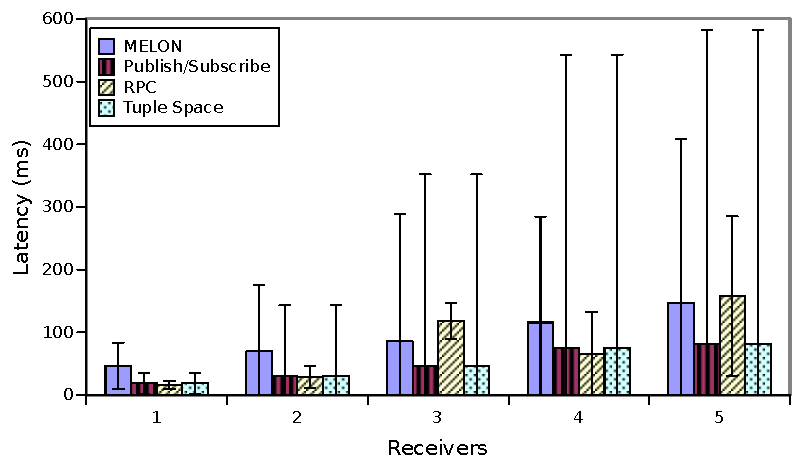
\includegraphics[width = \linewidth, clip, trim = 0px 0px 0px 0px]{figures/latency_static.pdf}
\caption{Message Latency - Static Scenario}
\label{fig:latencystatic}
\end{figure}

\begin{figure}
\centering
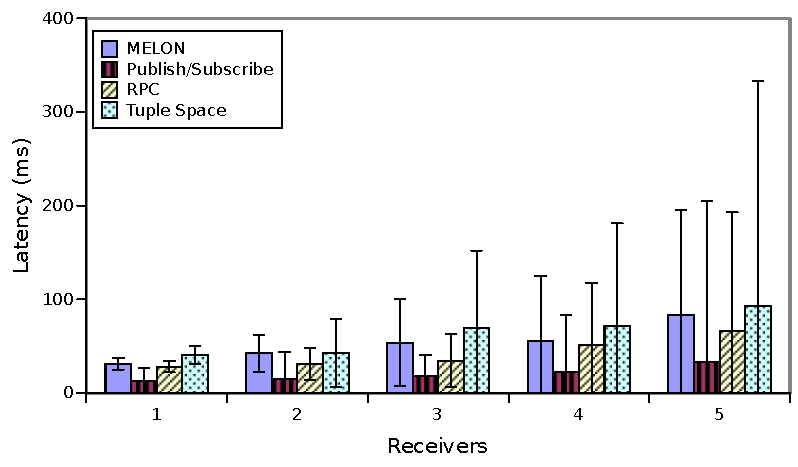
\includegraphics[width = \linewidth, clip, trim = 0px 0px 0px 0px]{figures/latency_mobile.pdf}
\caption{Message Latency - Mobile Scenario}
\label{fig:latencymobile}
\end{figure}

Figures \ref{fig:latencystatic} and \ref{fig:latencymobile} show the average latency between a client's request for a message and the receipt of a matching message. The error lines indicate the standard deviation. In these experiments, a single host writes out 1,000 messages with a 1KB payload, and the other hosts concurrently read the messages. Tuple spaces and MELON used the \textbf{rd}/\textbf{read} operations to retrieve the messages one at a time, rather than the bulk retrieval with \textbf{rdg} or \textbf{read\_all}. Since publish/subscribe does not involve a ``request'' beyond the initial operation, latency was measured as the time elapsed between receiving sequentially numbered publications.

MELON does show higher average latency rates in the static scenario, although for three or more receivers the standard deviation is lower than the other paradigms. In the more realistic mobile scenario, however, MELON latency is about the same or slightly lower than tuple spaces. Comparing the static and mobile scenarios also demonstrates one of the issues in wireless networks: the mobile scenario allows distinct routes to form between hosts with less interference, while the static scenario has many collisions causing more communication delays even though the distance between devices is smaller.

\subsection{Message Throughput}

\begin{figure}
\centering
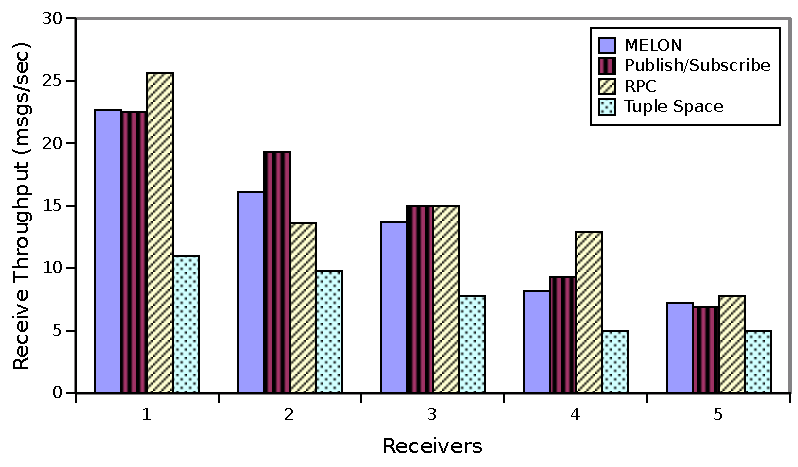
\includegraphics[width = \linewidth, clip, trim = 0px 0px 0px 0px]{figures/throughput_static.pdf}
\caption{Message Throughput - Static Scenario}
\label{fig:throughputstatic}
\end{figure}

\begin{figure}
\centering
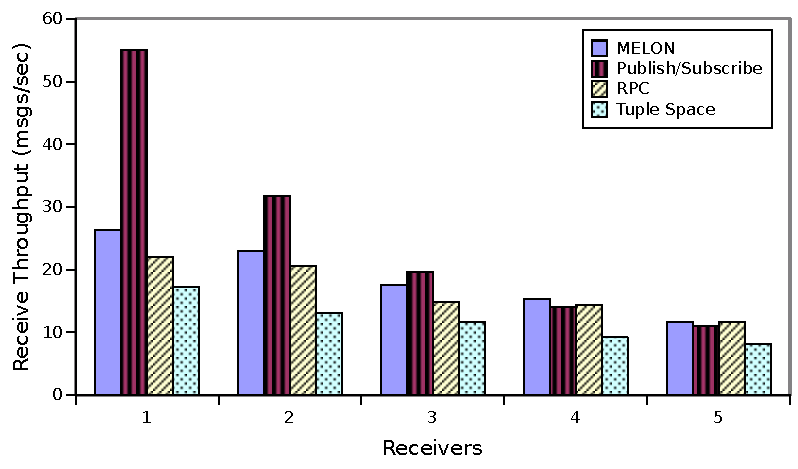
\includegraphics[width = \linewidth, clip, trim = 0px 0px 0px 0px]{figures/throughput_mobile.pdf}
\caption{Message Throughput - Mobile Scenario}
\label{fig:throughputmobile}
\end{figure}

Throughput in these experiments was measured on the receiver side in terms of messages delivered per second. As in the other experiments, 1,000 messages with a 1kb payload are output by one host, while the other hosts read the messages one at a time. Figures \ref{fig:throughputstatic} and \ref{fig:throughputmobile} show the average throughput as the number of receivers increases.

Publish/subscribe dominates in these experiments since it is the only push-based paradigm, allowing the sender to publish messages at a high rate without requests or acknowledgments from the receivers. Also, subscribers may receive multiple publications concurrently which increases throughput capacity.

Despite having higher average latency than the other paradigms, MELON demonstrates good throughput in both the static and mobile scenarios. However, throughput for all paradigms drops off dramatically as more receivers are added. Also, all paradigms performed better in the mobile scenario than in the static scenario. This is likely due to two factors: devices were not forced to be more than one hop apart, and the large number of devices allows distinct routes between devices and decreases wireless broadcast collisions.


\subsection{Whiteboard Performance}

For each implementation, we measured the number of messages lost, the number of messages received out of order, and the message latency. For out-of-order messages, we divided it into two metrics: host out-of-order and global out-of-order. Host out-of-order messages are messages from a single host which are not received in the order sent. Global out-of-order messages are those received before their preceding message. For example, if node A receives a message \textit{m}$_{1}$ from node B, then sends \textit{m}$_{2}$. If node C receives \textit{m}$_{2}$ prior to \textit{m}$_{1}$, \textit{m}$_{2}$ will be considered out of order.

\begin{figure}[ht]
\centering
\begin{minipage}[b]{0.48\linewidth}
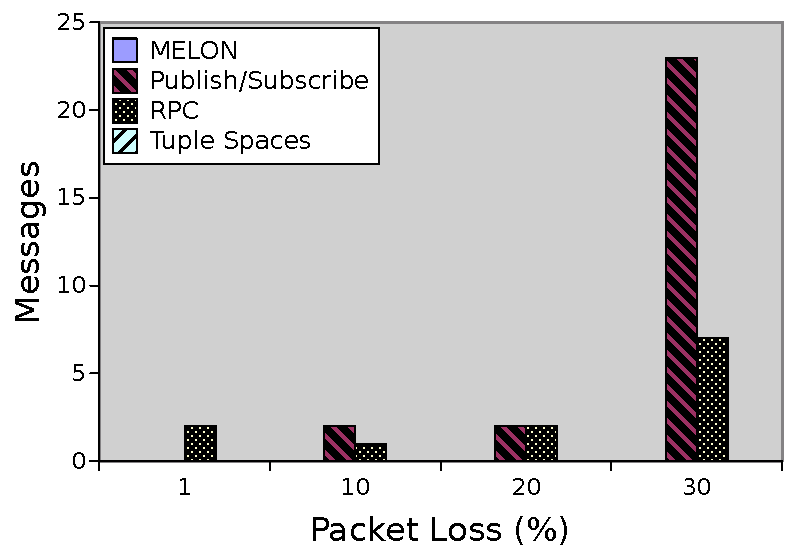
\includegraphics[width = \textwidth]{figures/hooo.pdf}
\caption{Host Out-of-Order Messages}
\label{fig:hooo}
\end{minipage}
\quad
\begin{minipage}[b]{0.48\linewidth}

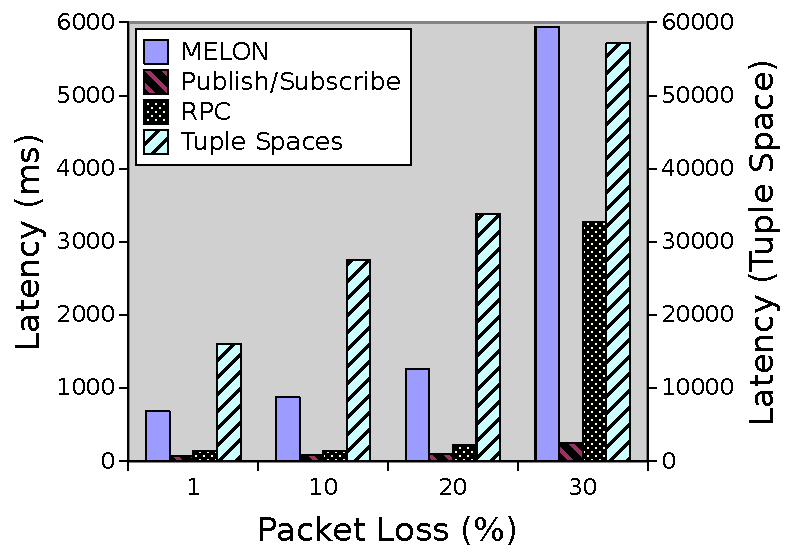
\includegraphics[width = \textwidth]{figures/latency.pdf}
\caption{Message Latency}
\label{fig:latency}
\end{minipage}
\end{figure}
\begin{figure}[ht]
\centering
\begin{minipage}[b]{0.48\linewidth}
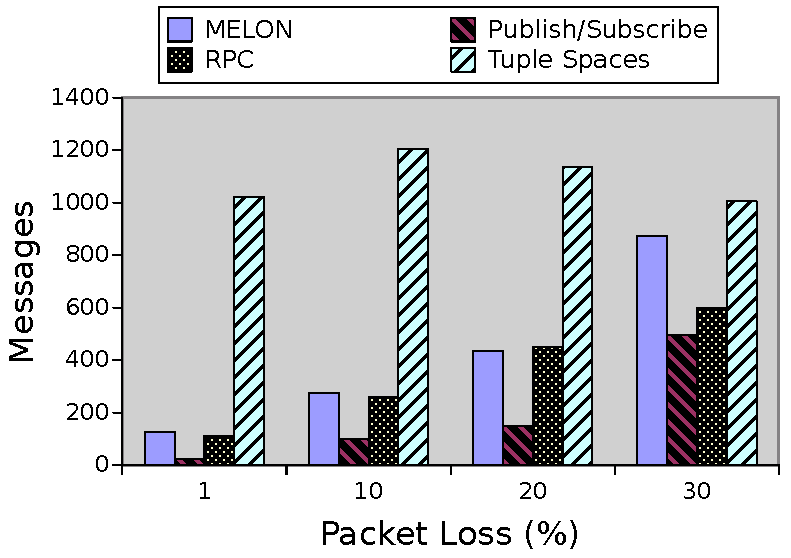
\includegraphics[width = \textwidth]{figures/gooo.pdf}
\caption{Global Out-of-Order Messages}
\label{fig:gooo}
\end{minipage}
\quad
\begin{minipage}[b]{0.48\linewidth}
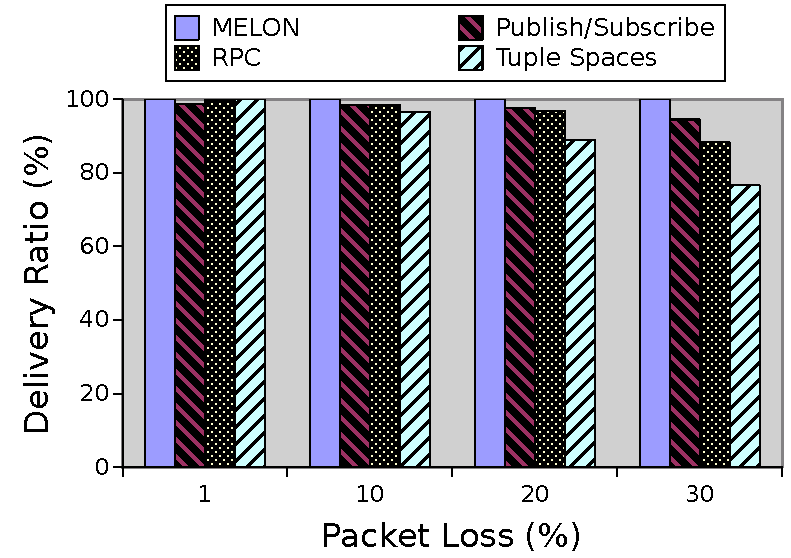
\includegraphics[width = \textwidth]{figures/delivery.pdf}
\caption{Delivery Rates}
\label{fig:delivery}
\end{minipage}
\end{figure}

In our experiments, messages from a single host were generally delivered in the order they were sent as shown in Figure \ref{fig:hooo}. For MELON and tuple spaces, no messages were delivered out of order. However, it should be noted that for tuple spaces this is an accident of the implementation, whereas in MELON it is guaranteed. In LighTS, tuples are sequentially stored locally in an array in the order they are output, then returned in that same order when they are matched. Tuple spaces in general do not return matched messages in any particular order.

In this application, RPC is used in an asynchronous manner since it is providing group communication. If one call is delayed, it is possible a subsequent call will complete before a prior one, which explains why RPC delivers a small number of messages out of order. Publish/subscribe is fully asynchronous and incoming publications can even be processed concurrently. However, even in the worst case publish/subscribe delivers 97.8\% of the messages from a host in the order they were sent. Unfortunately, like tuple spaces this is just the result of a single implementation and the RPC and publish/subscribe paradigms make no promises about the ordering of messages.

Unlike per-host ordering, many messages were delivered out of order from a global perspective as can be seen in Figure \ref{fig:gooo}. This is entirely expected, since none of the paradigms provide a global ordering. Enforcing a global ordering in an unreliable network is not feasible, since nodes may become unavailable at anytime while continuing to output messages. However, the global ordering remains important for a shared whiteboard.

Our results show publish/subscribe performs the best for this metric. Indeed, ordering is largely dependent on deliveries completing quickly before later messages overtake them. As shown in Figure \ref{fig:latency}, publish/subscribe is an extremely quick method for delivering messages, so it excels in ordering as well. Conversely, tuple spaces fare the worst, delivering 67\% of messages out of order. Again, because tuple spaces provide no way of controlling which matches messages are returned or in what order, the whiteboard implementation must transfer large amounts of tuples in order to nondestructively read all matching messages. This is extremely slow, as reflected in Figure \ref{fig:latency}.

MELON and RPC perform about the same for global ordering, although MELON is more affected when the network conditions worsen. This is likely due to MELON's reliable message delivery (Figure \ref{fig:delivery}), since some messages may be delayed significantly by broken network routes or network partitioning. In contrast, losing messages can improve ordering since a message not delivered cannot be out of order. Of the paradigms compared, MELON is the only one to demonstrate 100\% message delivery. Tuple spaces would also be expected to be reliable, but again in this application it is required to deliver large amounts of messages. Given that the median latency for tuple spaces reached a full minute, the experiment completed before some messages arrived.

While we have seen publish/subscribe have low delivery ratios in the past\cite{collins2010quantitative}, here it performs well in the lossy environment due to its quick delivery rates, but still dropped 1.4\% of messages when the network connectivity was good. RPC performs predictably, slowing losing more messages as the network degrades. Again, we are using group RPC, which means the application is not aware of how many receivers may be available and therefore does not retry to complete calls if a host cannot be reached for a period of time. Fully synchronous RPC would block the process until the message is delivered. However, that would also delay deliveries considerably which is not acceptable for a whiteboard application.

Median time between sending and receiving a message is reported in Figure \ref{fig:latency}. Since tuple spaces are so much slower, the results are aligned with the right-hand y-axis which is an order of magnitude higher. Publish/subscribe was extremely quick, which is expected since it requires no message confirmations nor active discovery of remote hosts. RPC was also quite fast until it was slowed down along with the other paradigms by the 30\% packet loss.

Logically, delivery rates and latency are directly related. With reliable delivery some messages may be very late, increasing overall latency. On the other hand, dropped messages do not count towards the latency metric, so a lossy communication paradigm can appear to be very fast. MELON errs on the side of reliability, and therefore is a bit slower as the network becomes less reliable and more delivery attempts are required. There is an additional trade-off that pull-based paradigms like MELON and tuple spaces must make, which is the frequency of the pull attempts. Publish/subscribe and RPC may send as soon as a message is ready, but MELON and tuple spaces must continually poll to receive messages. Faster polling results in faster message delivery, but higher overall network usage, collisions and resource monopolization.


\chapter{Conclusions}\label{chapter:conclusions}

\section{Results}

\section{Future Work}


\bibliography {refs}    % bibliography references
\bibliographystyle {uclathes} % or uclathes??

\end {document}

